% -------------- CR postFit 2J ---------
\begin{figure}[h]
  \centering
    \subfigure[]{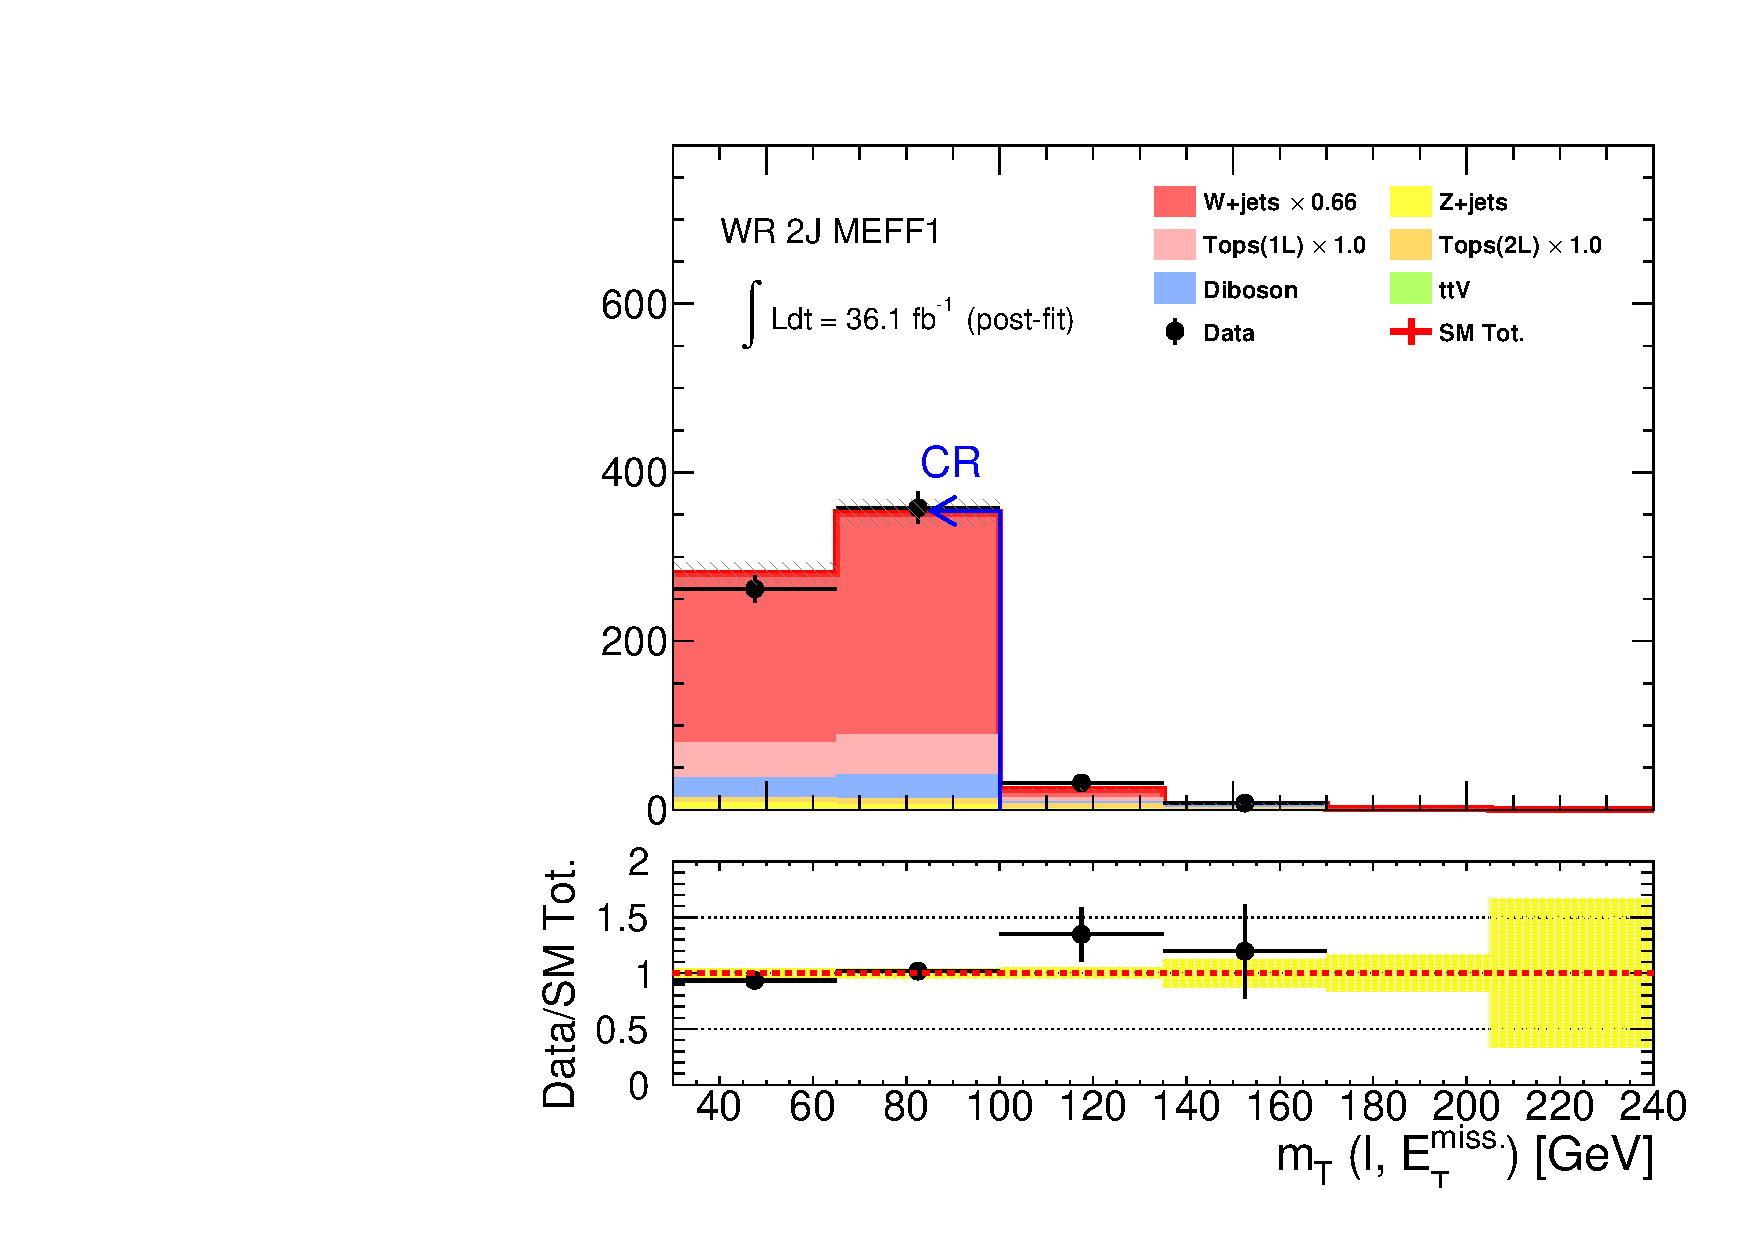
\includegraphics[width=0.41\textwidth]{figures/BGestimation/CRpostFit/WR2JMEFF1/mt__WR2JMEFF1_no_mt_postFit_2SFconfig_noYields.pdf}}
    \subfigure[]{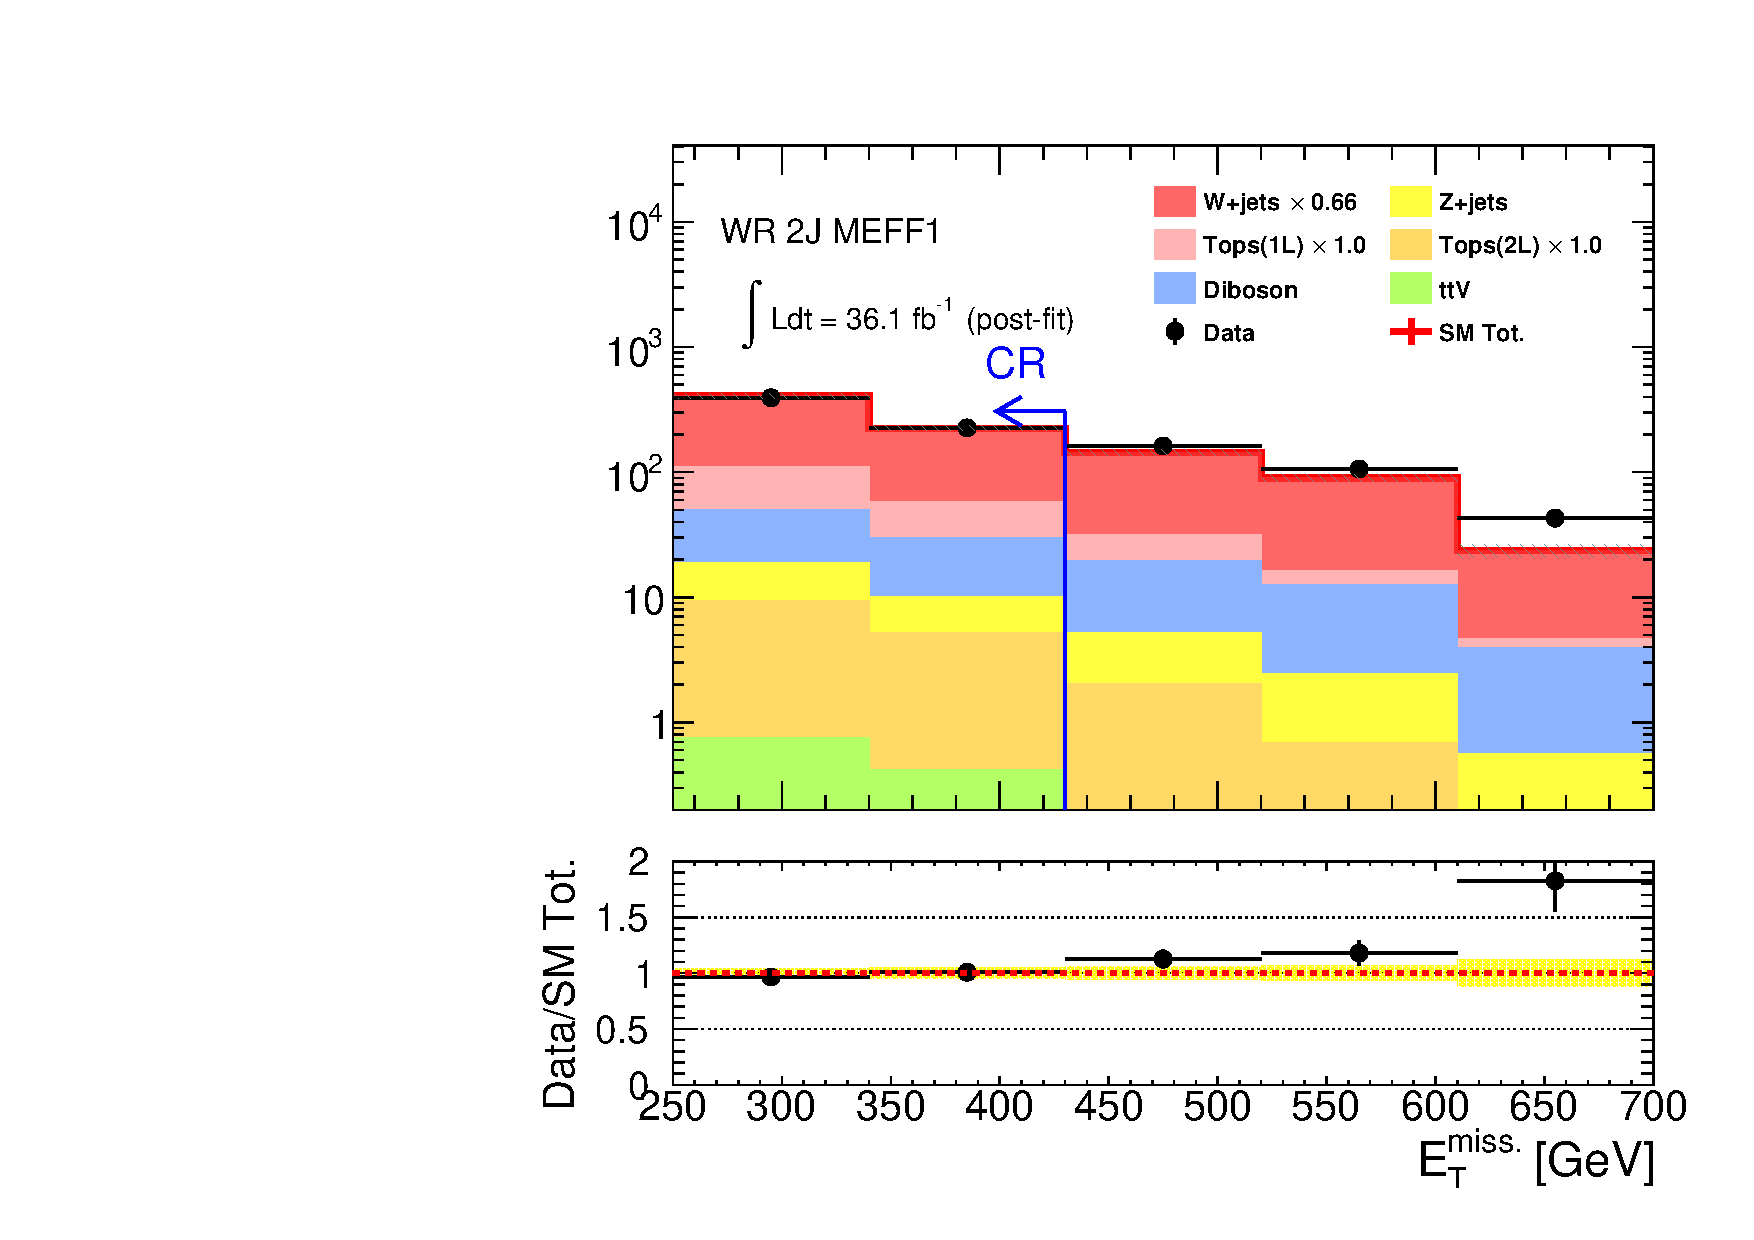
\includegraphics[width=0.41\textwidth]{figures/BGestimation/CRpostFit/WR2JMEFF1/met__WR2JMEFF1_no_met_postFit_2SFconfig_noYields.pdf}}
    \subfigure[]{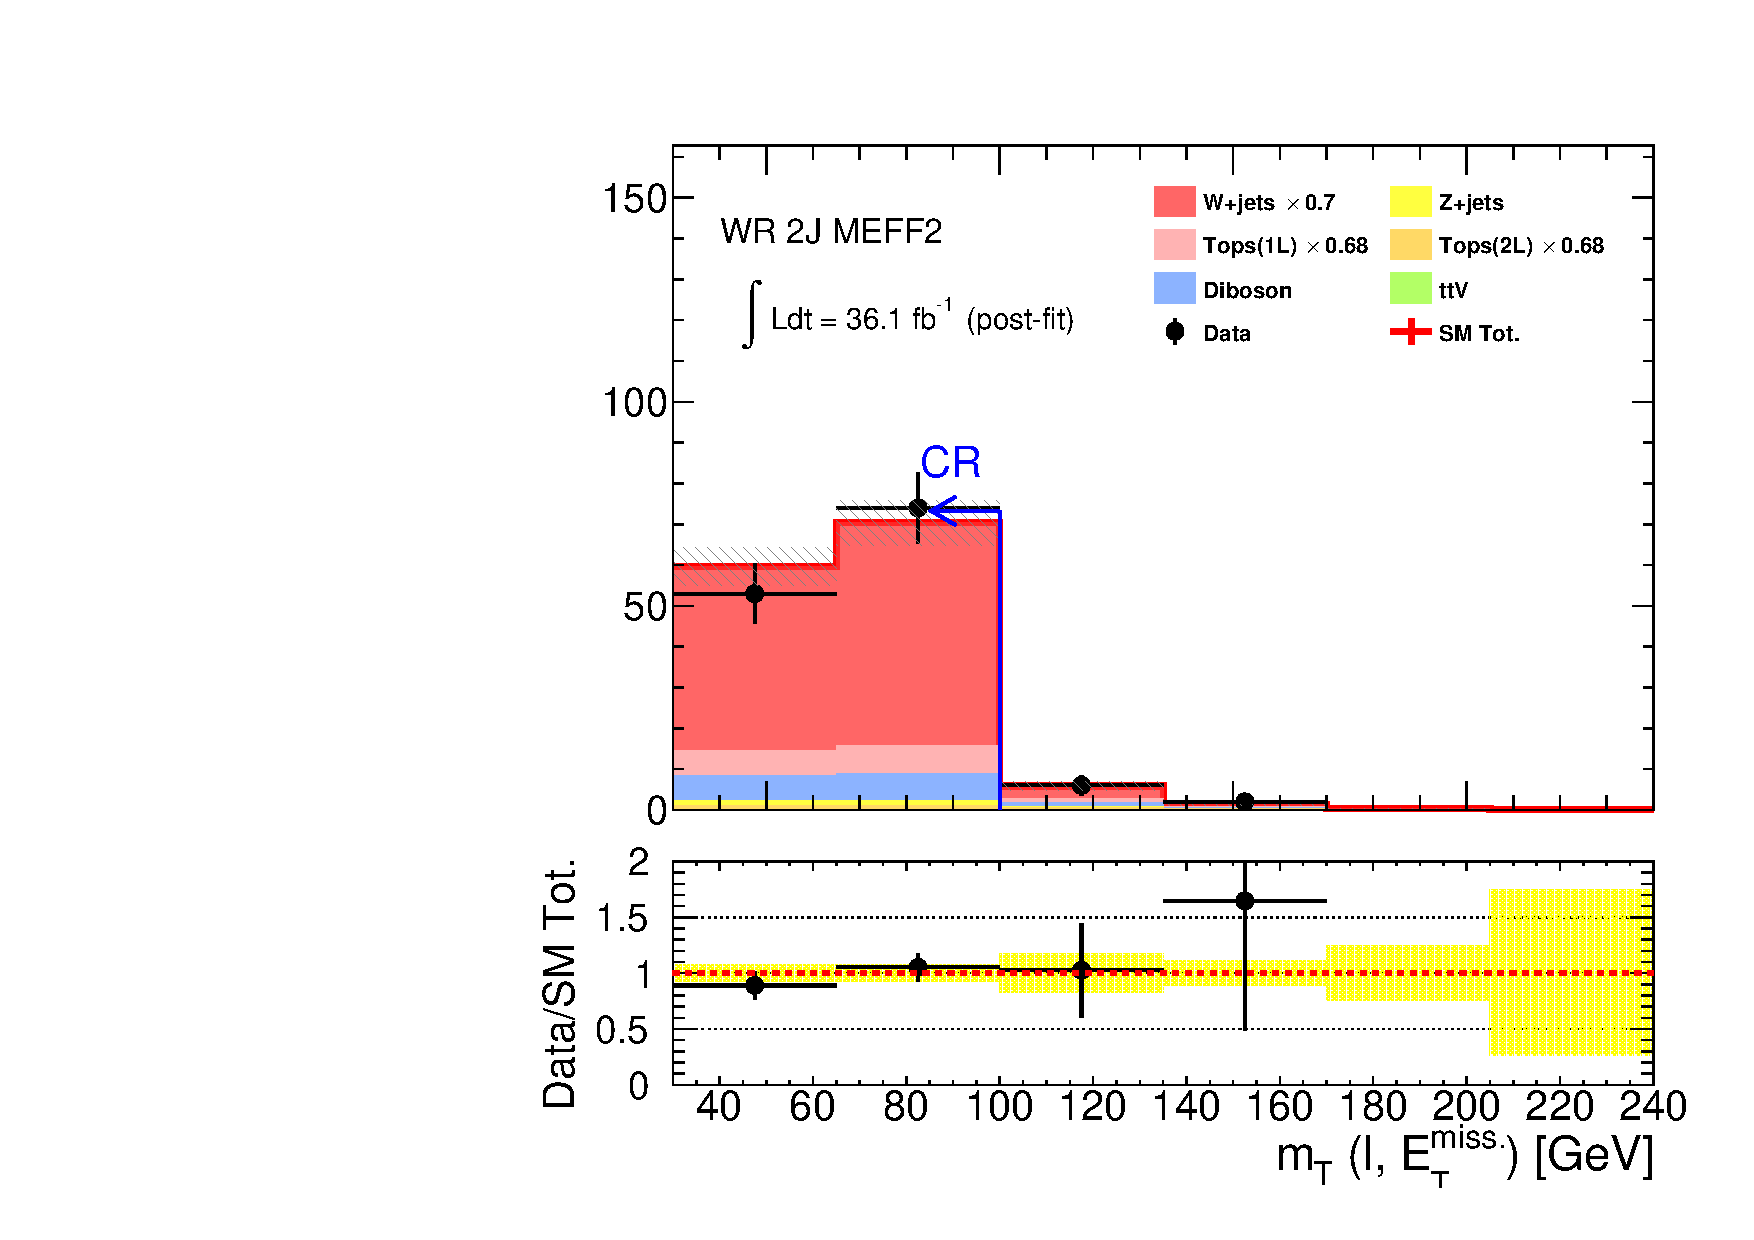
\includegraphics[width=0.41\textwidth]{figures/BGestimation/CRpostFit/WR2JMEFF2/mt__WR2JMEFF2_no_mt_postFit_2SFconfig_noYields.pdf}}
    \subfigure[]{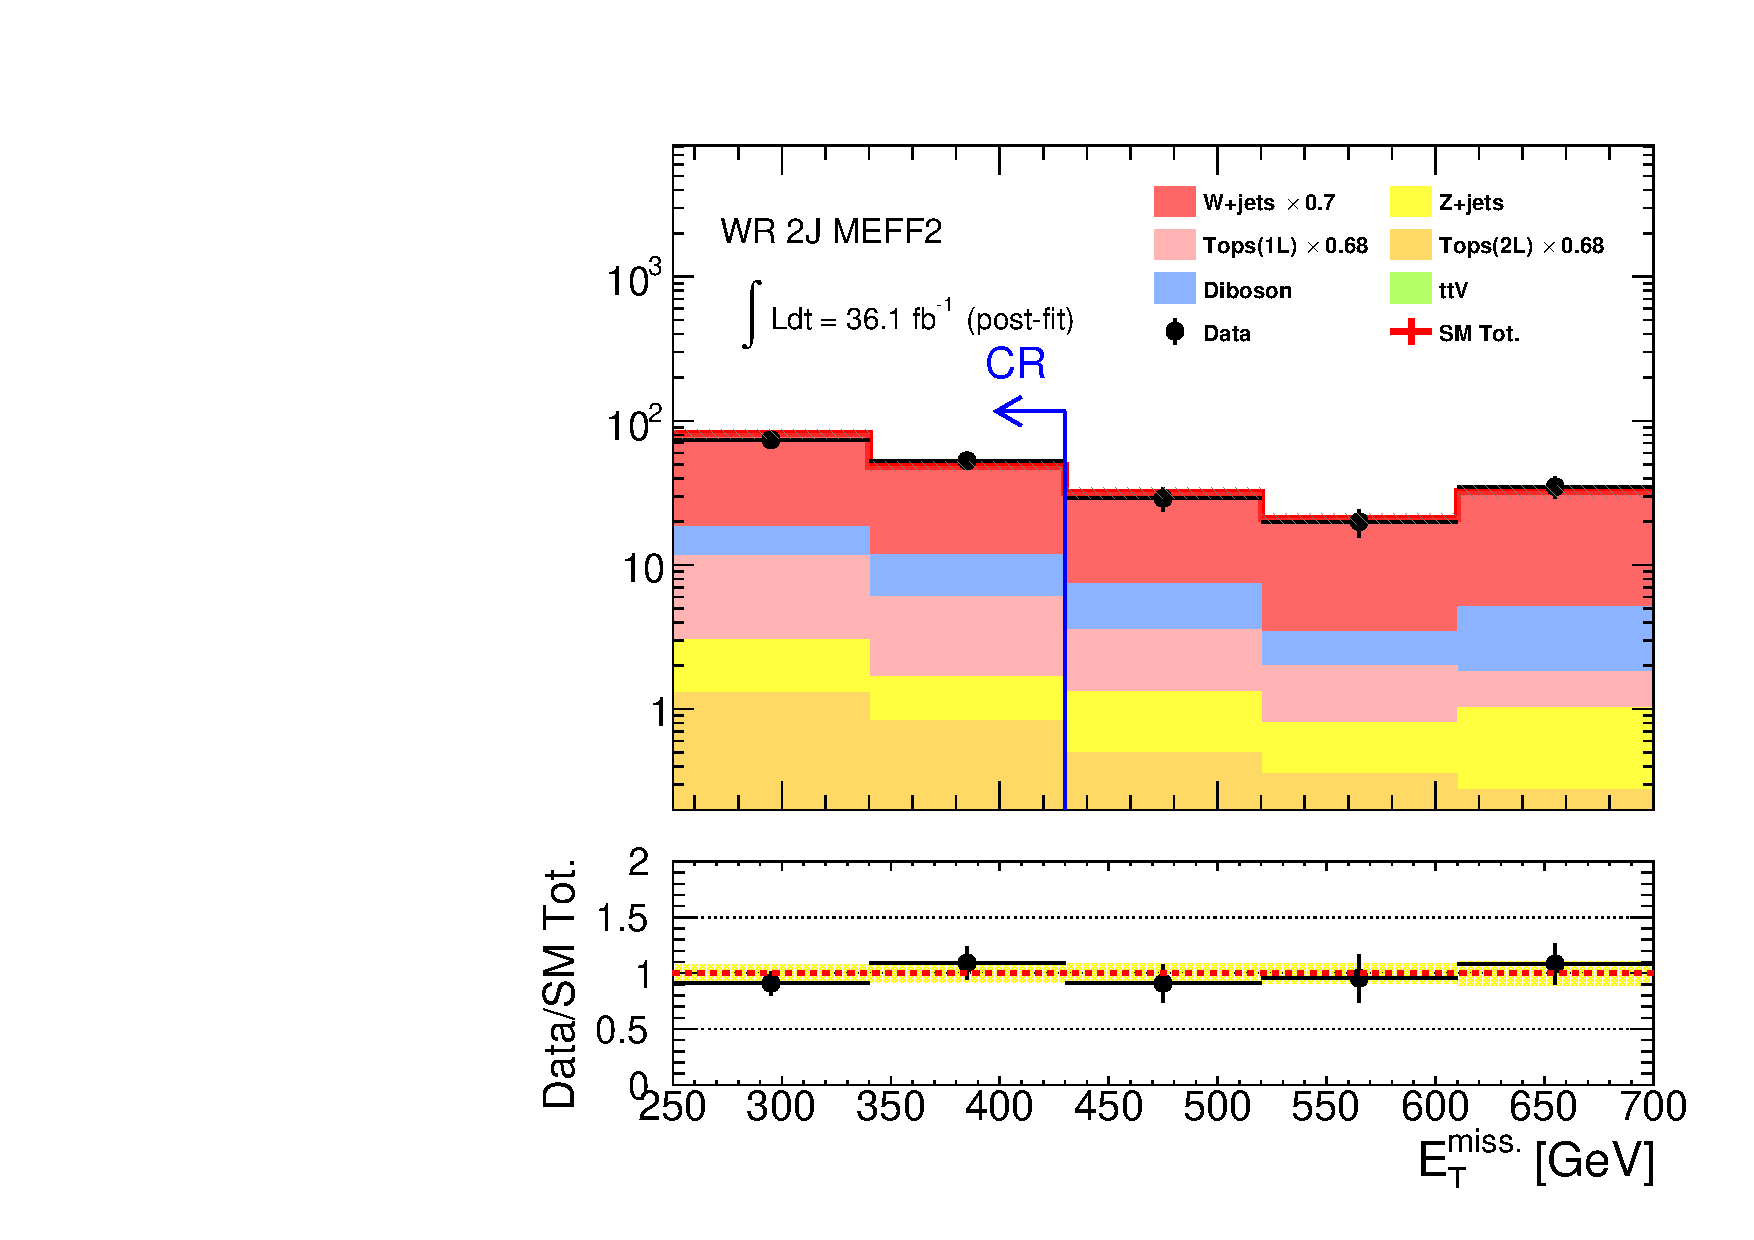
\includegraphics[width=0.41\textwidth]{figures/BGestimation/CRpostFit/WR2JMEFF2/met__WR2JMEFF2_no_met_postFit_2SFconfig_noYields.pdf}}
    \subfigure[]{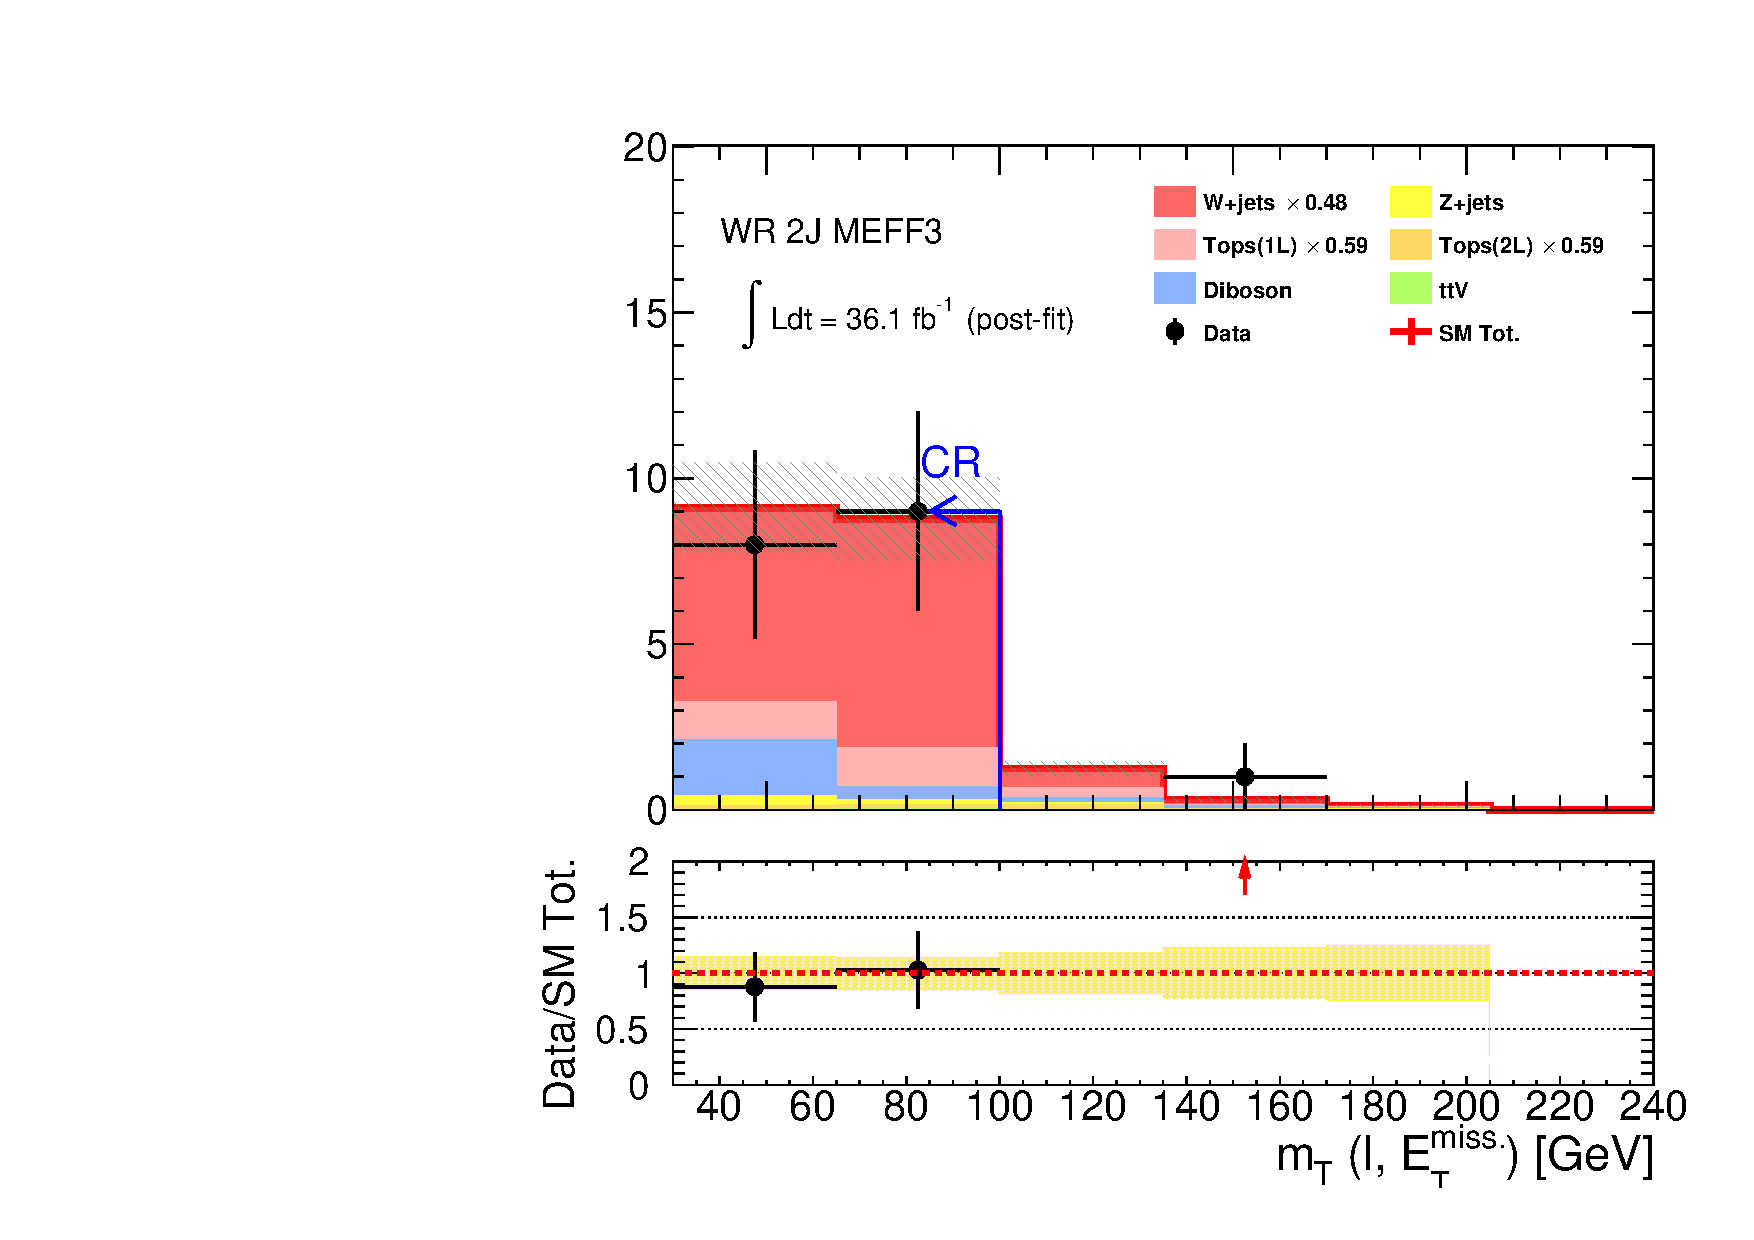
\includegraphics[width=0.41\textwidth]{figures/BGestimation/CRpostFit/WR2JMEFF3/mt__WR2JMEFF3_no_mt_postFit_2SFconfig_noYields.pdf}}
    \subfigure[]{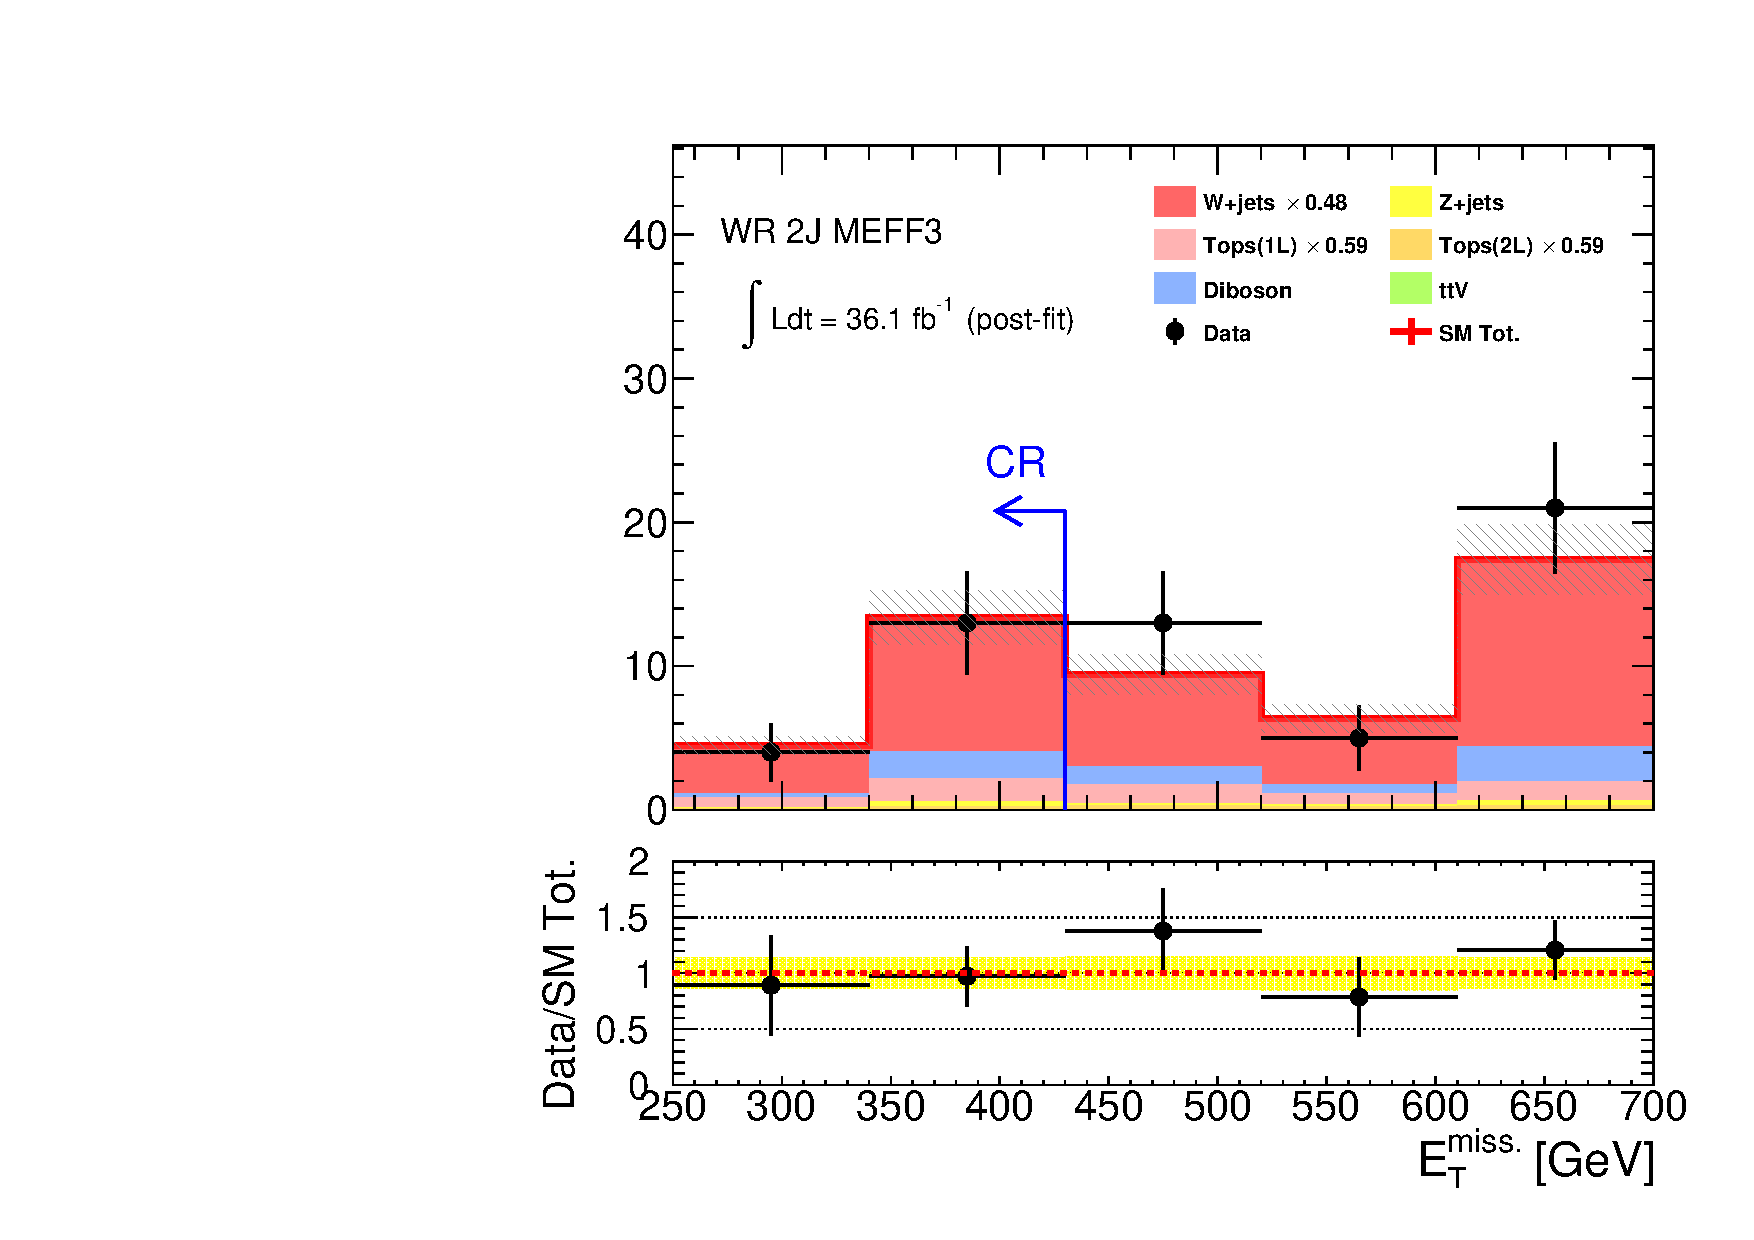
\includegraphics[width=0.41\textwidth]{figures/BGestimation/CRpostFit/WR2JMEFF3/met__WR2JMEFF3_no_met_postFit_2SFconfig_noYields.pdf}}
   \caption{
     Post-fit distruibution of (left) $\mt$ (right) $\met$.
     (a,b) WR 2J-$\meffIncFirst$.
     (c,d) WR 2J-$\meffIncSecond$.
     (e,f) WR 2J-$\meffIncThird$. 
     The yellow band in the bottom panel represents only statistical error. The overflow is included in the highest bin.  
   \label{fig::BGestimation::CRpostFit::WR2J}}    
\end{figure}
%----------------------------------
\clearpage
\begin{figure}[h]
  \centering
    \subfigure[]{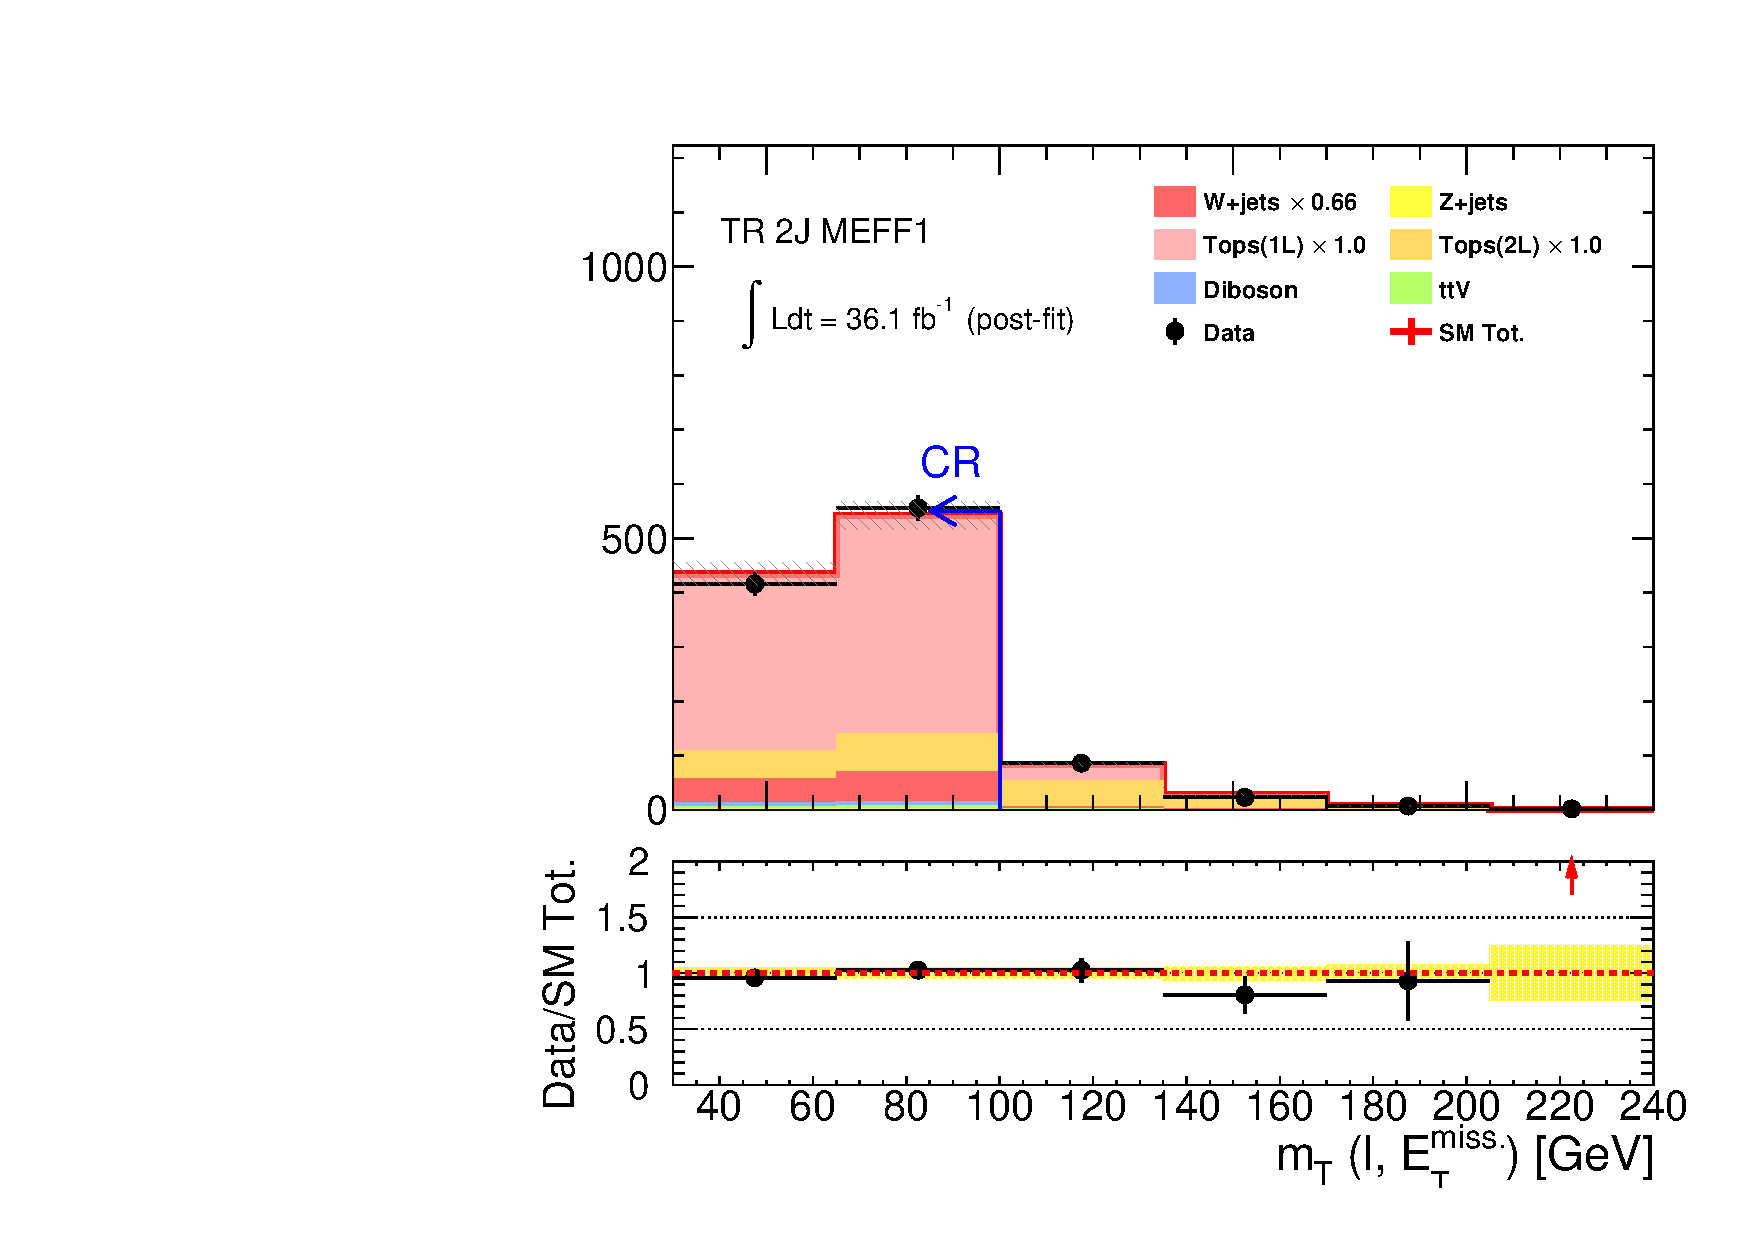
\includegraphics[width=0.41\textwidth]{figures/BGestimation/CRpostFit/TR2JMEFF1/mt__TR2JMEFF1_no_mt_postFit_2SFconfig_noYields.pdf}}
    \subfigure[]{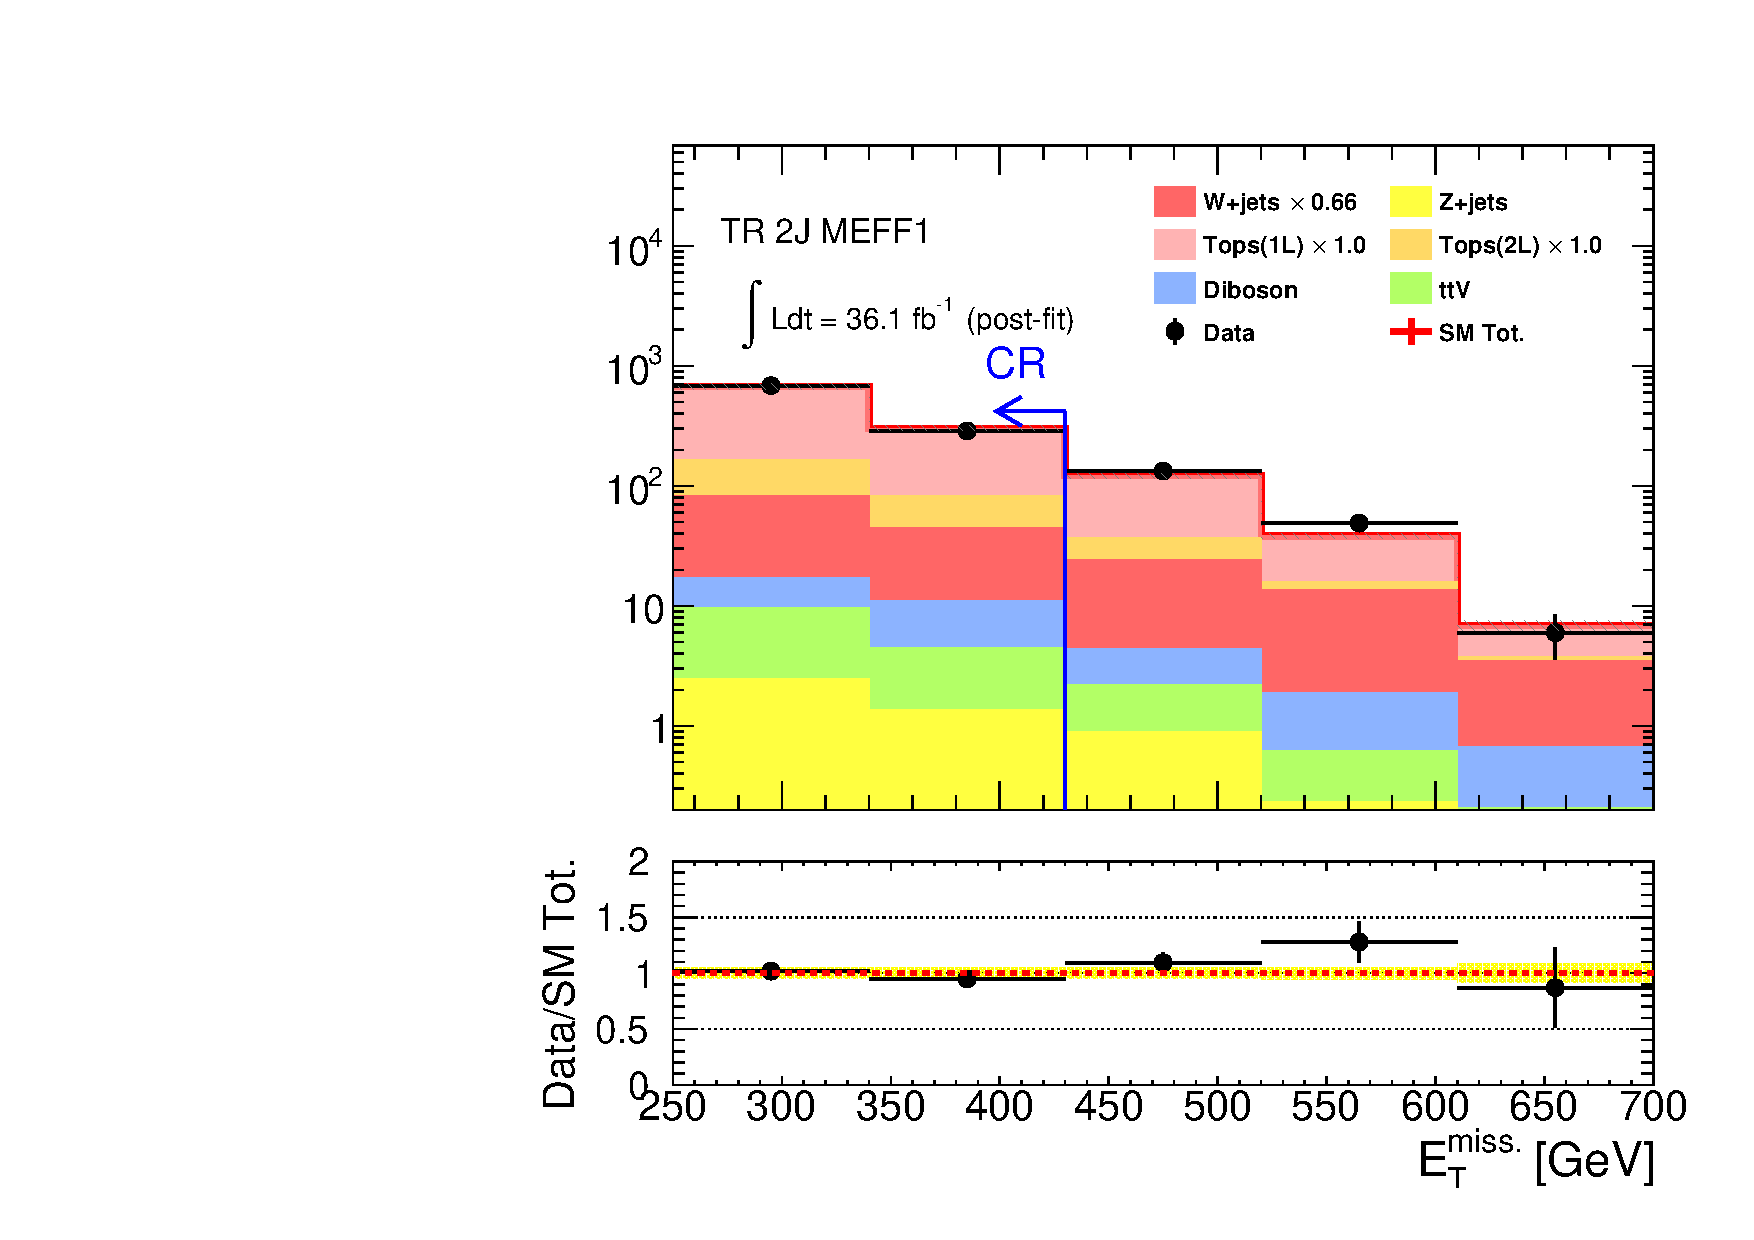
\includegraphics[width=0.41\textwidth]{figures/BGestimation/CRpostFit/TR2JMEFF1/met__TR2JMEFF1_no_met_postFit_2SFconfig_noYields.pdf}}
    \subfigure[]{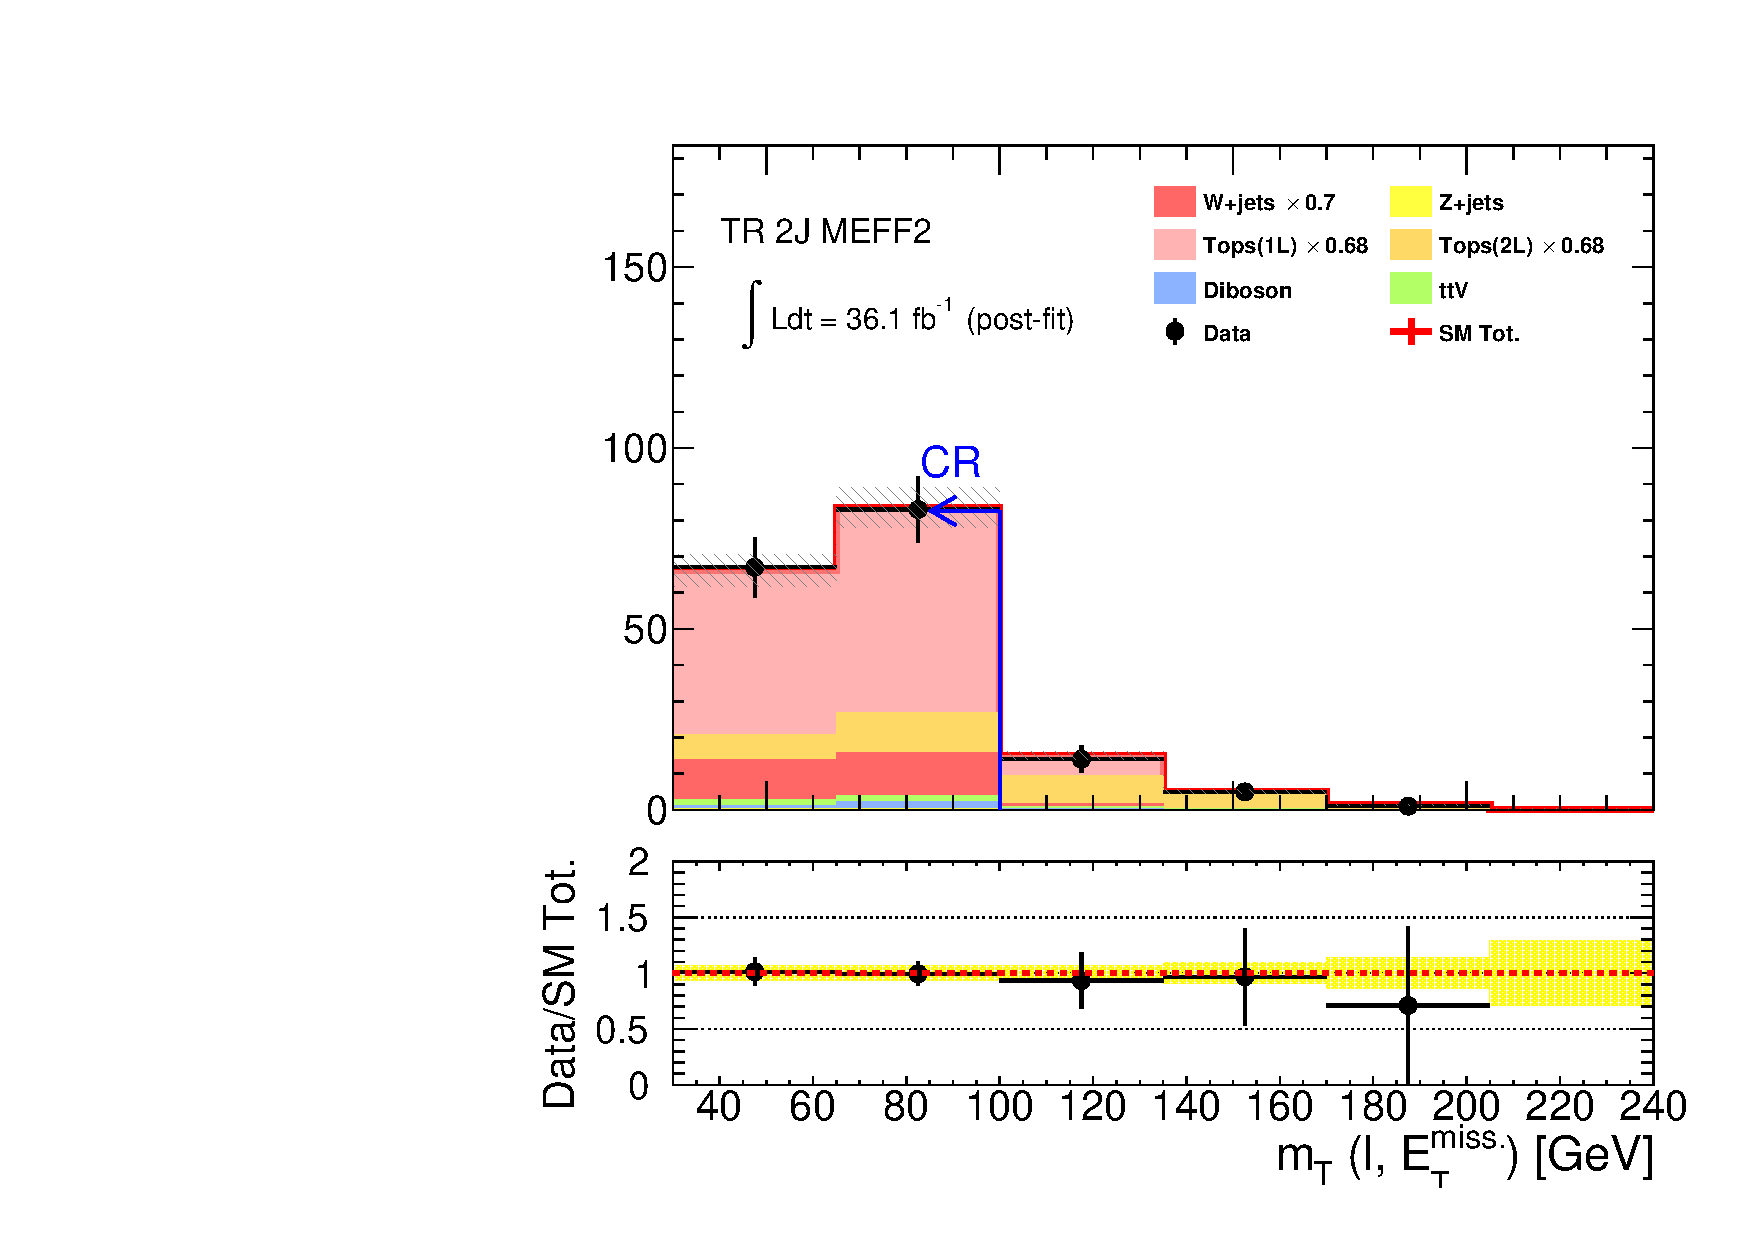
\includegraphics[width=0.41\textwidth]{figures/BGestimation/CRpostFit/TR2JMEFF2/mt__TR2JMEFF2_no_mt_postFit_2SFconfig_noYields.pdf}}
    \subfigure[]{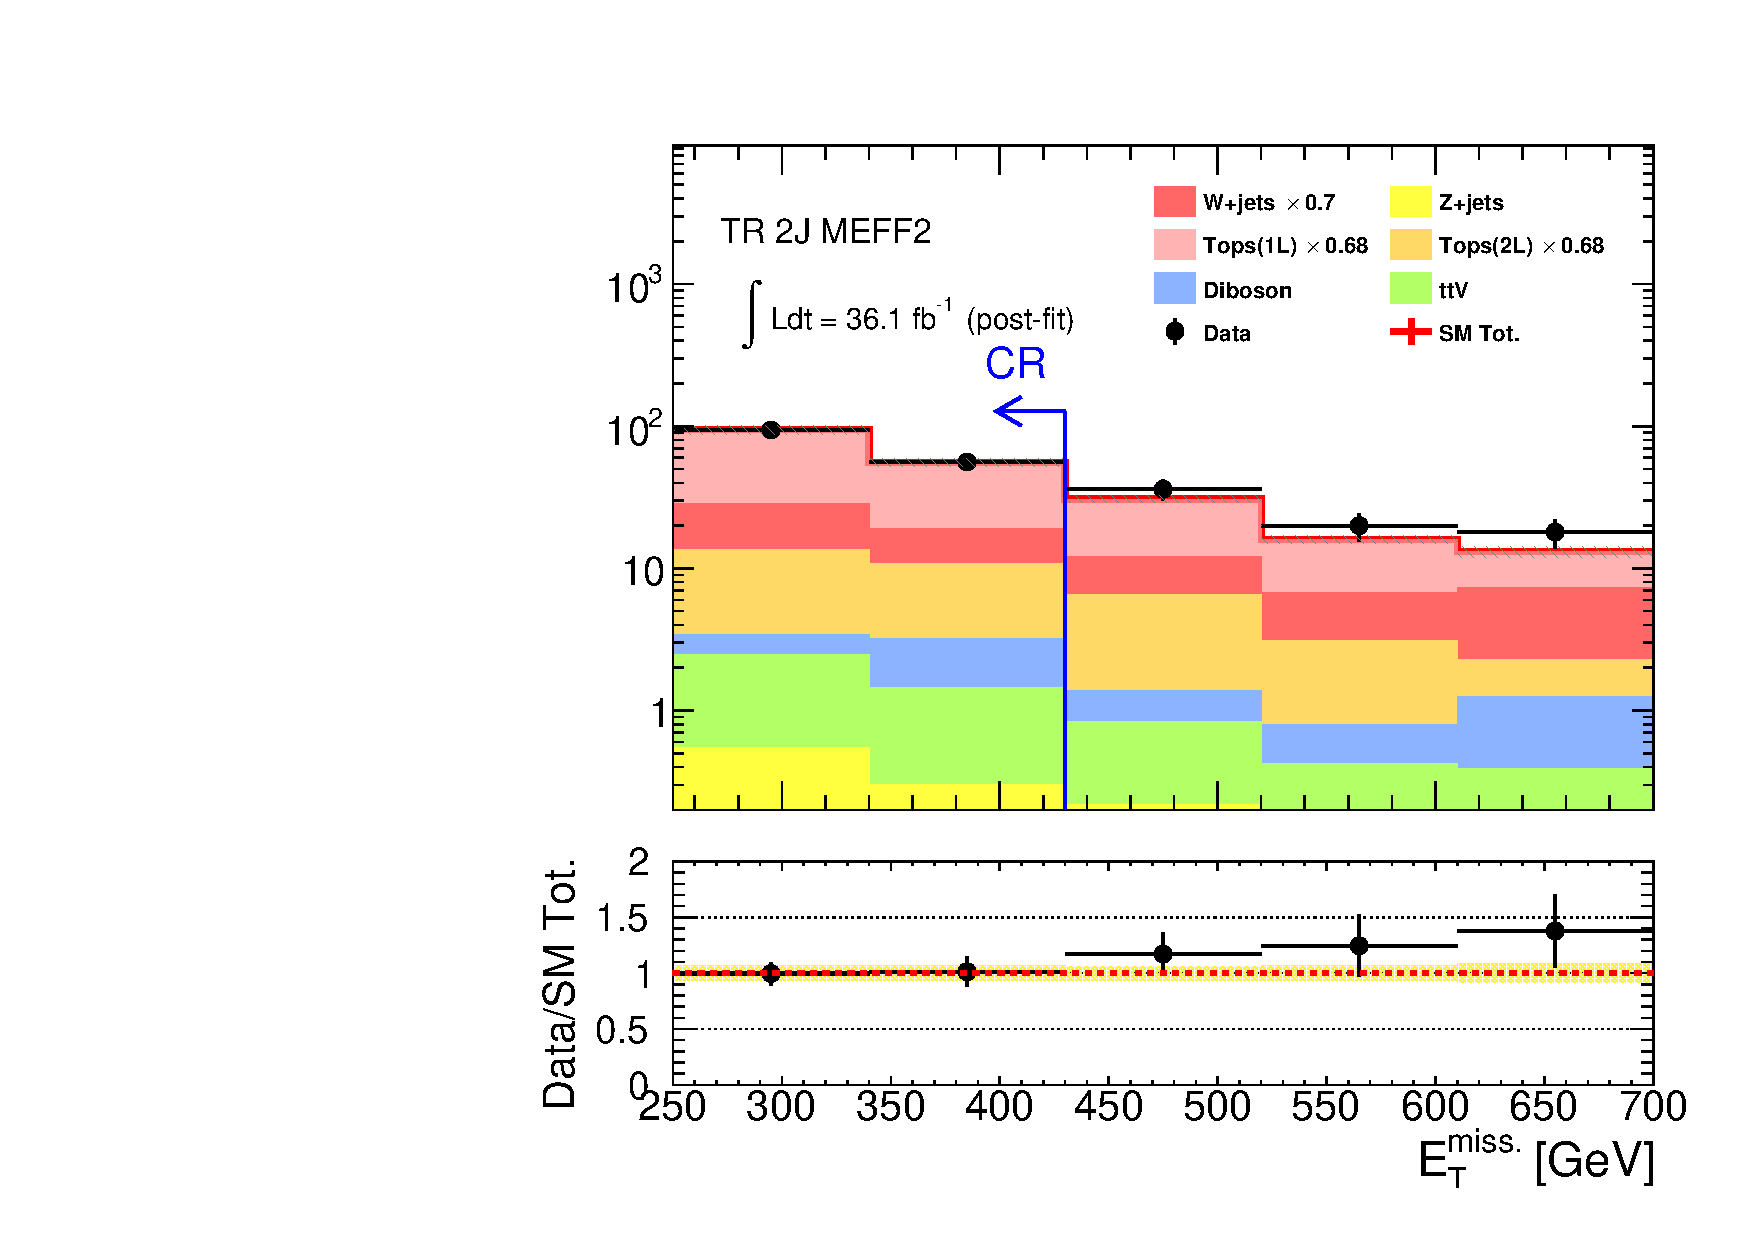
\includegraphics[width=0.41\textwidth]{figures/BGestimation/CRpostFit/TR2JMEFF2/met__TR2JMEFF2_no_met_postFit_2SFconfig_noYields.pdf}}
    \subfigure[]{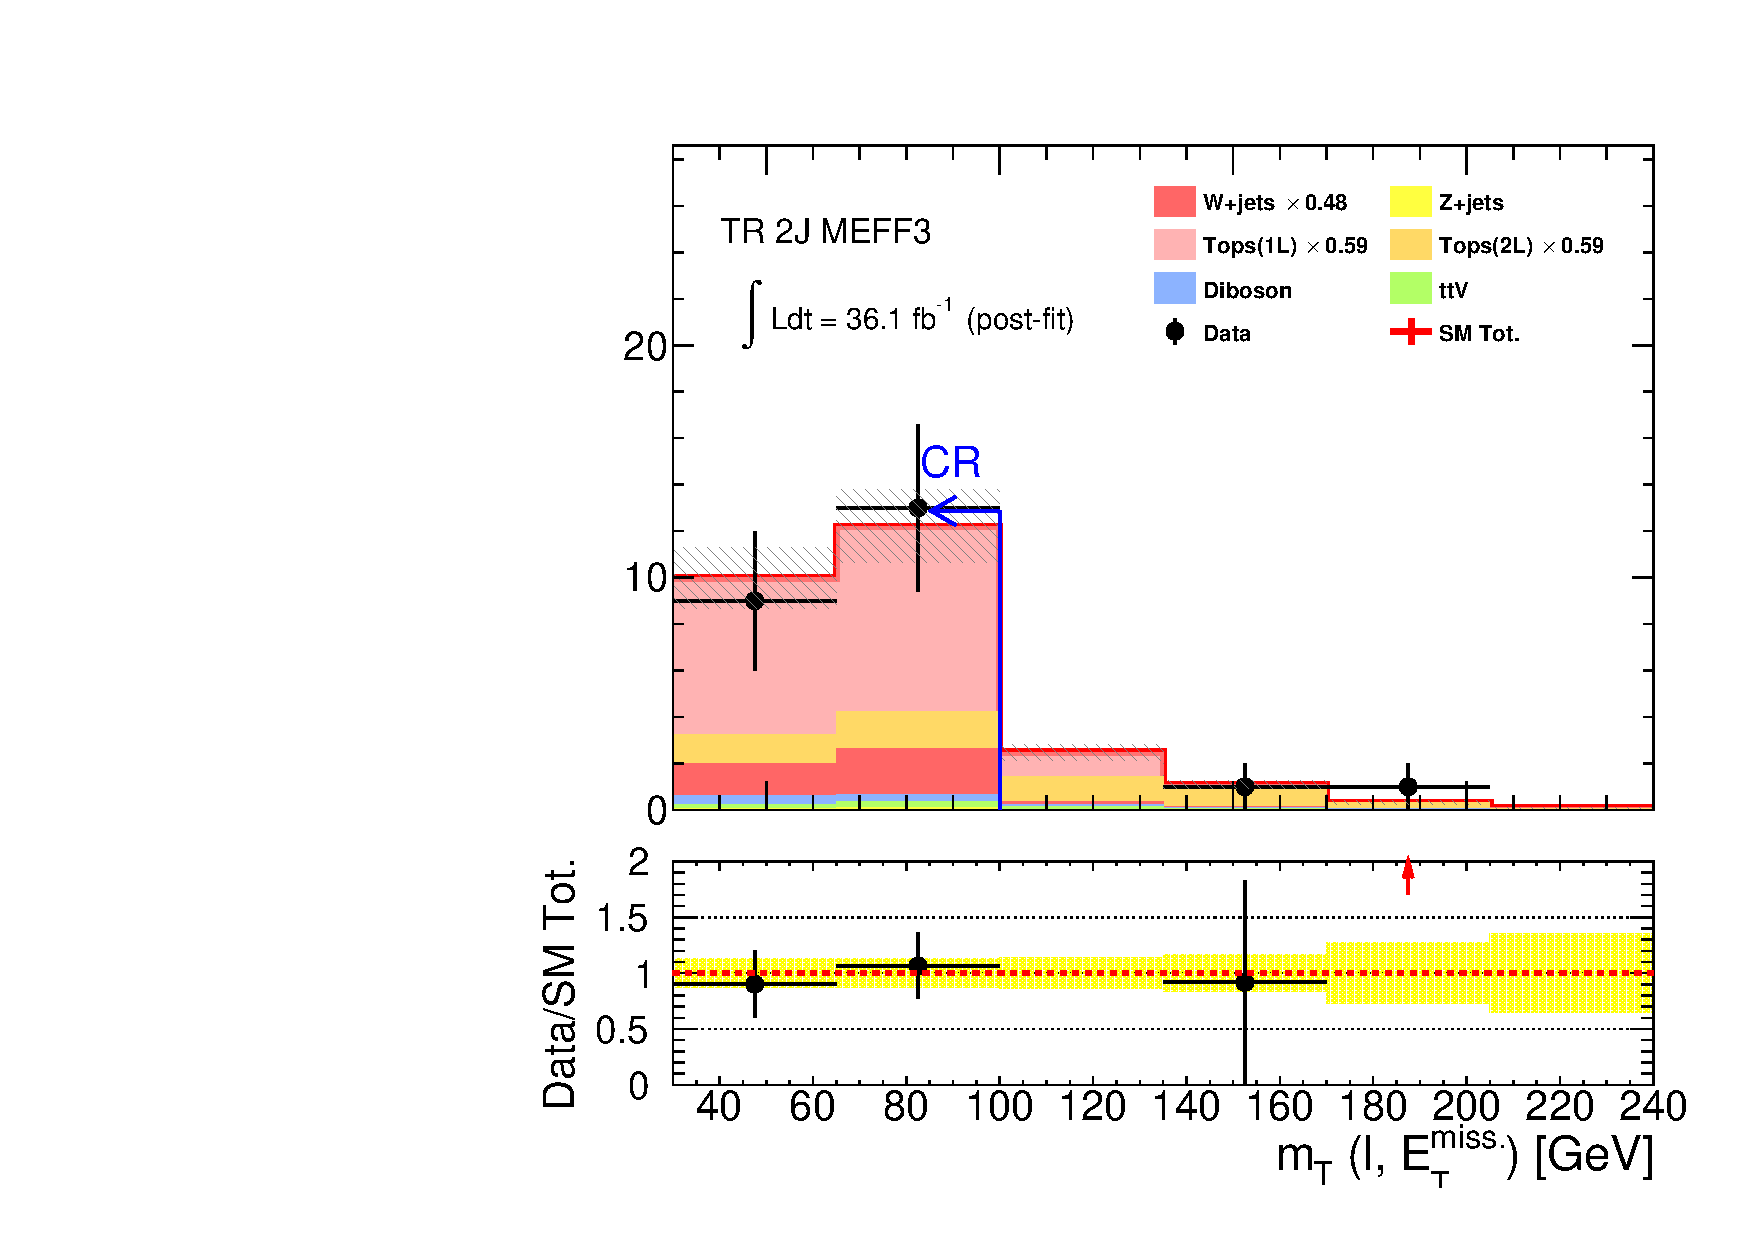
\includegraphics[width=0.41\textwidth]{figures/BGestimation/CRpostFit/TR2JMEFF3/mt__TR2JMEFF3_no_mt_postFit_2SFconfig_noYields.pdf}}
    \subfigure[]{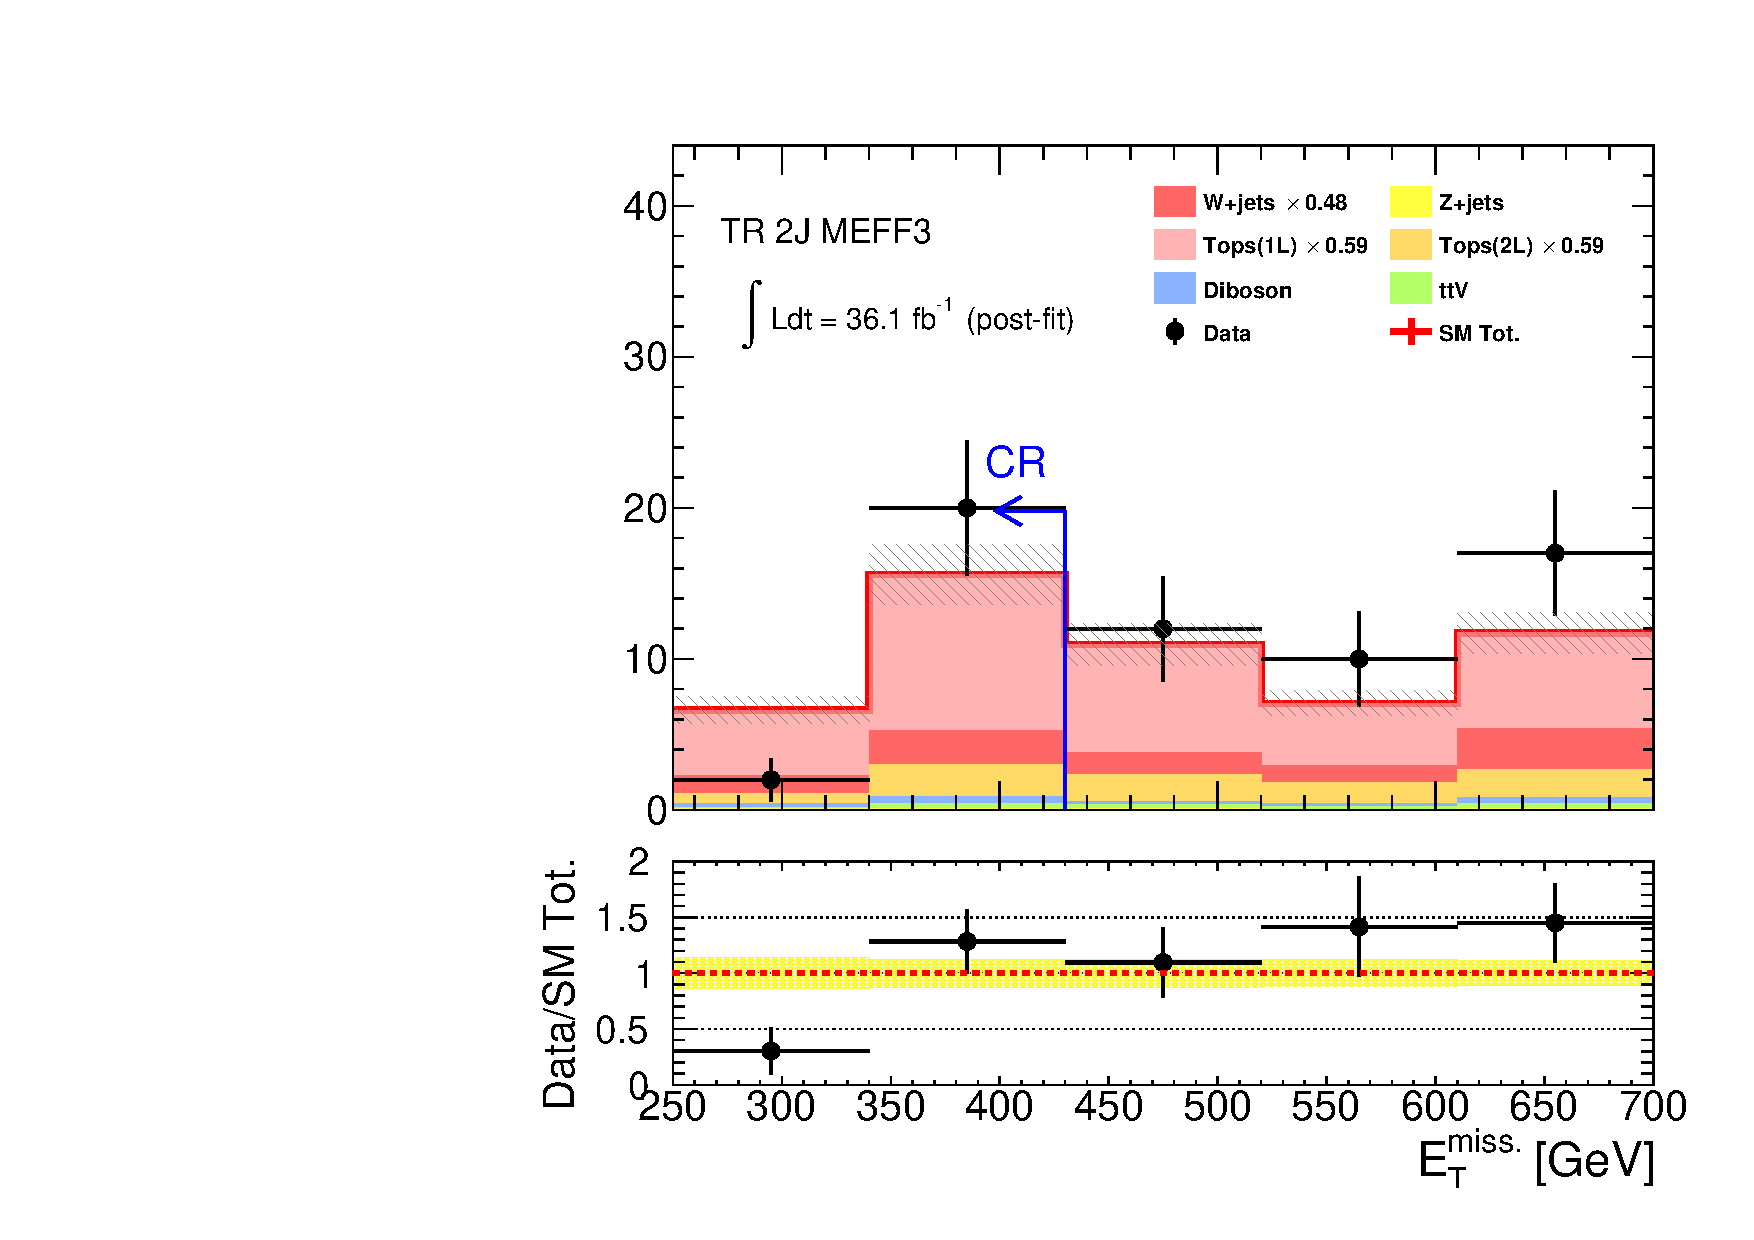
\includegraphics[width=0.41\textwidth]{figures/BGestimation/CRpostFit/TR2JMEFF3/met__TR2JMEFF3_no_met_postFit_2SFconfig_noYields.pdf}}
   \caption{
     Post-fit distruibution of (left) $\mt$ (right) $\met$.
     (a,b) TR 2J-$\meffIncFirst$. 
     (c,d) TR 2J-$\meffIncSecond$.
     (e,f) TR 2J-$\meffIncThird$.
     The yellow band in the bottom panel represents only statistical error. The overflow is included in the highest bin.  
   \label{fig::BGestimation::CRpostFit::TR2J}}    
\end{figure}
%----------------------------------

\clearpage
% -------------- 6J ---------
\begin{figure}[h]
  \centering
    \subfigure[]{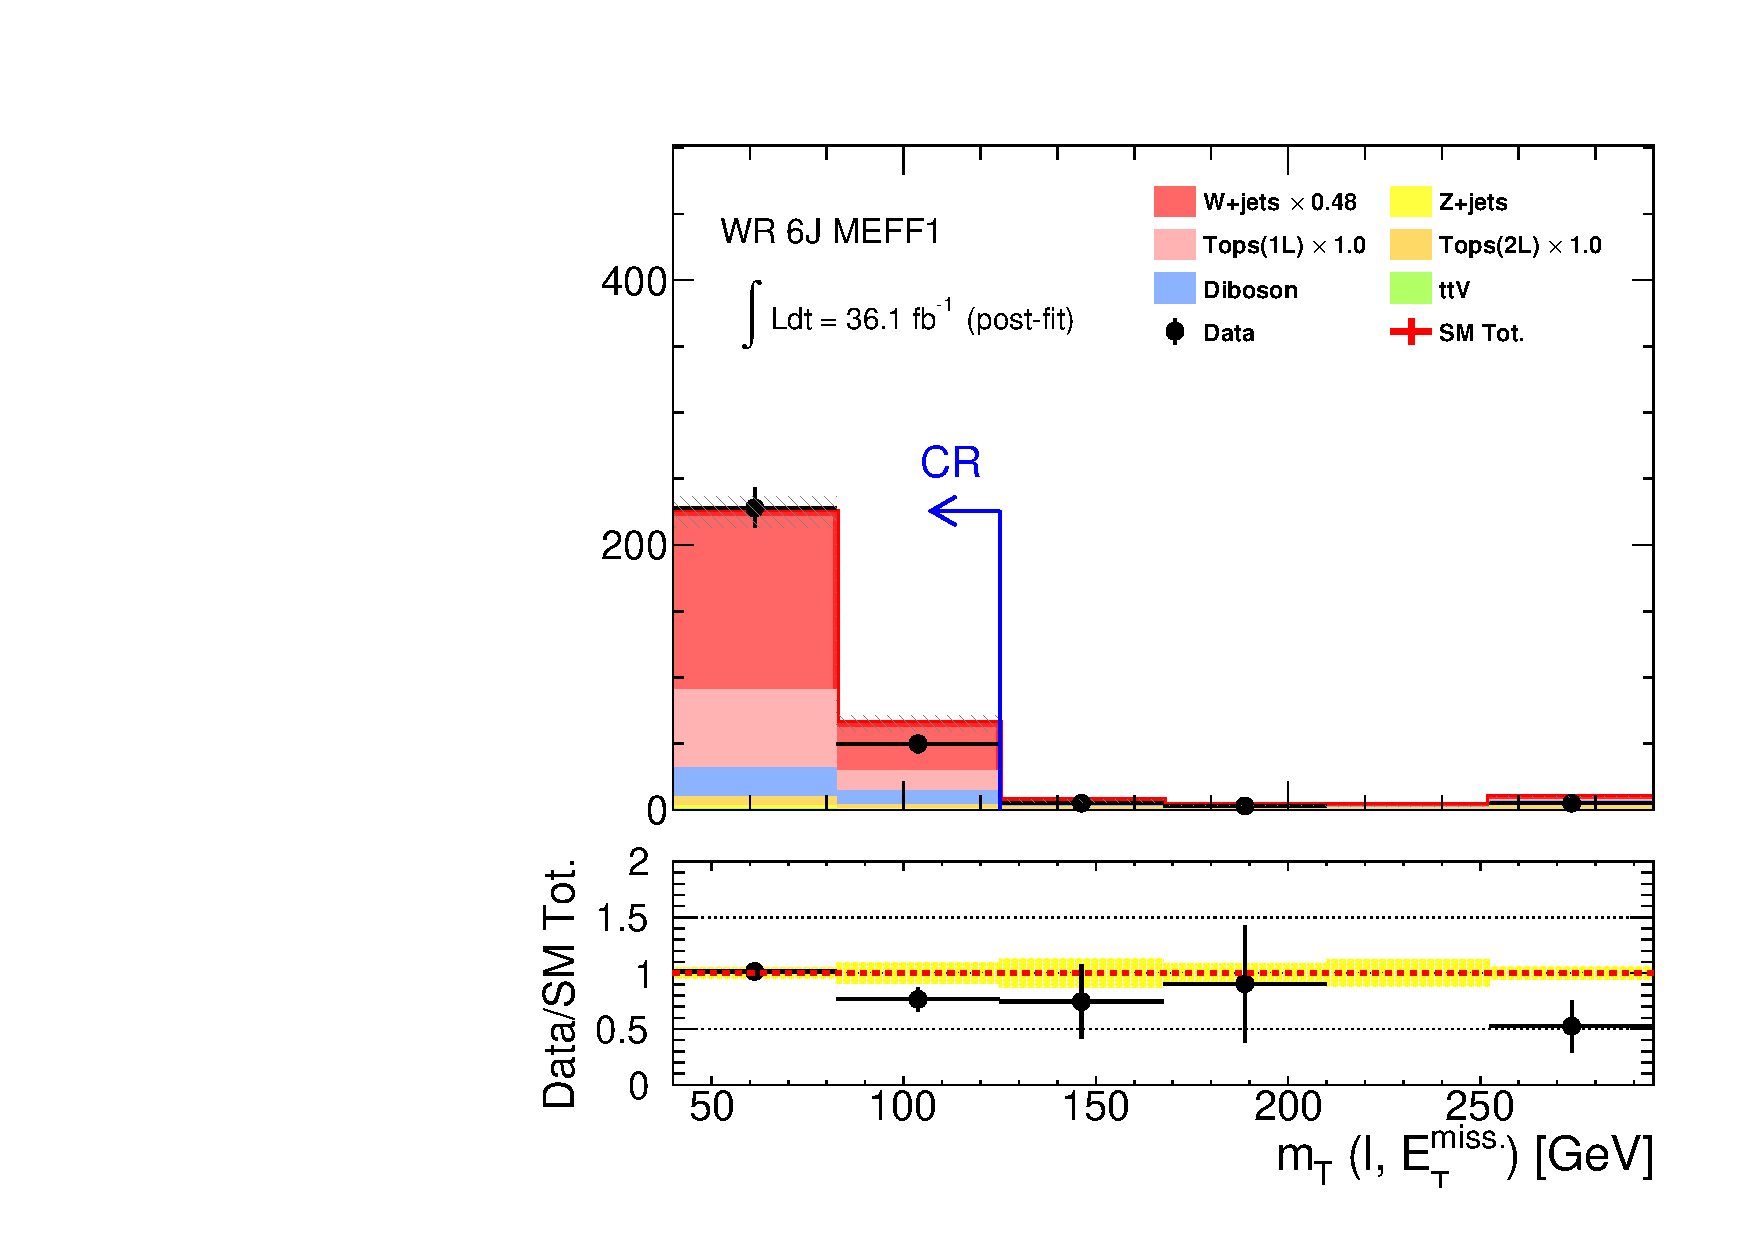
\includegraphics[width=0.41\textwidth]{figures/BGestimation/CRpostFit/WR6JMEFF1/mt__WR6JMEFF1_no_mt_postFit_2SFconfig_noYields.pdf}}
    \subfigure[]{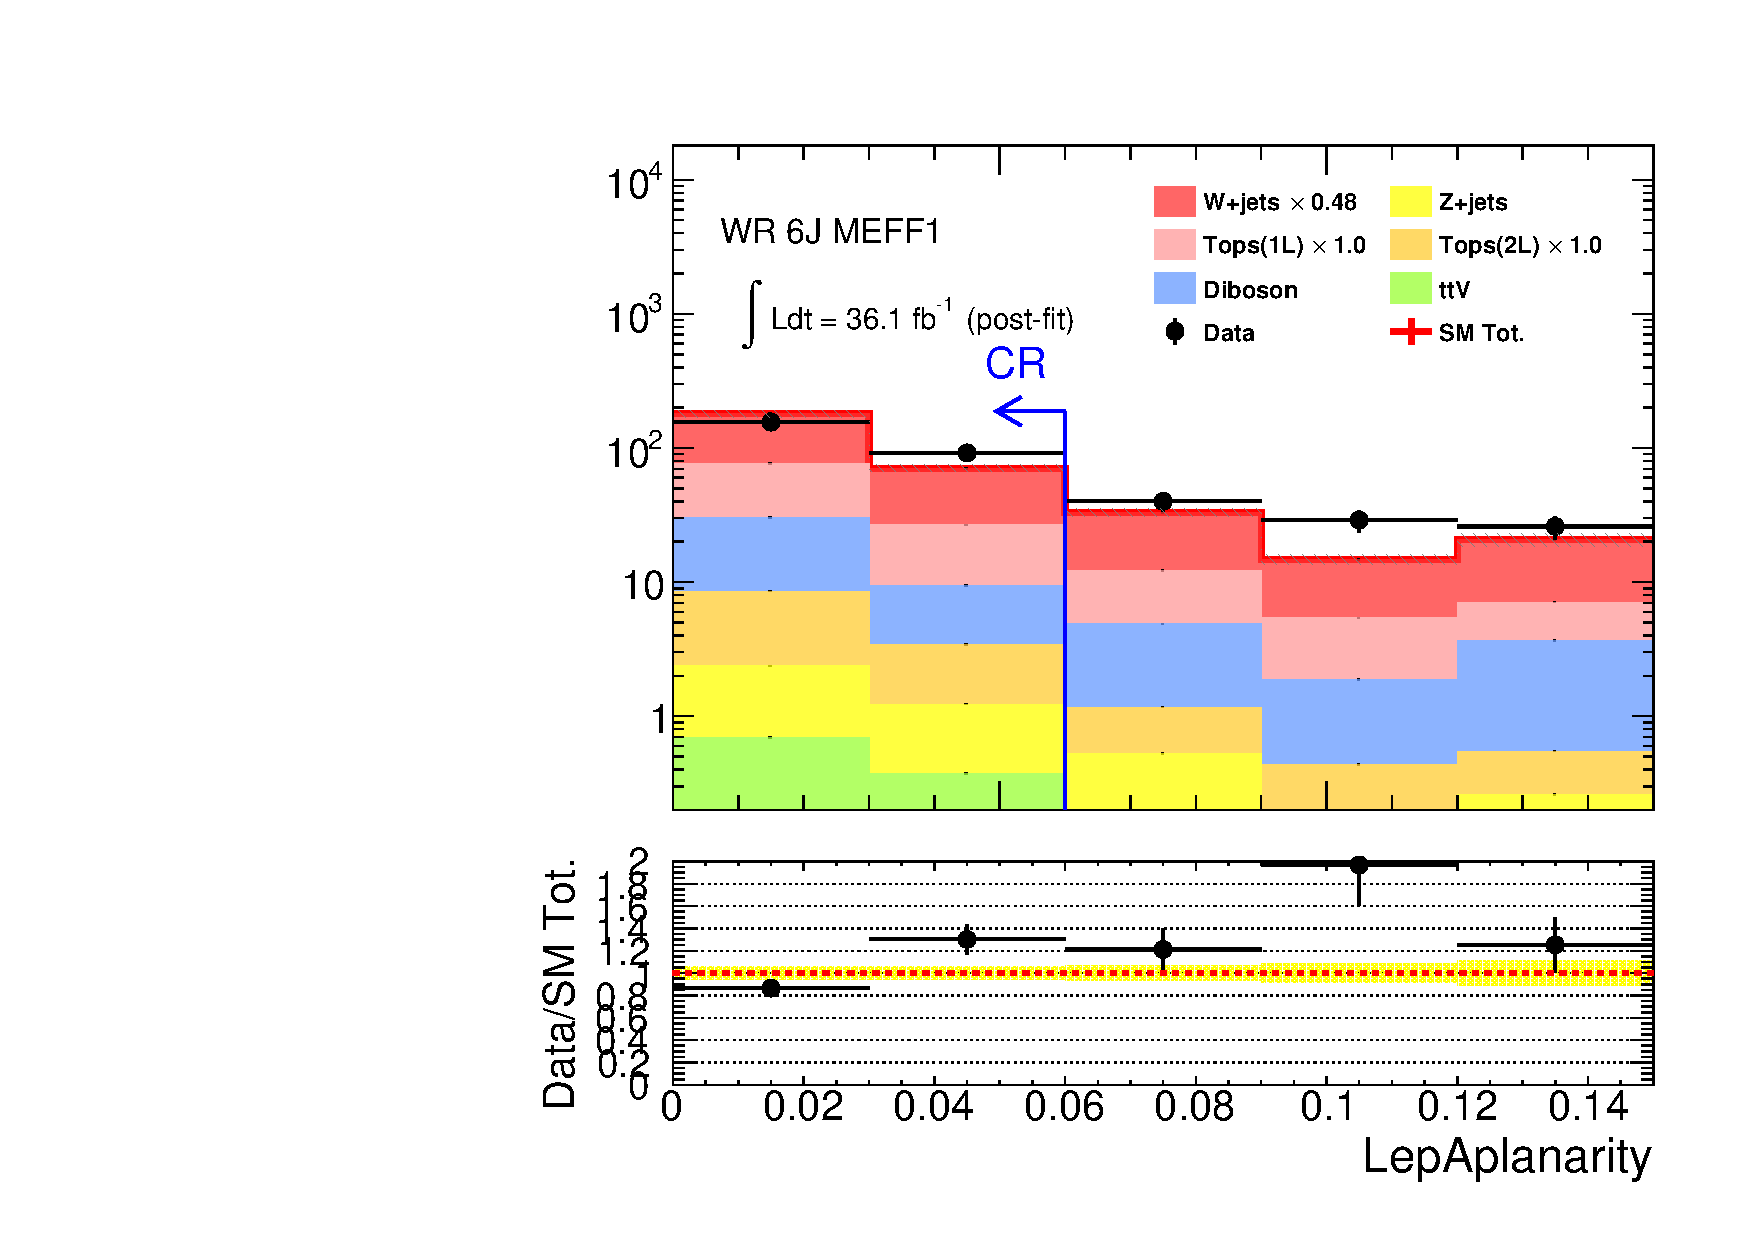
\includegraphics[width=0.41\textwidth]{figures/BGestimation/CRpostFit/WR6JMEFF1/LepAplanarity__WR6JMEFF1_no_LepAplanarity_postFit_2SFconfig_noYields.pdf}}
    \subfigure[]{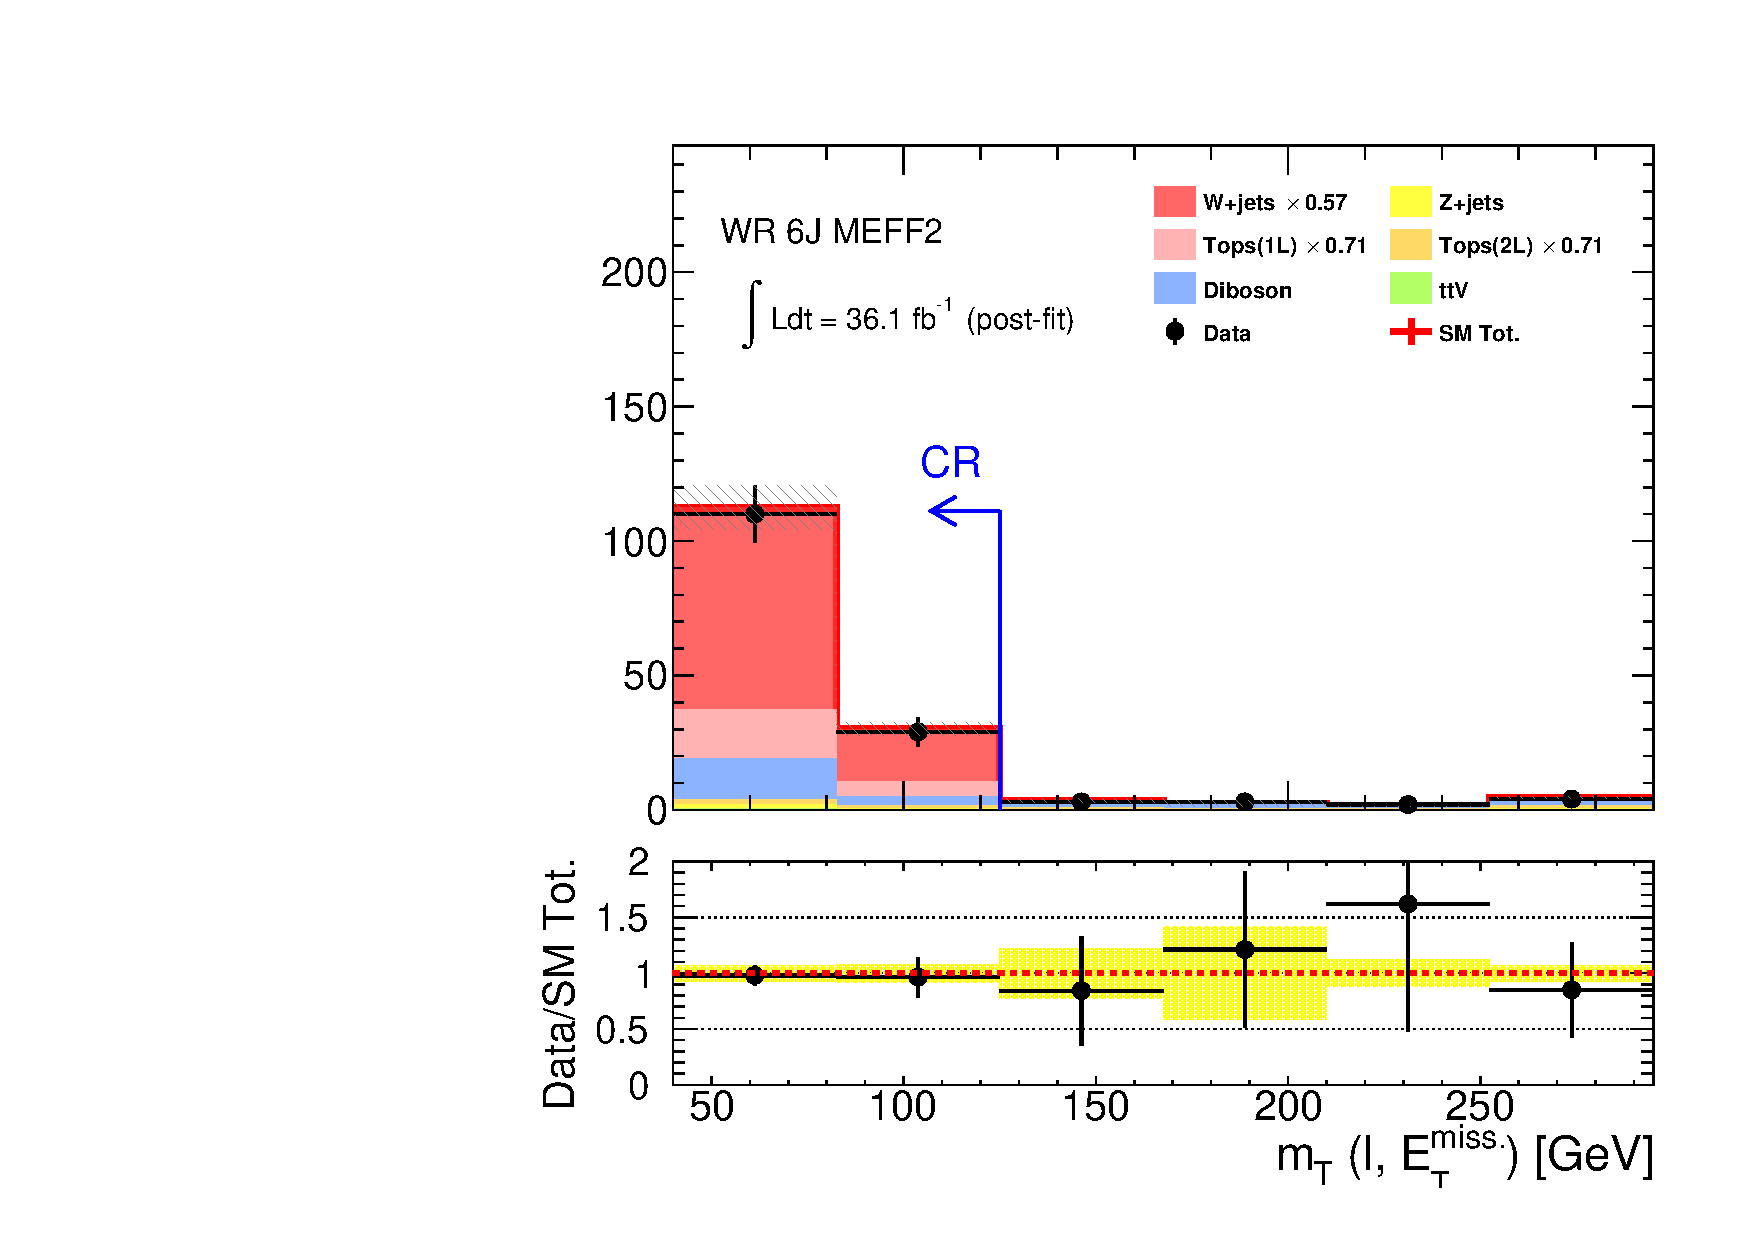
\includegraphics[width=0.41\textwidth]{figures/BGestimation/CRpostFit/WR6JMEFF2/mt__WR6JMEFF2_no_mt_postFit_2SFconfig_noYields.pdf}}
    \subfigure[]{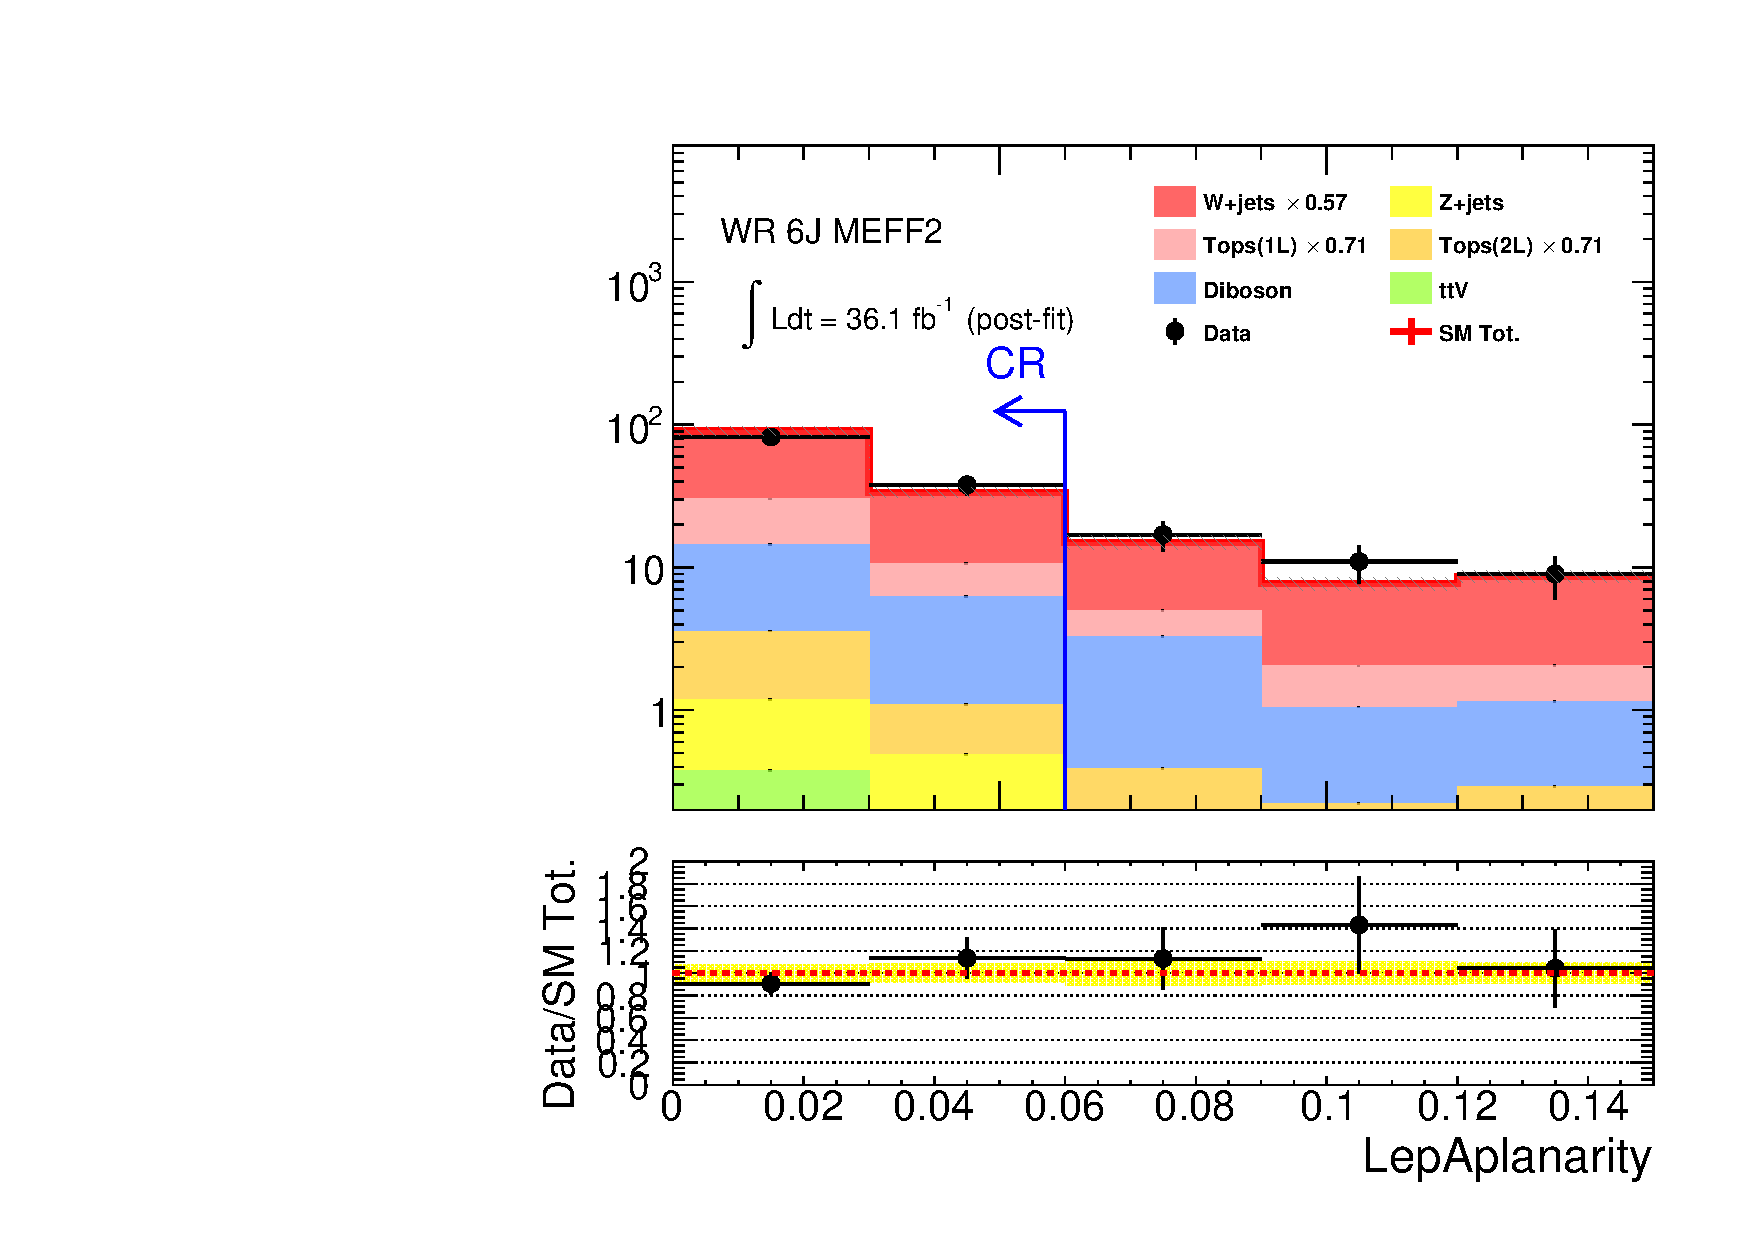
\includegraphics[width=0.41\textwidth]{figures/BGestimation/CRpostFit/WR6JMEFF2/LepAplanarity__WR6JMEFF2_no_LepAplanarity_postFit_2SFconfig_noYields.pdf}}
    \subfigure[]{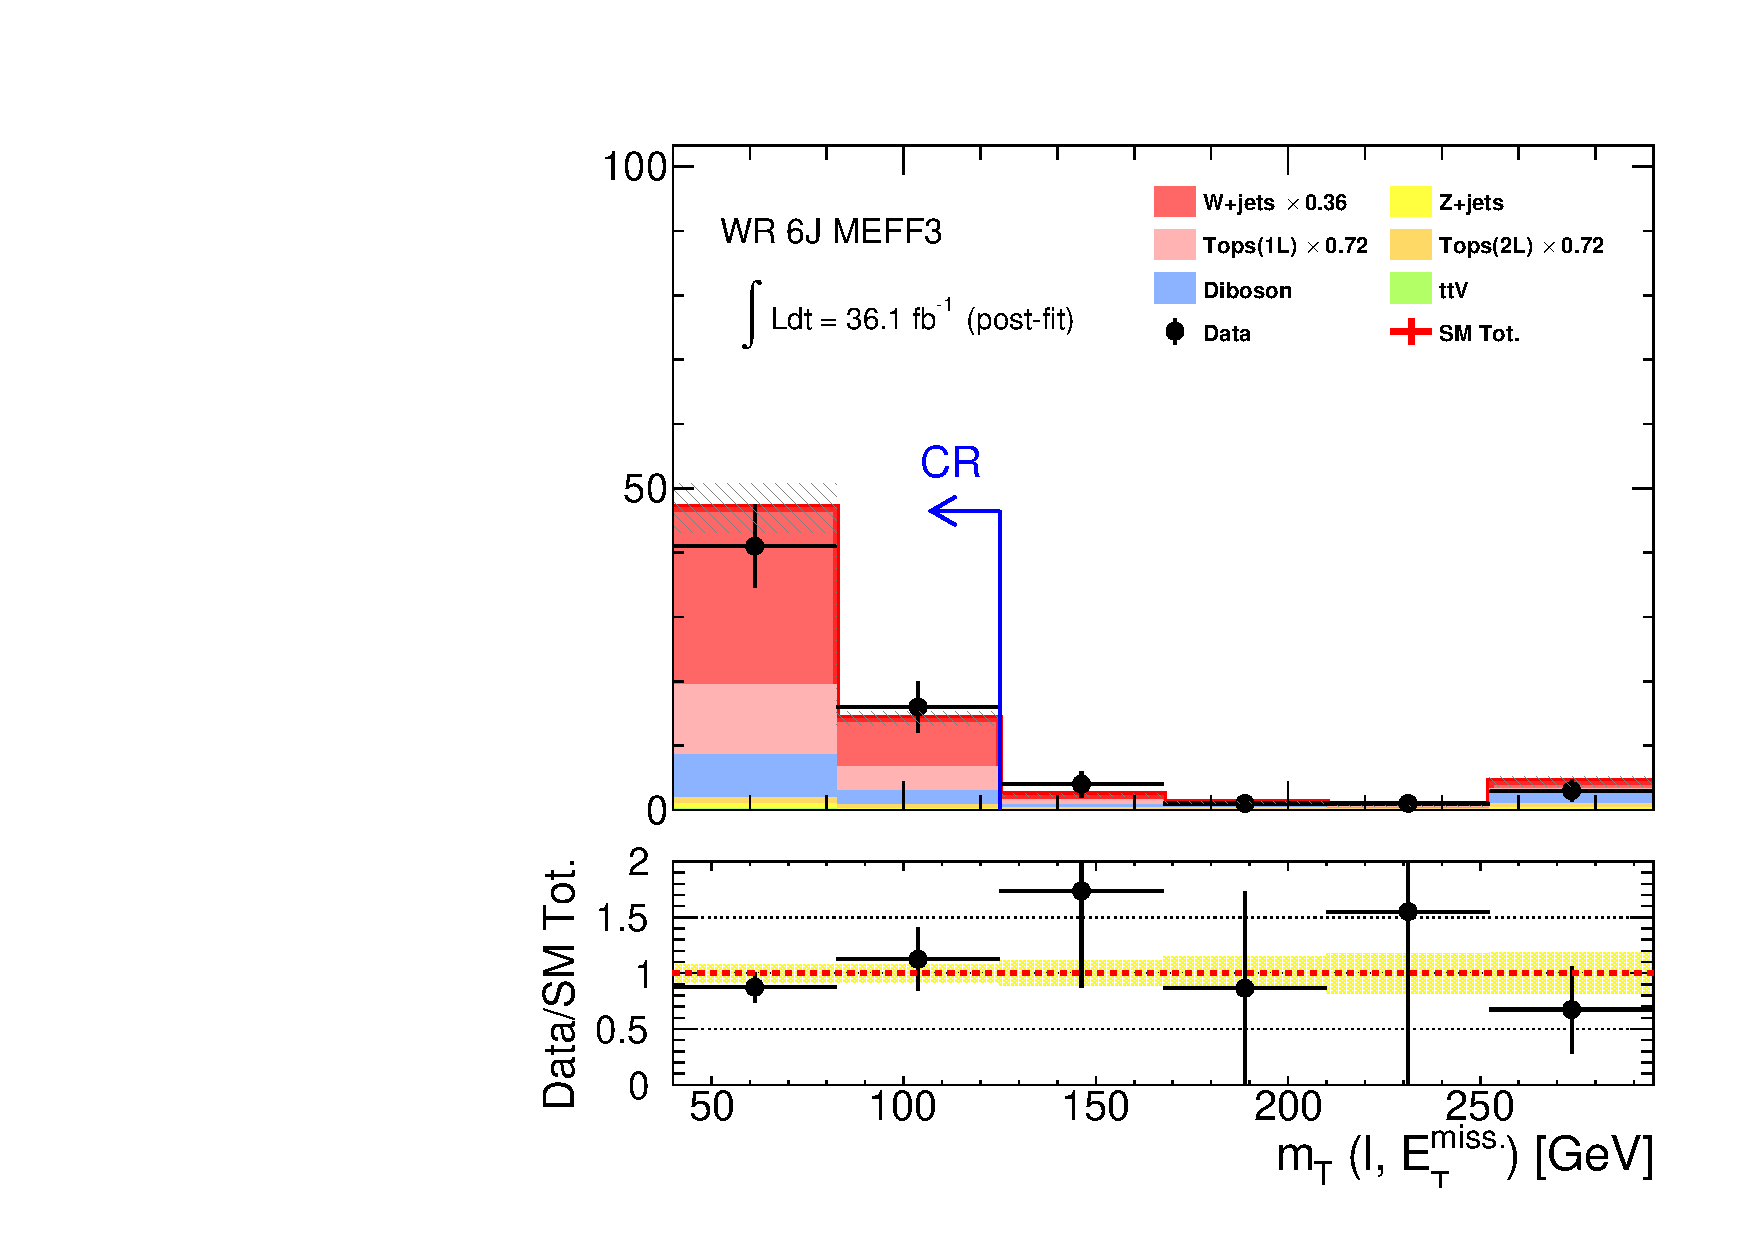
\includegraphics[width=0.41\textwidth]{figures/BGestimation/CRpostFit/WR6JMEFF3/mt__WR6JMEFF3_no_mt_postFit_2SFconfig_noYields.pdf}}
    \subfigure[]{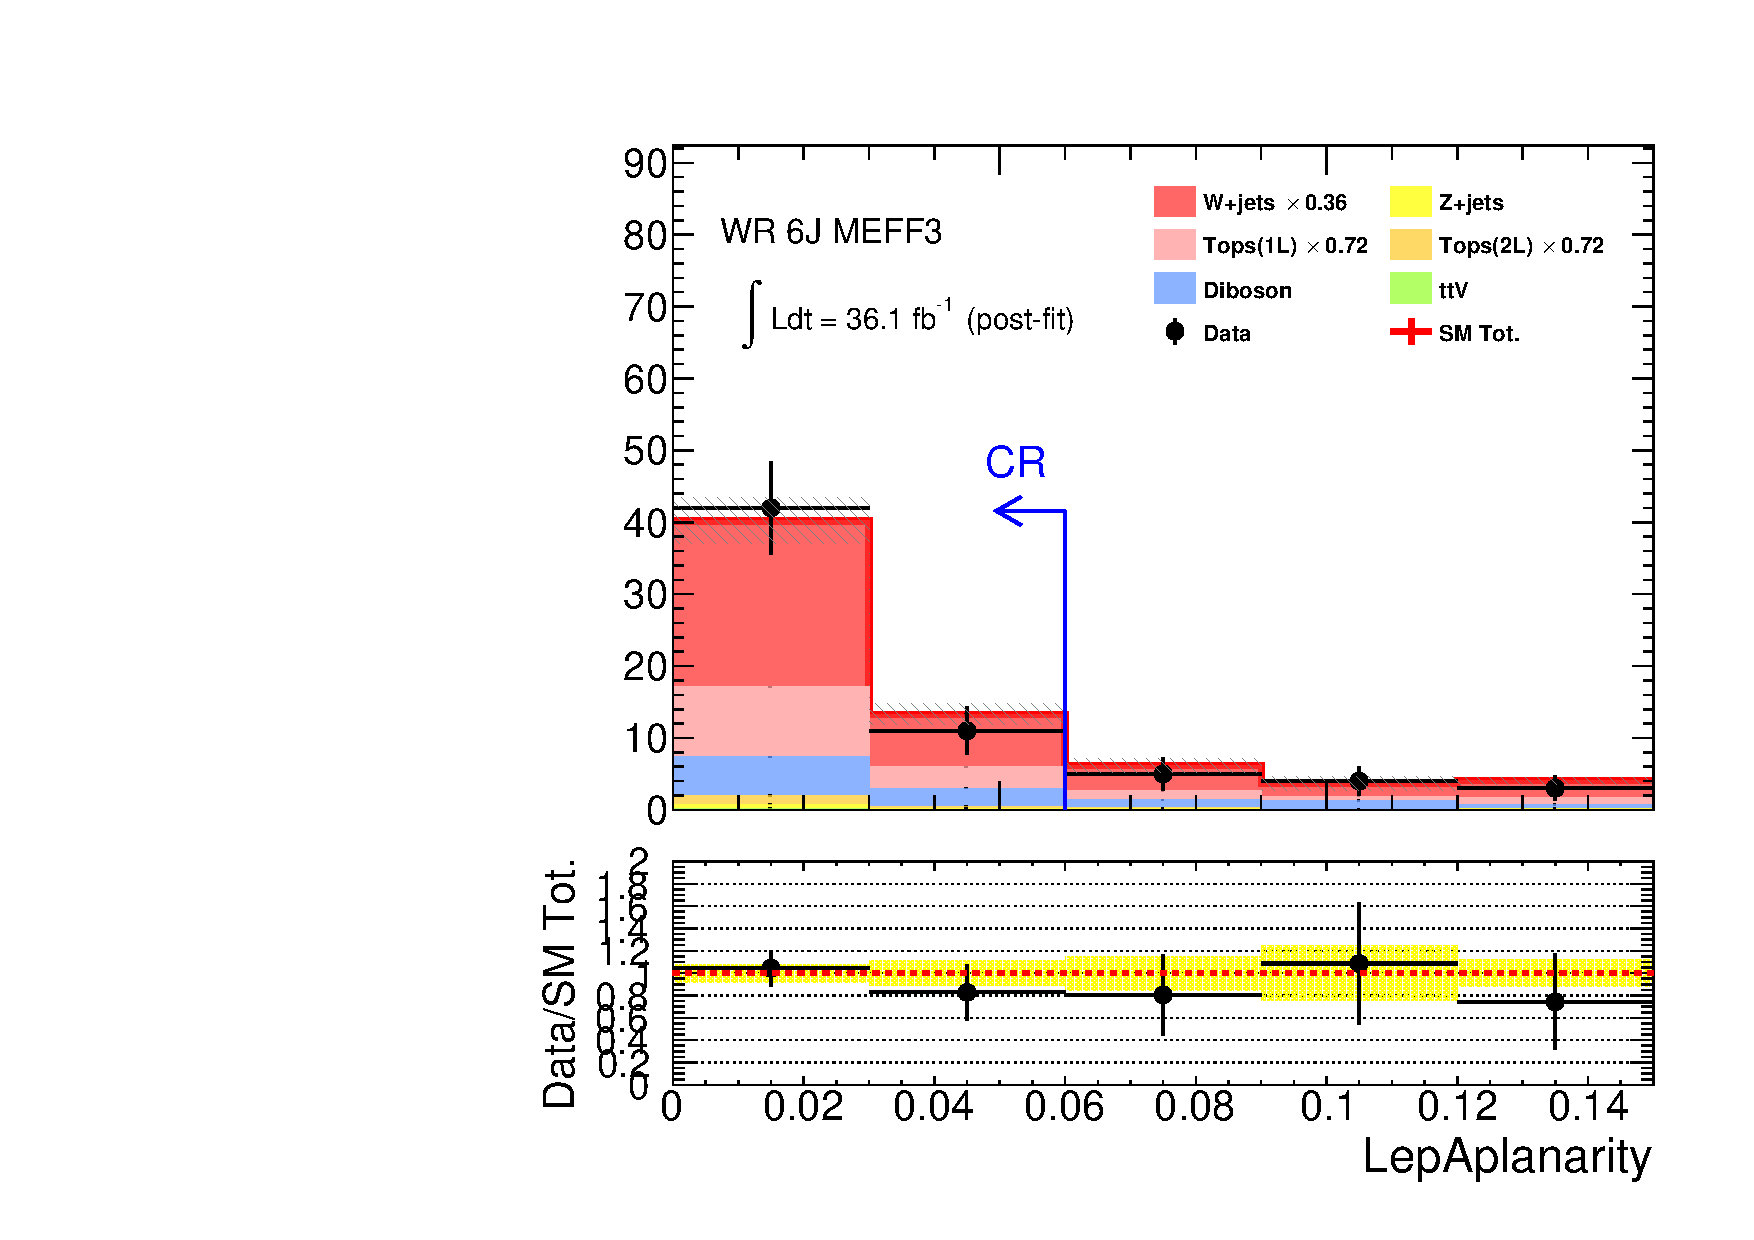
\includegraphics[width=0.41\textwidth]{figures/BGestimation/CRpostFit/WR6JMEFF3/LepAplanarity__WR6JMEFF3_no_LepAplanarity_postFit_2SFconfig_noYields.pdf}}
   \caption{
     Post-fit distruibution of (left) $\mt$ (right) $\apl$.
     (a,b) WR 6J-$\meffIncFirst$.
     (c,d) WR 6J-$\meffIncSecond$.
     (e,f) WR 6J-$\meffIncThird$.
     The yellow band in the bottom panel represents only statistical error. The overflow is included in the highest bin.  
   \label{fig::BGestimation::CRpostFit::WR6J}}    
\end{figure}
%----------------------------------
\clearpage
\begin{figure}[h]
  \centering
    \subfigure[]{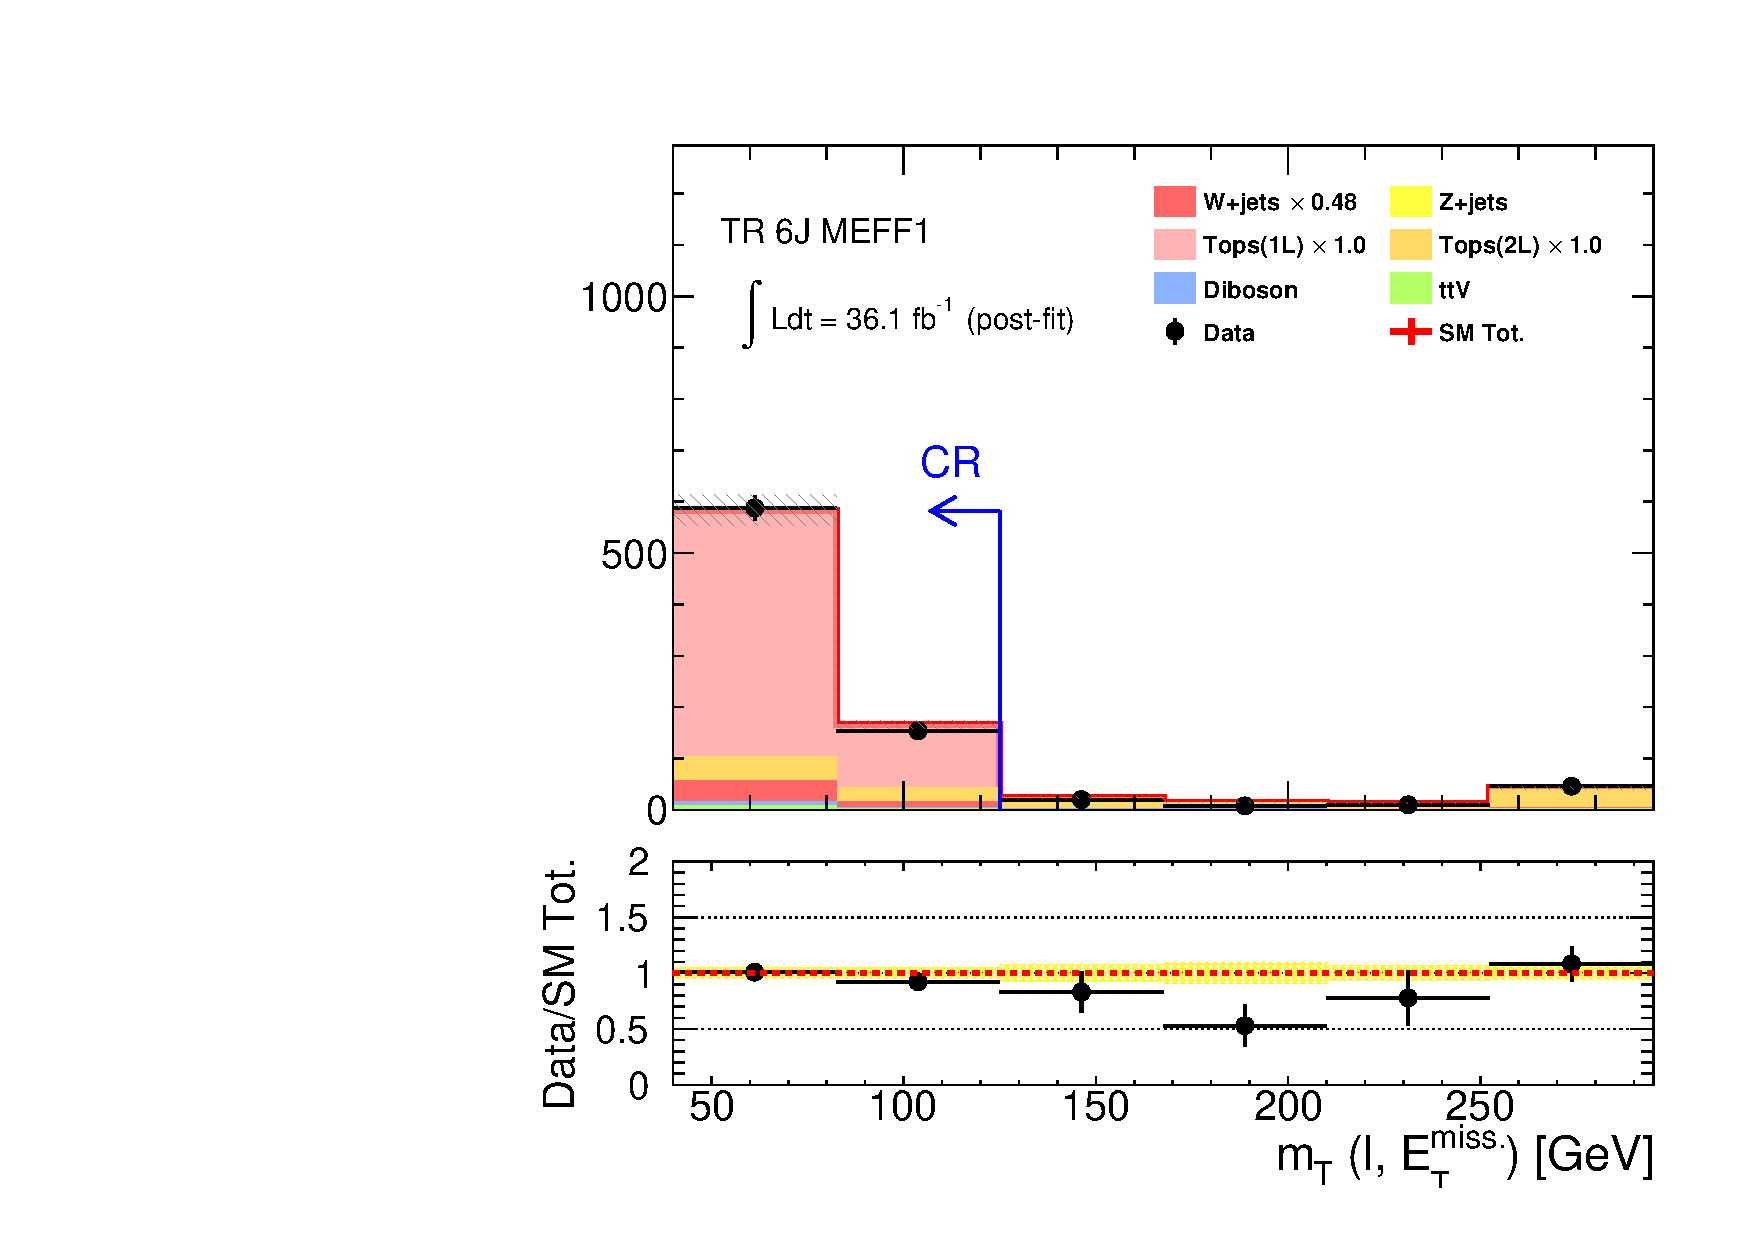
\includegraphics[width=0.41\textwidth]{figures/BGestimation/CRpostFit/TR6JMEFF1/mt__TR6JMEFF1_no_mt_postFit_2SFconfig_noYields.pdf}}
    \subfigure[]{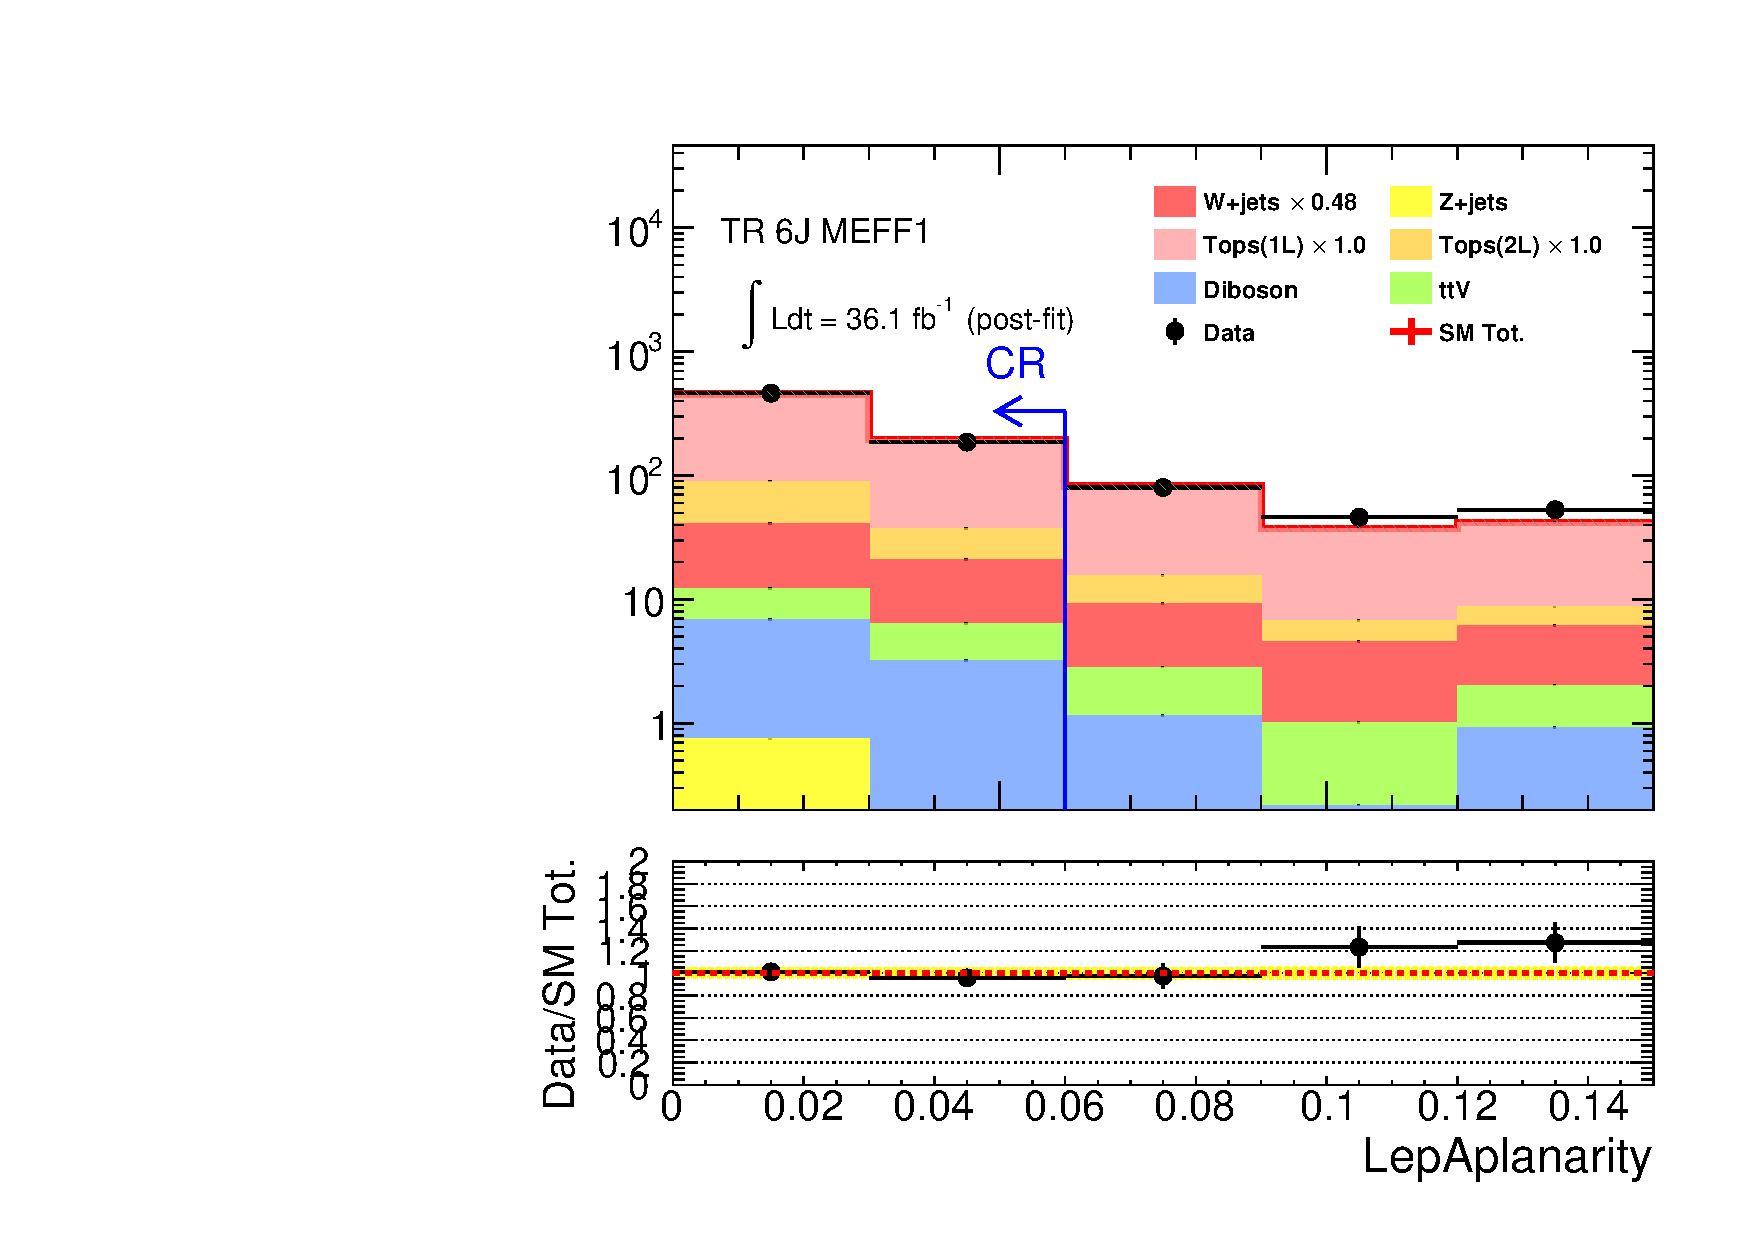
\includegraphics[width=0.41\textwidth]{figures/BGestimation/CRpostFit/TR6JMEFF1/LepAplanarity__TR6JMEFF1_no_LepAplanarity_postFit_2SFconfig_noYields.pdf}}
    \subfigure[]{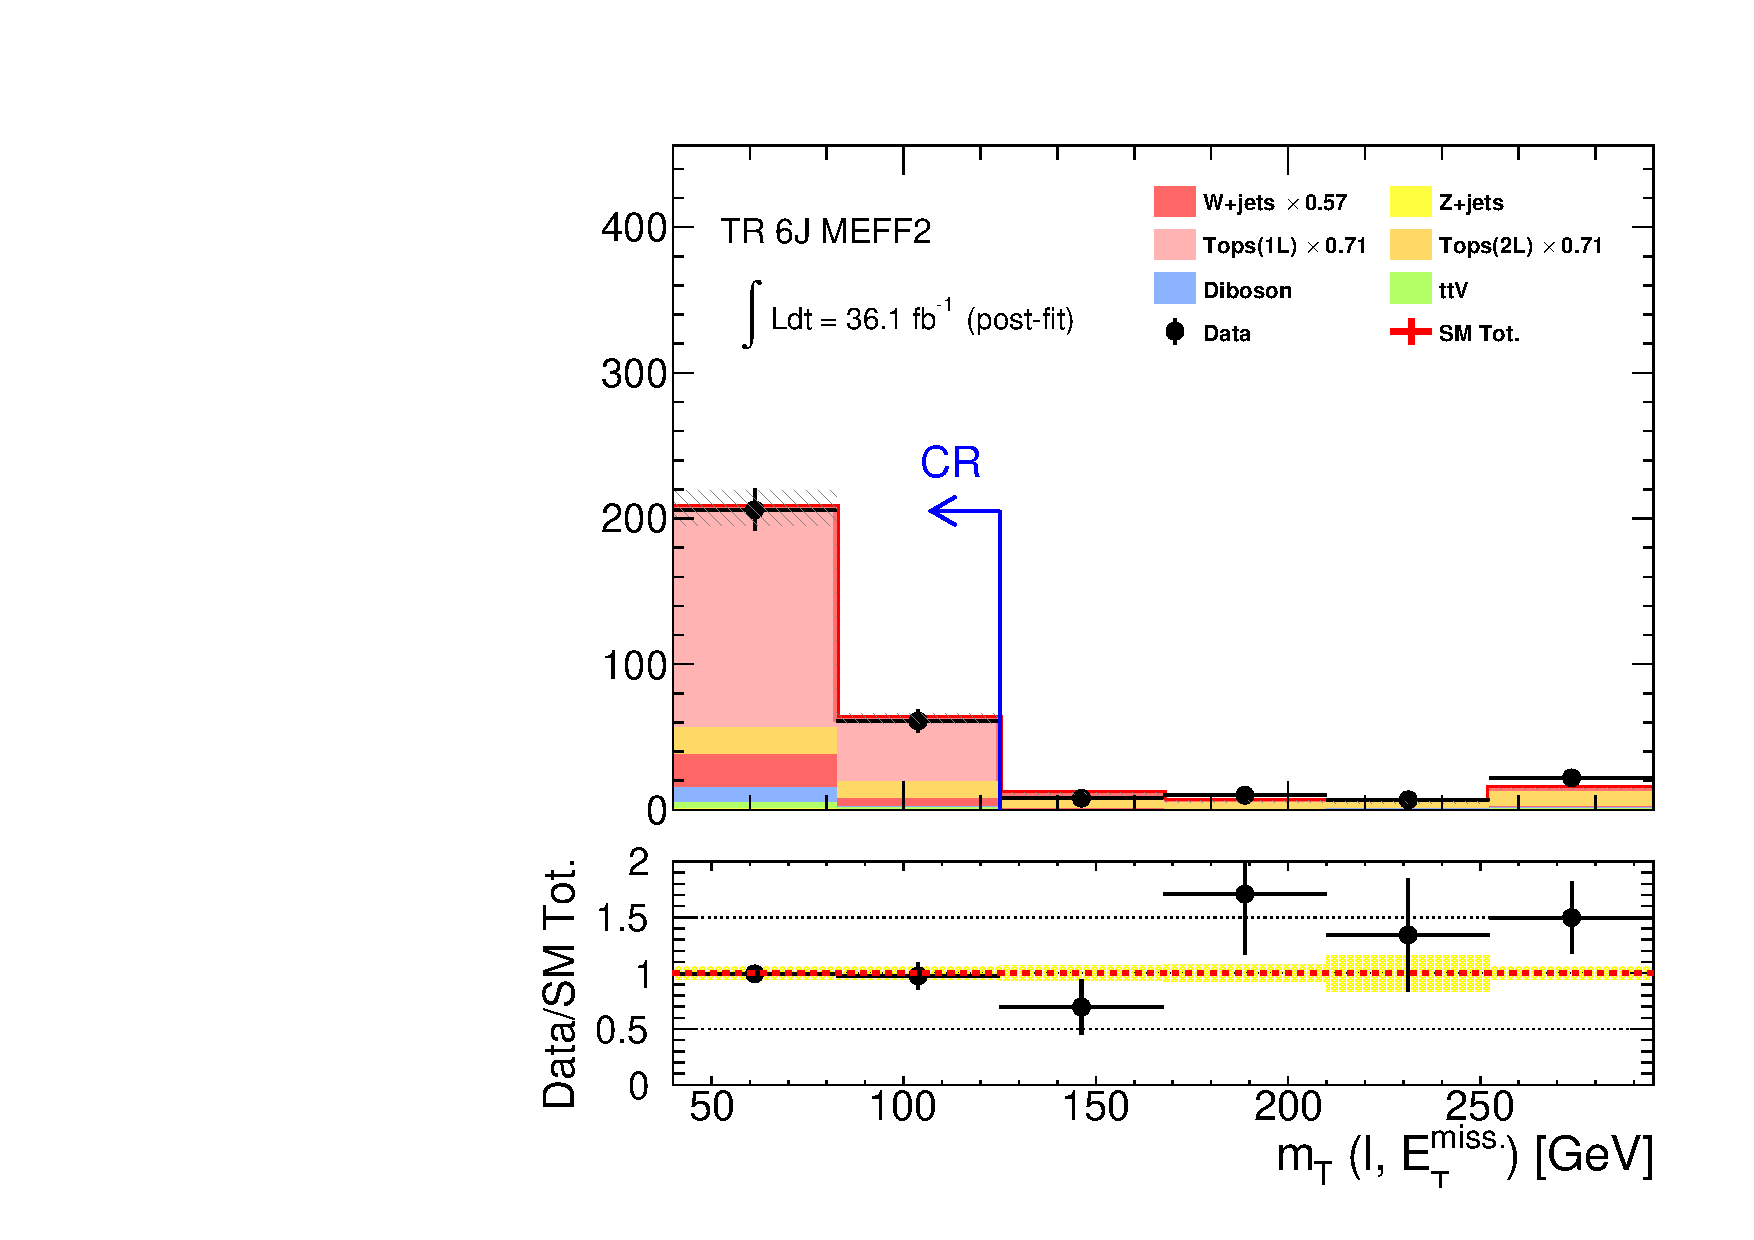
\includegraphics[width=0.41\textwidth]{figures/BGestimation/CRpostFit/TR6JMEFF2/mt__TR6JMEFF2_no_mt_postFit_2SFconfig_noYields.pdf}}
    \subfigure[]{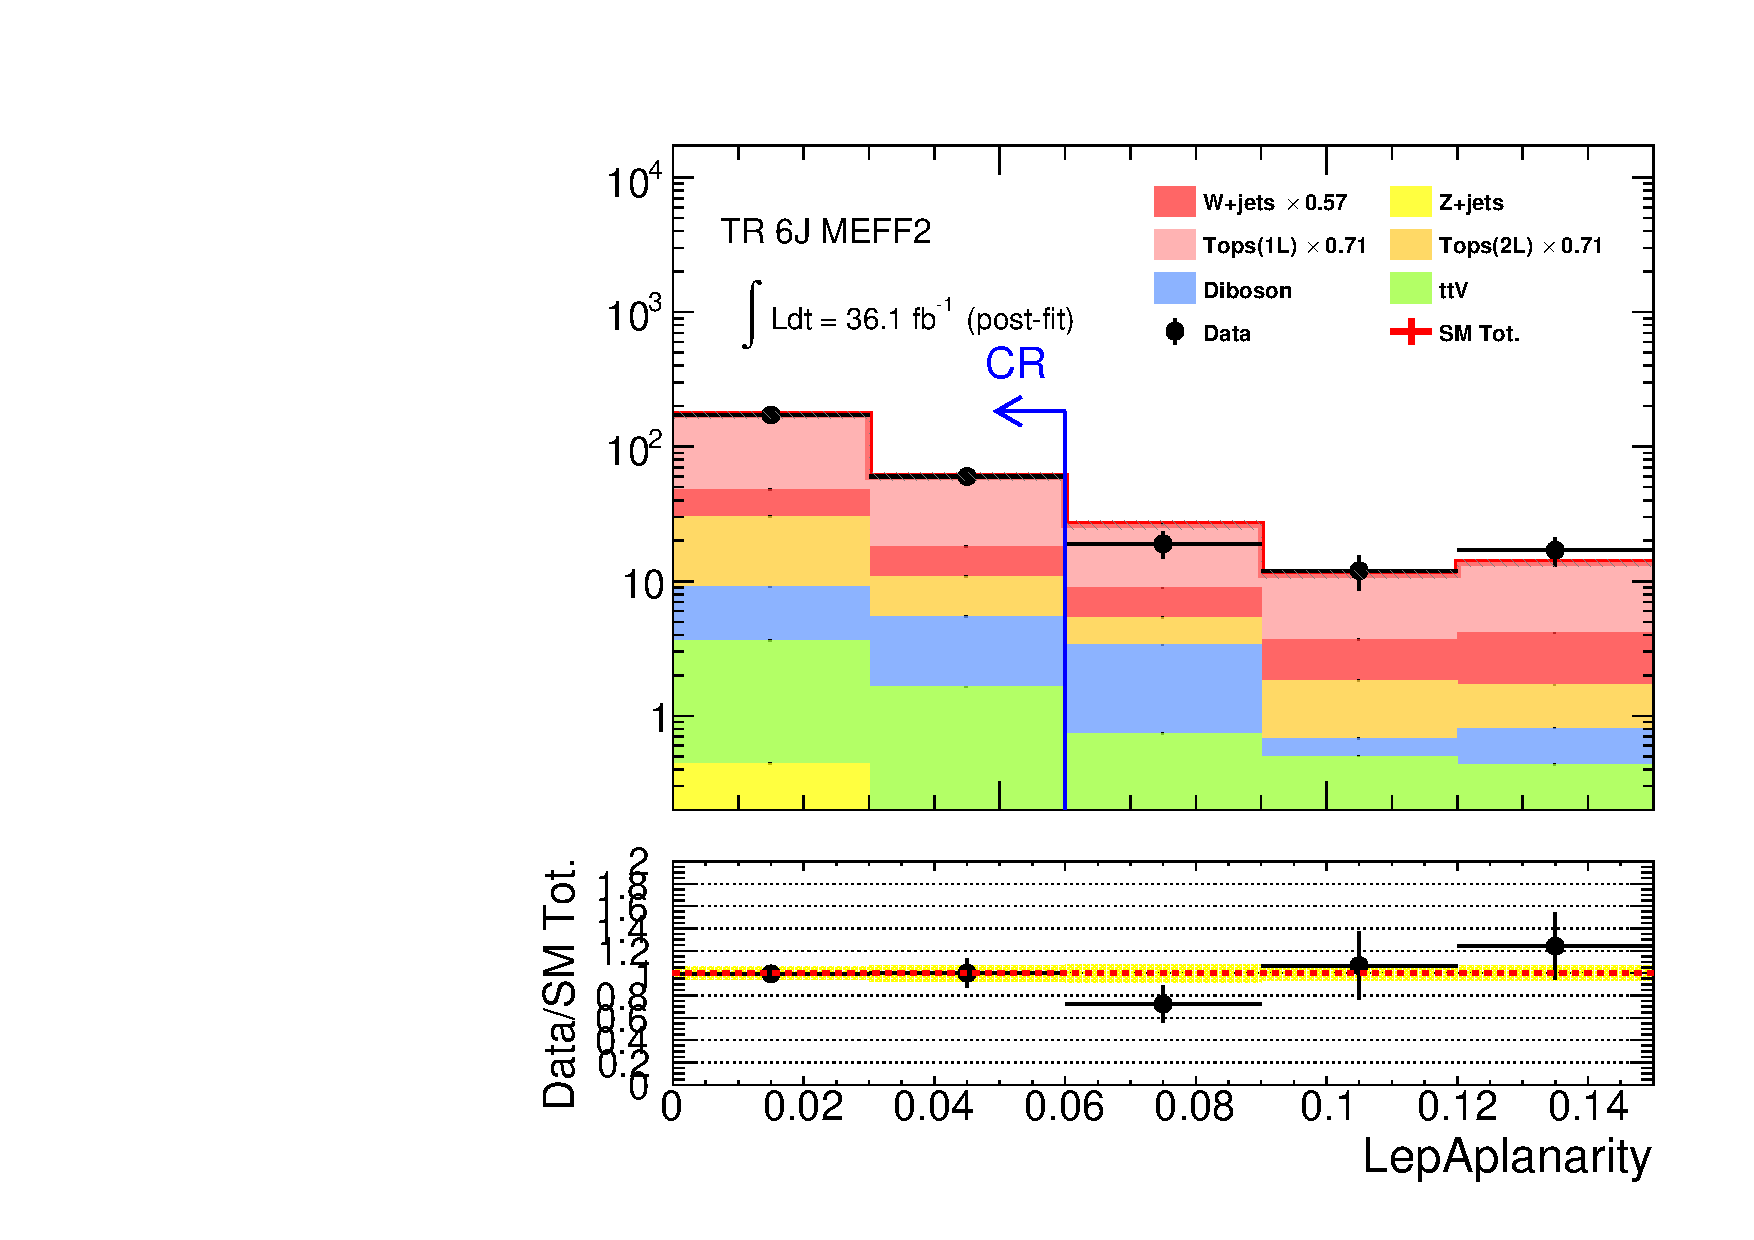
\includegraphics[width=0.41\textwidth]{figures/BGestimation/CRpostFit/TR6JMEFF2/LepAplanarity__TR6JMEFF2_no_LepAplanarity_postFit_2SFconfig_noYields.pdf}}
    \subfigure[]{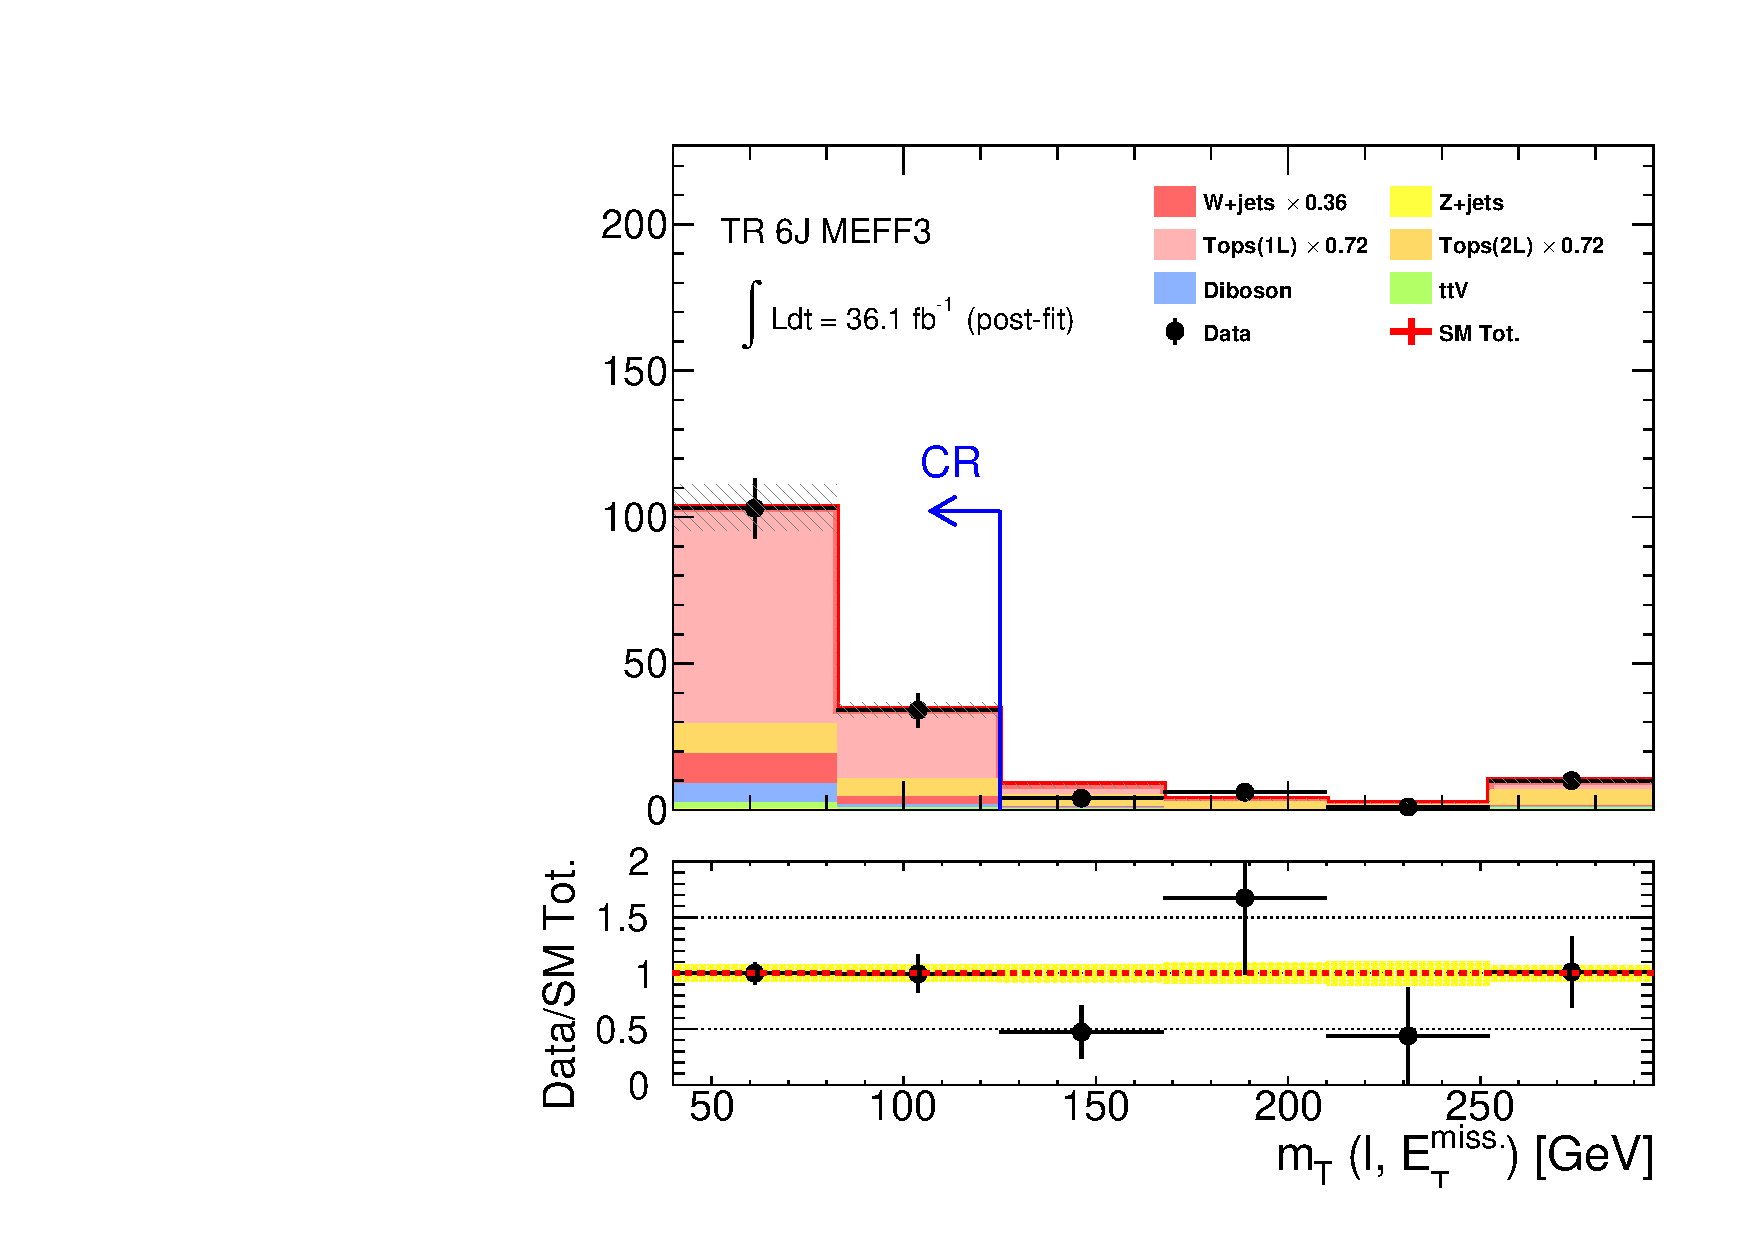
\includegraphics[width=0.41\textwidth]{figures/BGestimation/CRpostFit/TR6JMEFF3/mt__TR6JMEFF3_no_mt_postFit_2SFconfig_noYields.pdf}}
    \subfigure[]{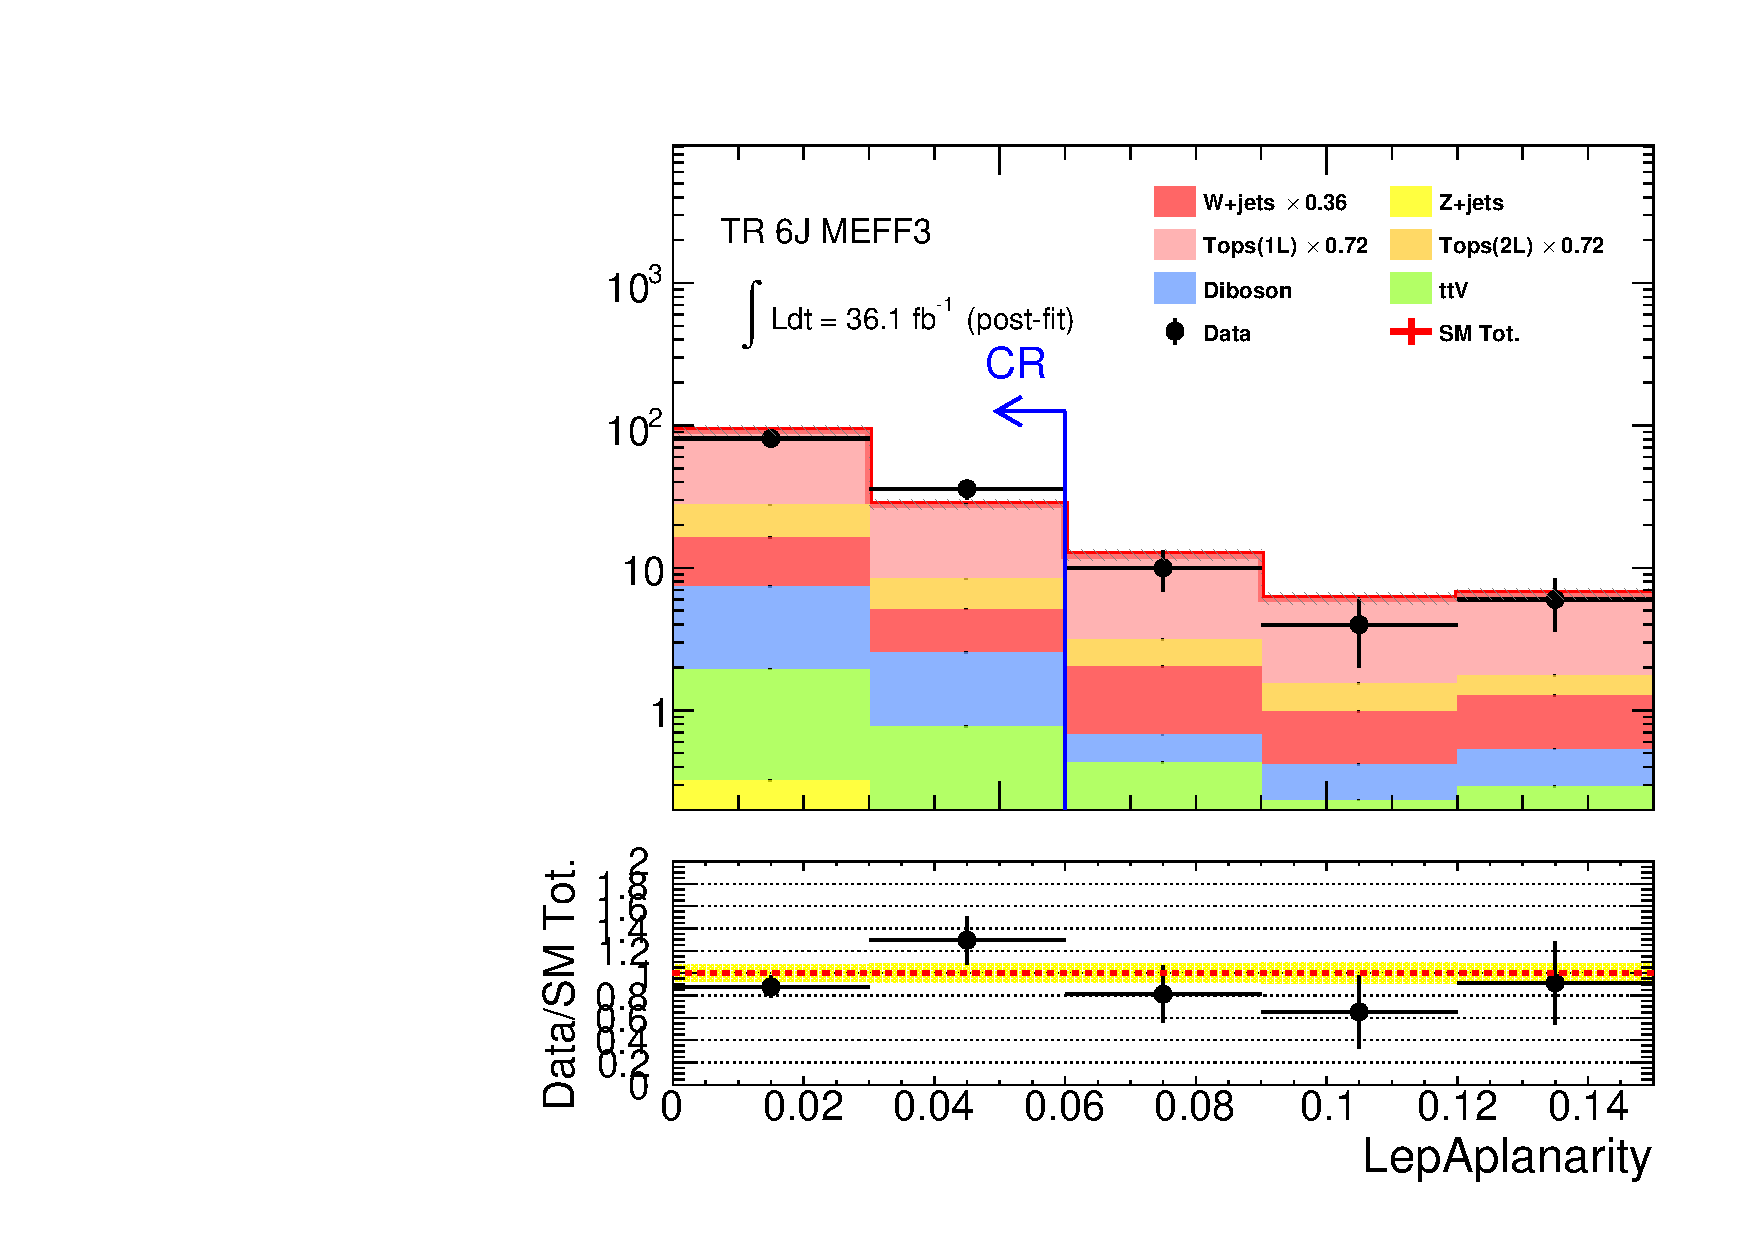
\includegraphics[width=0.41\textwidth]{figures/BGestimation/CRpostFit/TR6JMEFF3/LepAplanarity__TR6JMEFF3_no_LepAplanarity_postFit_2SFconfig_noYields.pdf}}
   \caption{
     Post-fit distruibution of (left) $\mt$ (right) $\apl$.
     (a,b) TR 6J-$\meffIncFirst$.
     (c,d) TR 6J-$\meffIncSecond$.
     (e,f) TR 6J-$\meffIncThird$.
     The yellow band in the bottom panel represents only statistical error. The overflow is included in the highest bin.  
   \label{fig::BGestimation::CRpostFit::TR6J}}    
\end{figure}
%----------------------------------



\clearpage
% -------------- varx ---------
\begin{figure}[h]
  \centering
    \subfigure[]{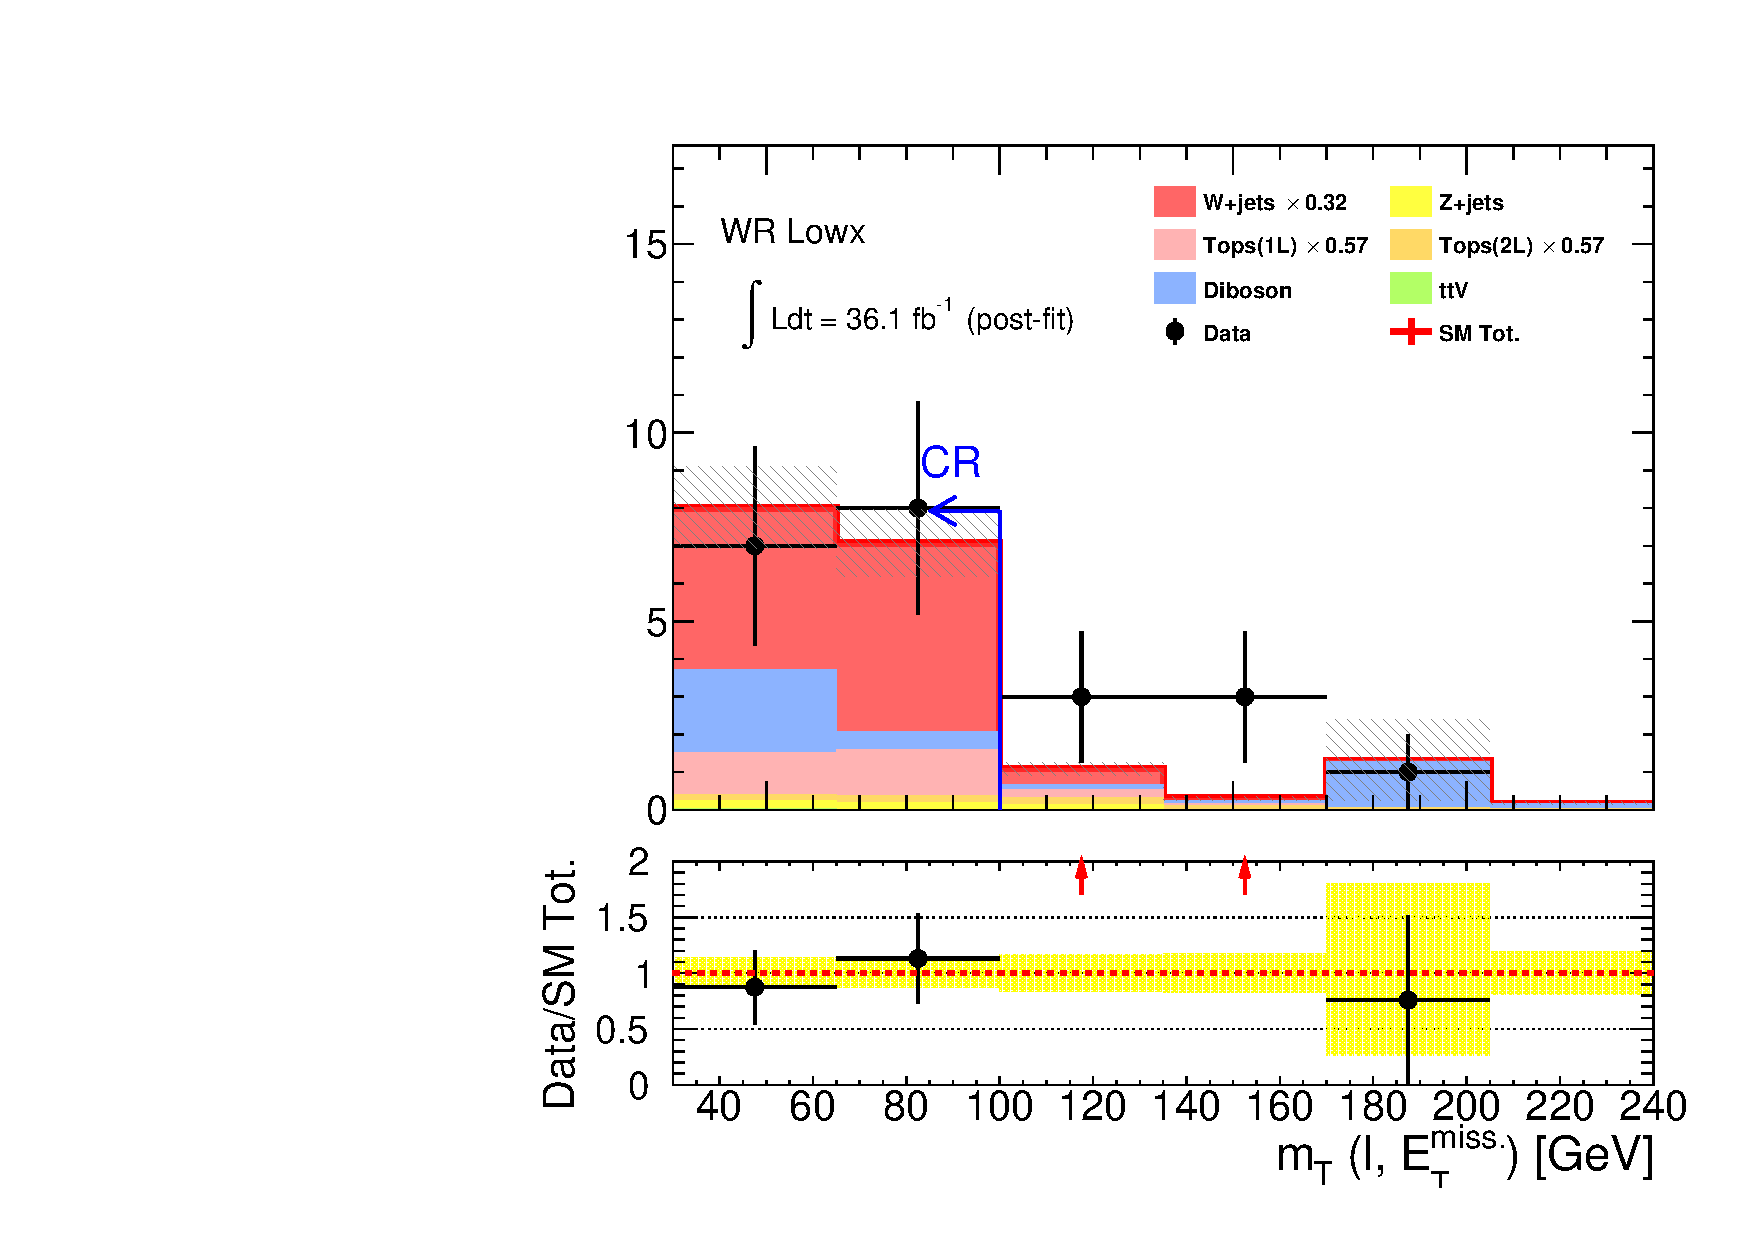
\includegraphics[width=0.41\textwidth]{figures/BGestimation/CRpostFit/WRLowx/mt__WRLowx_no_mt_postFit_2SFconfig_noYields.pdf}}
    \subfigure[]{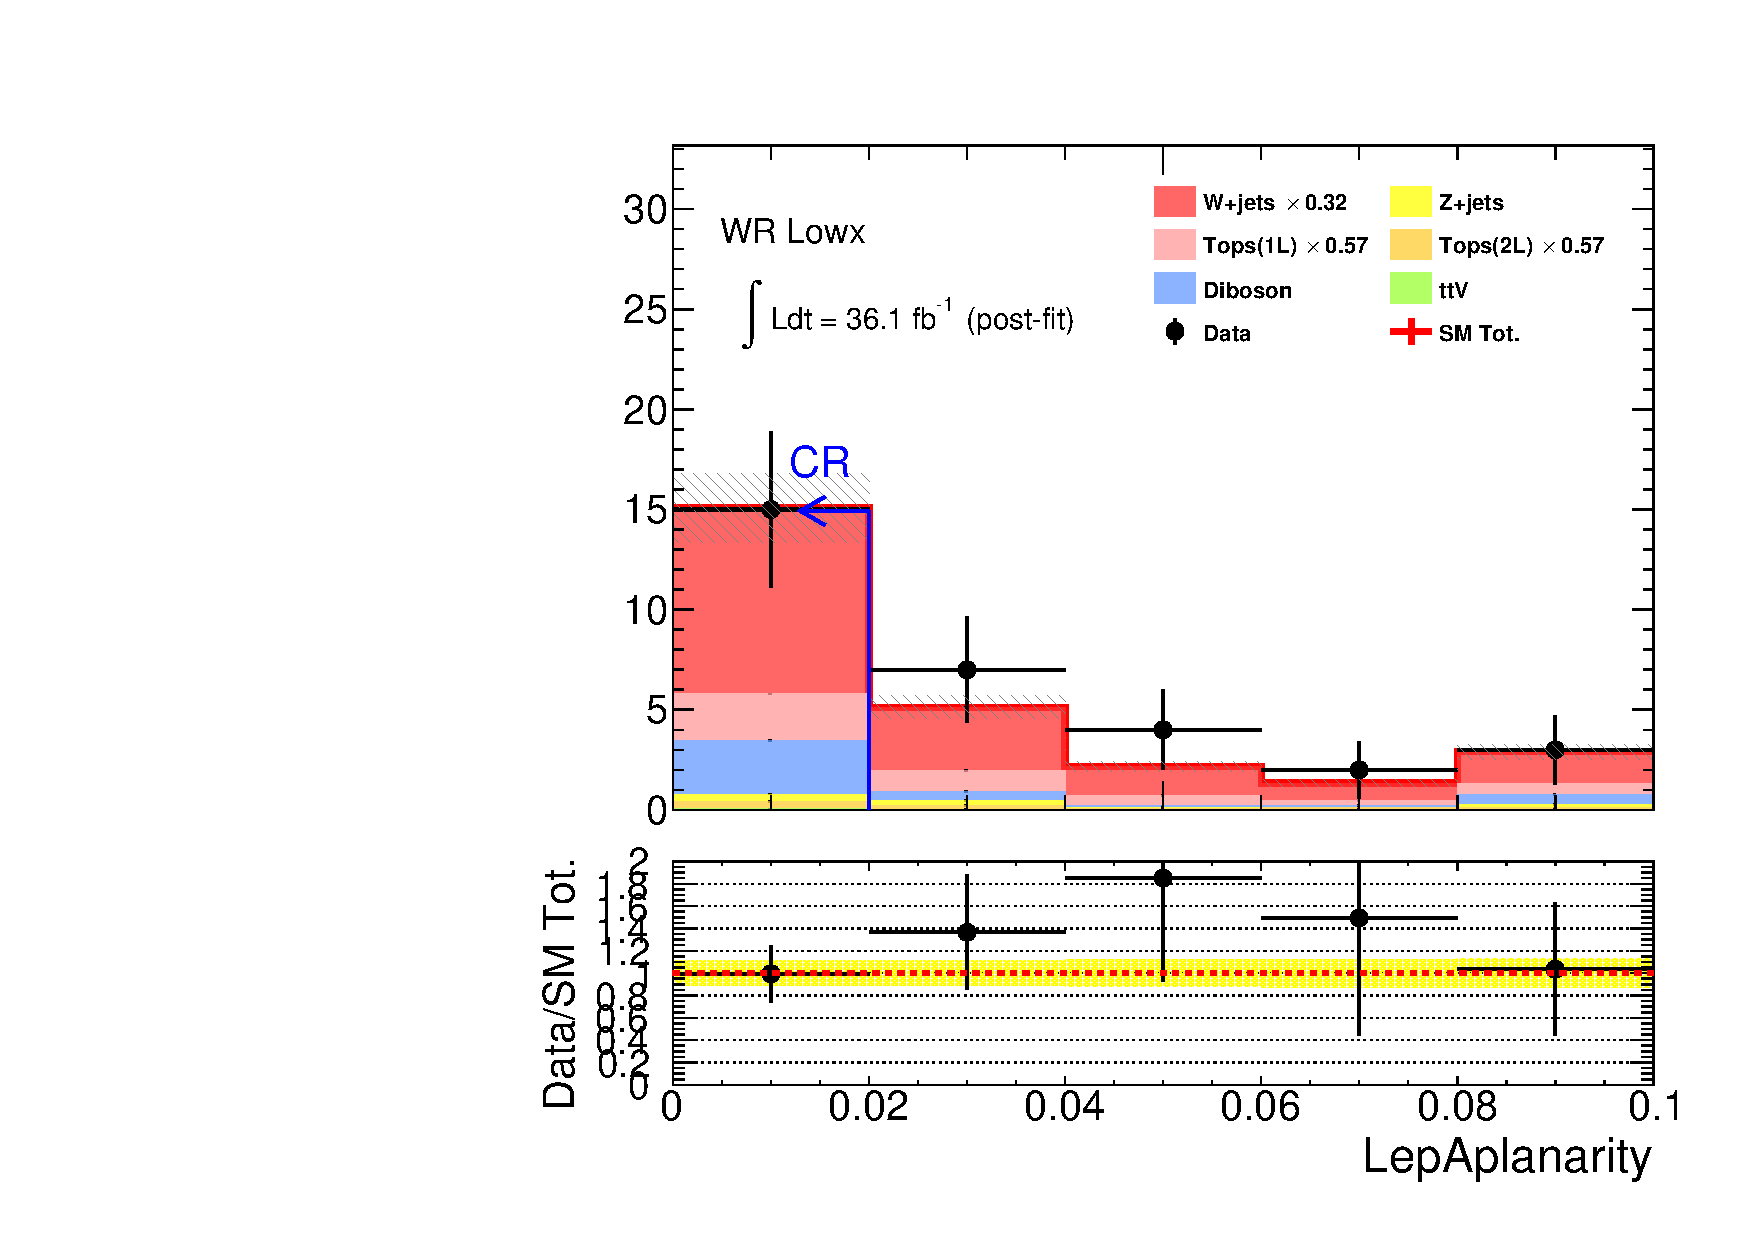
\includegraphics[width=0.41\textwidth]{figures/BGestimation/CRpostFit/WRLowx/LepAplanarity__WRLowx_no_LepAplanarity_postFit_2SFconfig_noYields.pdf}}
    \subfigure[]{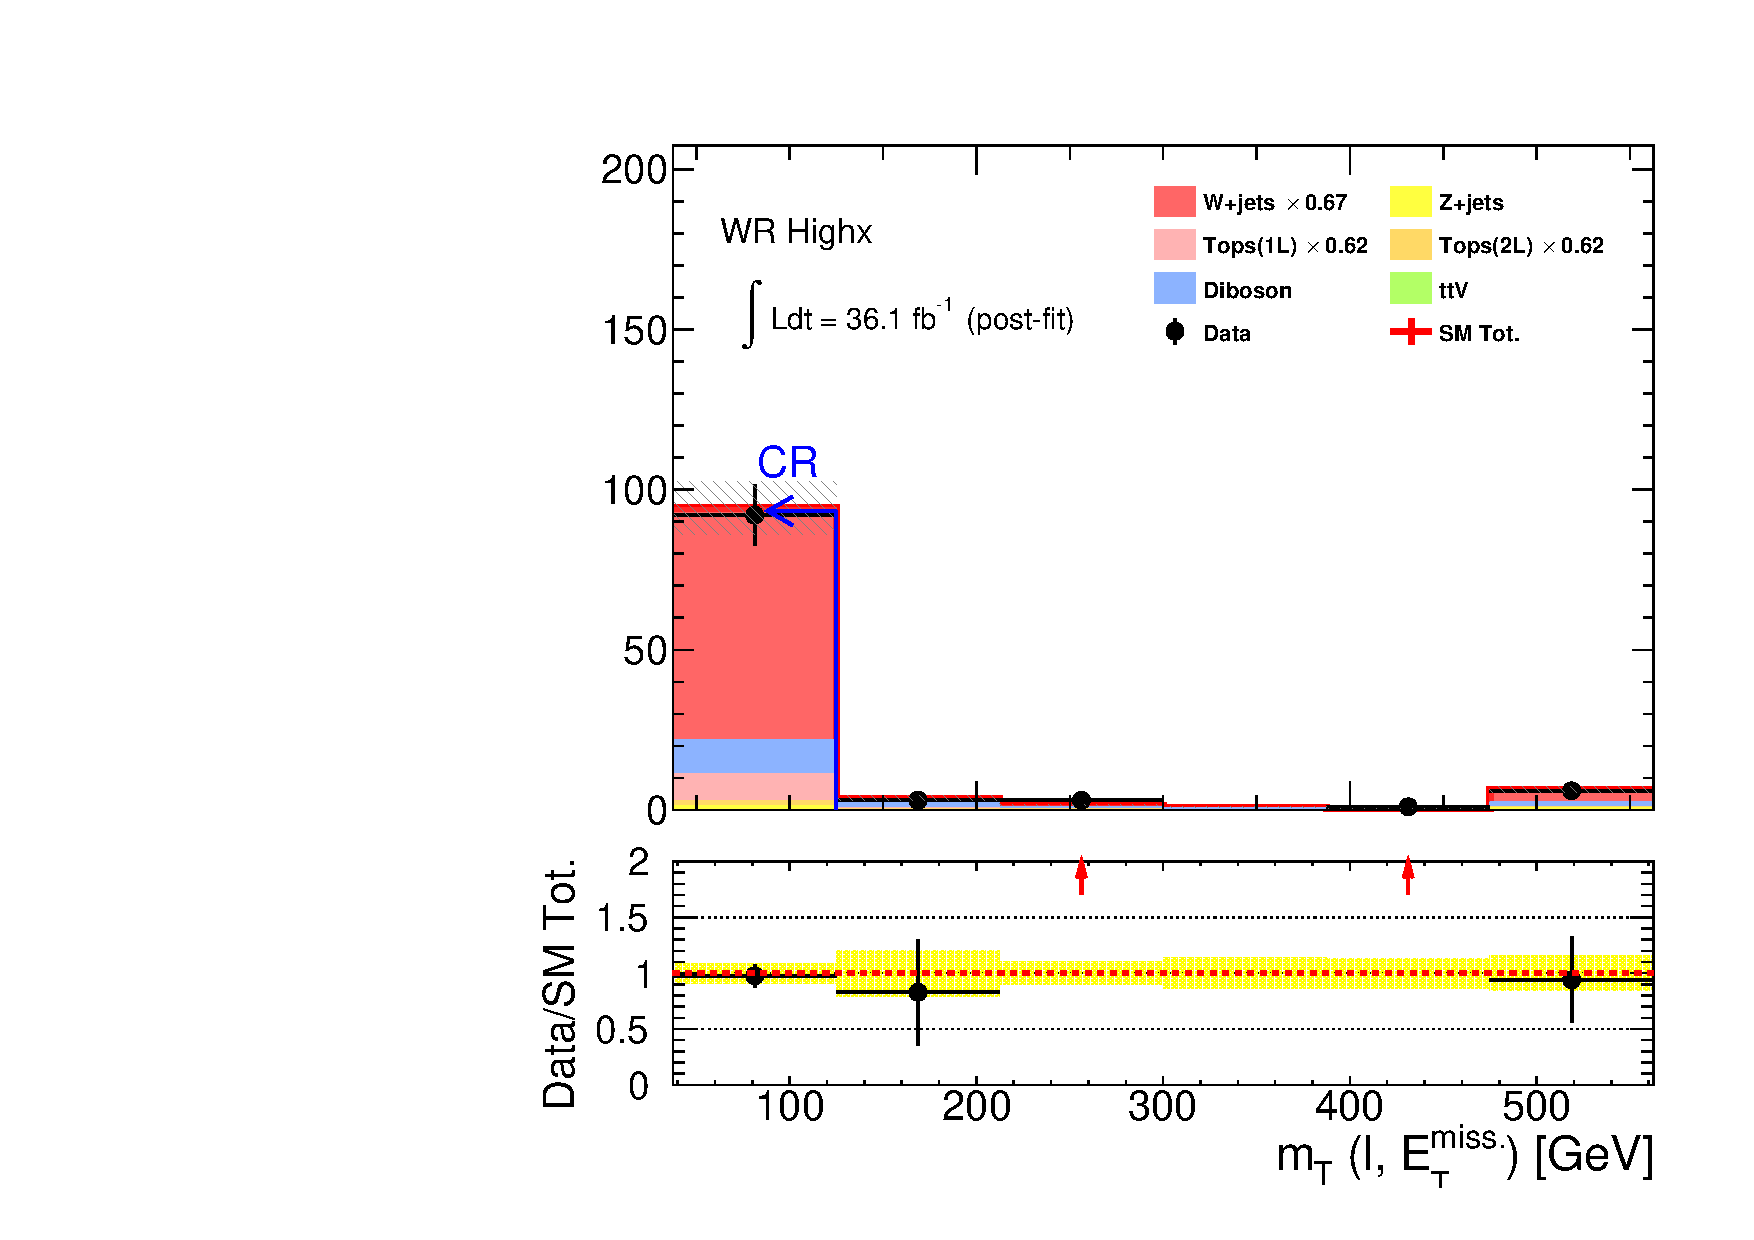
\includegraphics[width=0.41\textwidth]{figures/BGestimation/CRpostFit/WRHighx/mt__WRHighx_no_mt_postFit_2SFconfig_noYields.pdf}}
    \subfigure[]{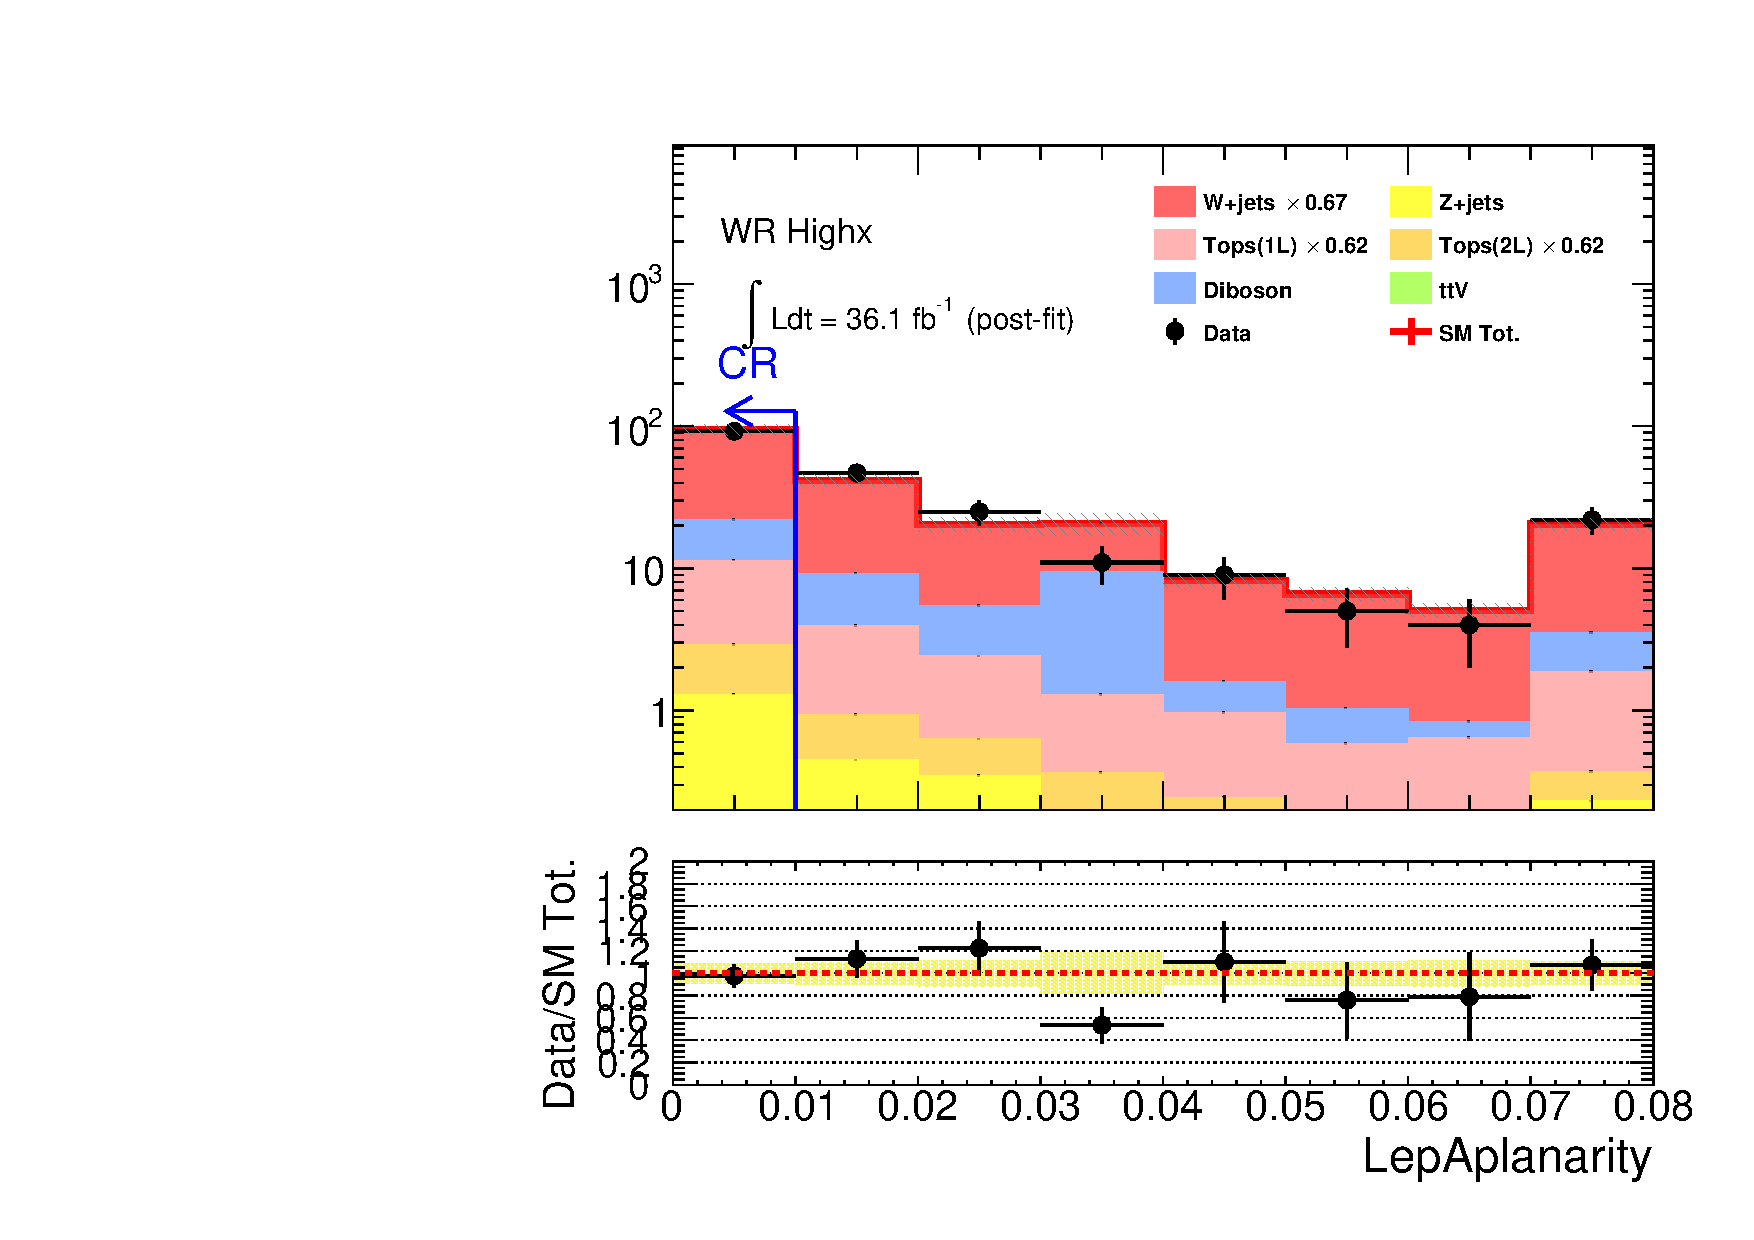
\includegraphics[width=0.41\textwidth]{figures/BGestimation/CRpostFit/WRHighx/LepAplanarity__WRHighx_no_LepAplanarity_postFit_2SFconfig_noYields.pdf}}
   \caption{   
     Post-fit distruibution of (left) $\mt$ (right) $\apl$.
     (a,b) WR Low-x.
     (c,d) WR High-x.
     The yellow band in the bottom panel represents only statistical error. The overflow is included in the highest bin.  
\label{fig::BGestimation::CRpostFit::WRVarx}}    
\end{figure}
%----------------------------------
\clearpage
\begin{figure}[h]
  \centering
    \subfigure[]{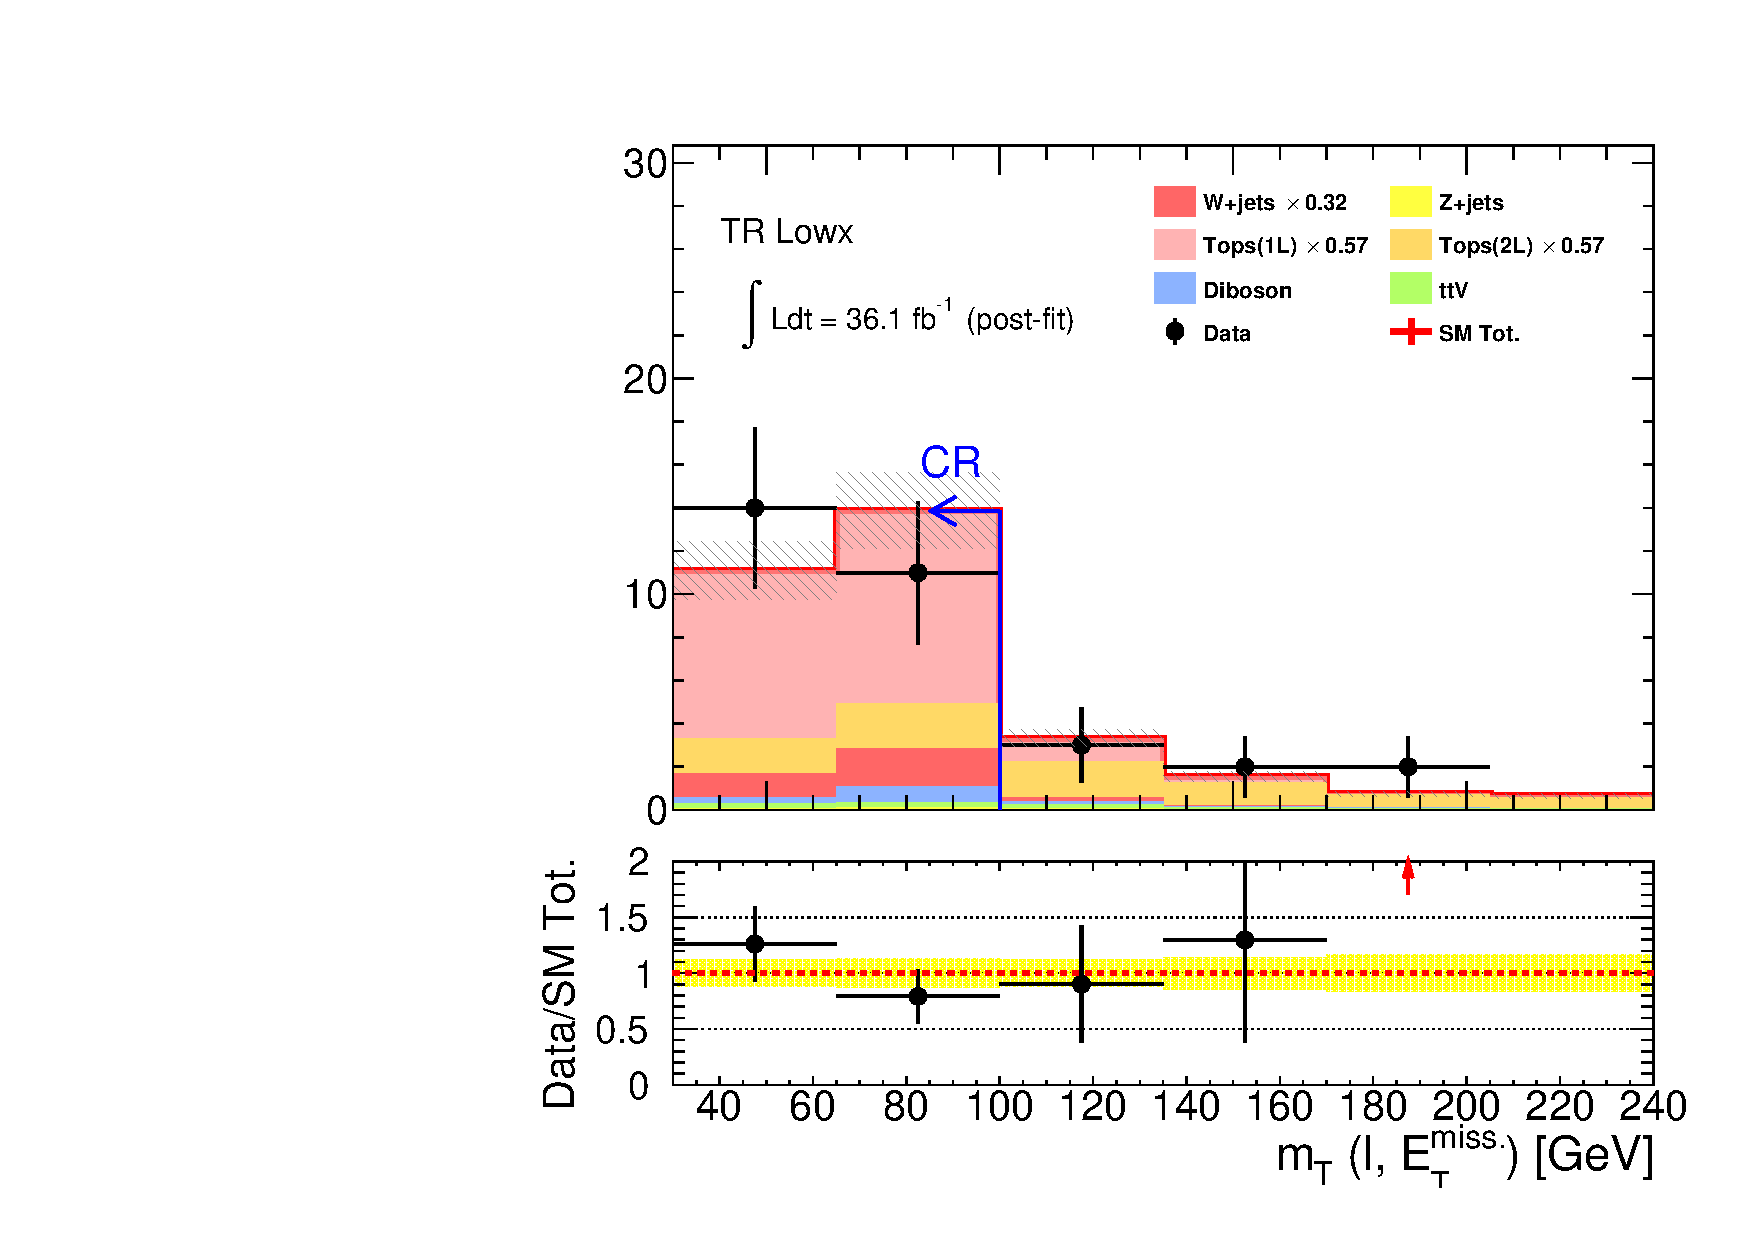
\includegraphics[width=0.41\textwidth]{figures/BGestimation/CRpostFit/TRLowx/mt__TRLowx_no_mt_postFit_2SFconfig_noYields.pdf}}
    \subfigure[]{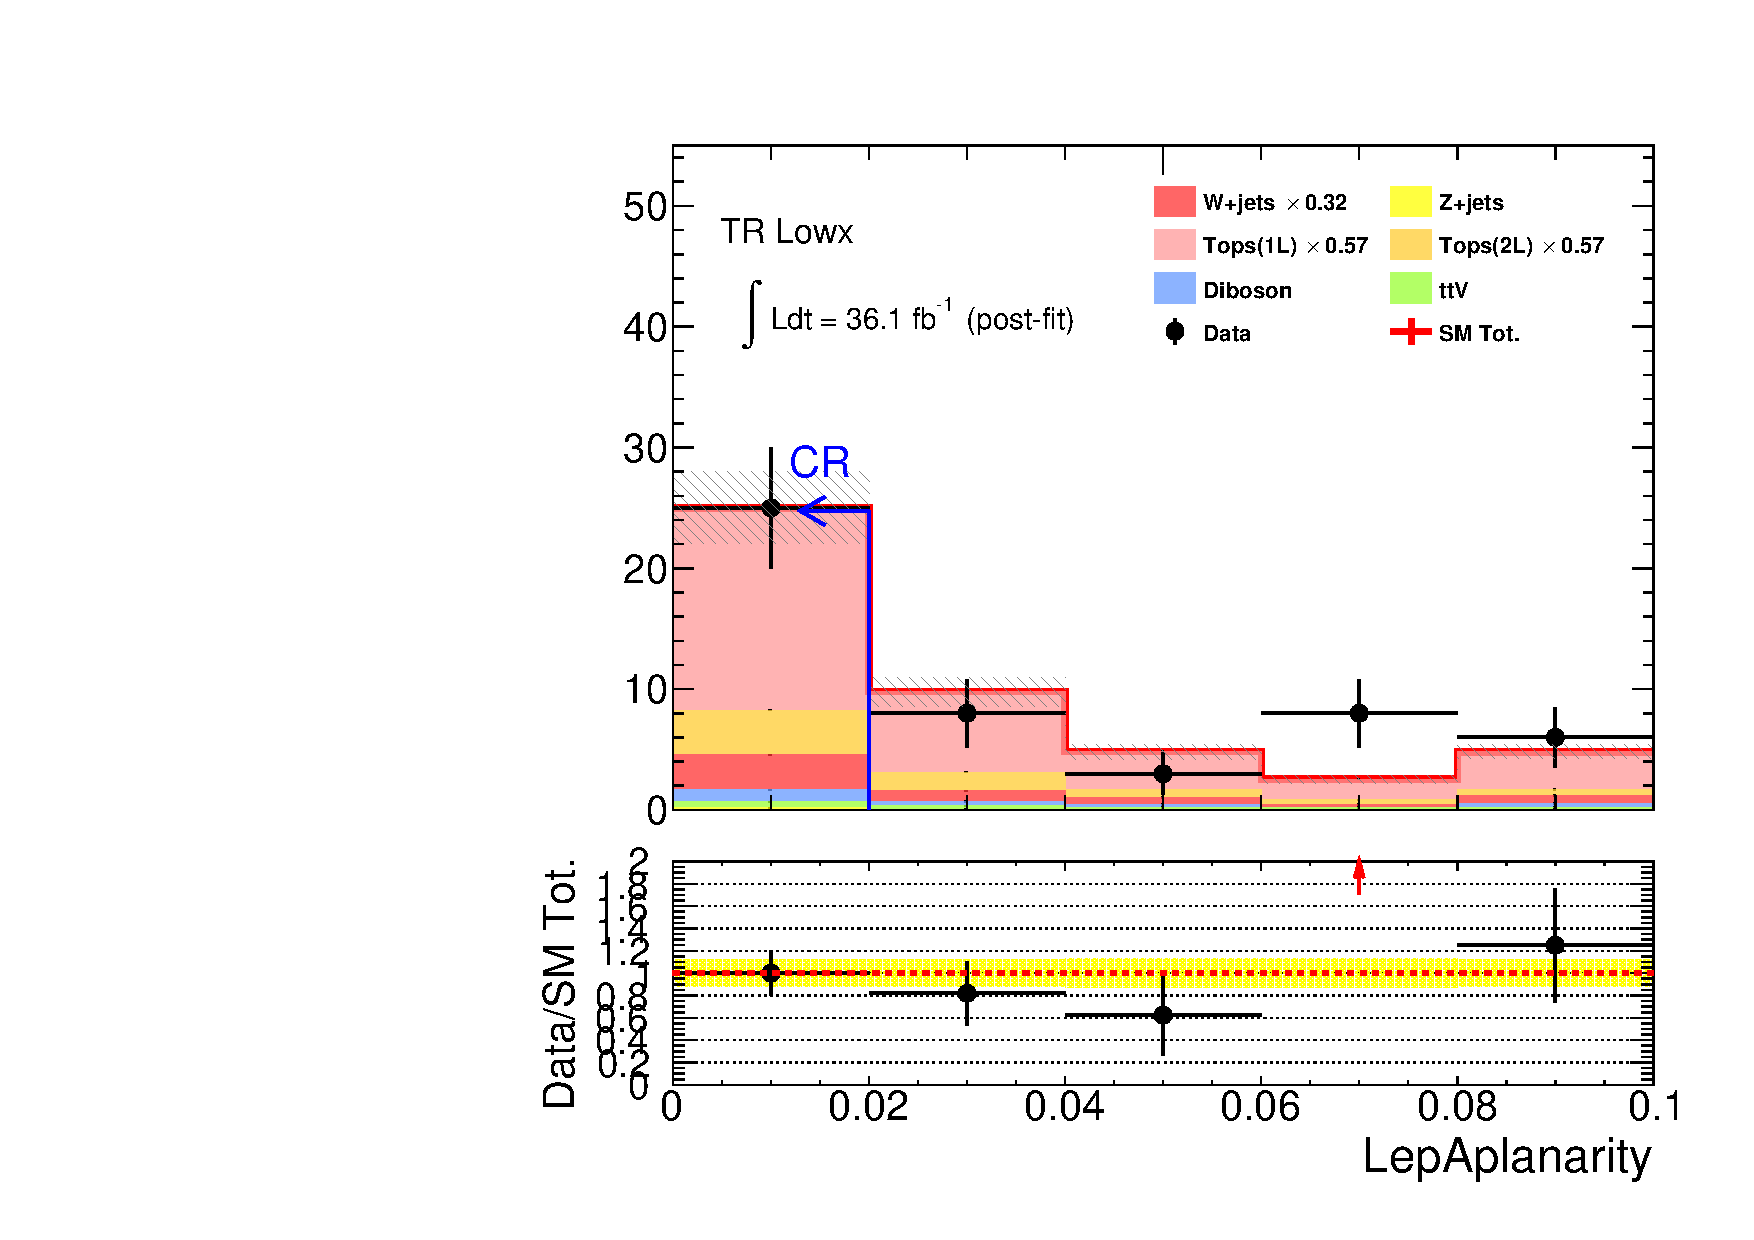
\includegraphics[width=0.41\textwidth]{figures/BGestimation/CRpostFit/TRLowx/LepAplanarity__TRLowx_no_LepAplanarity_postFit_2SFconfig_noYields.pdf}}
    \subfigure[]{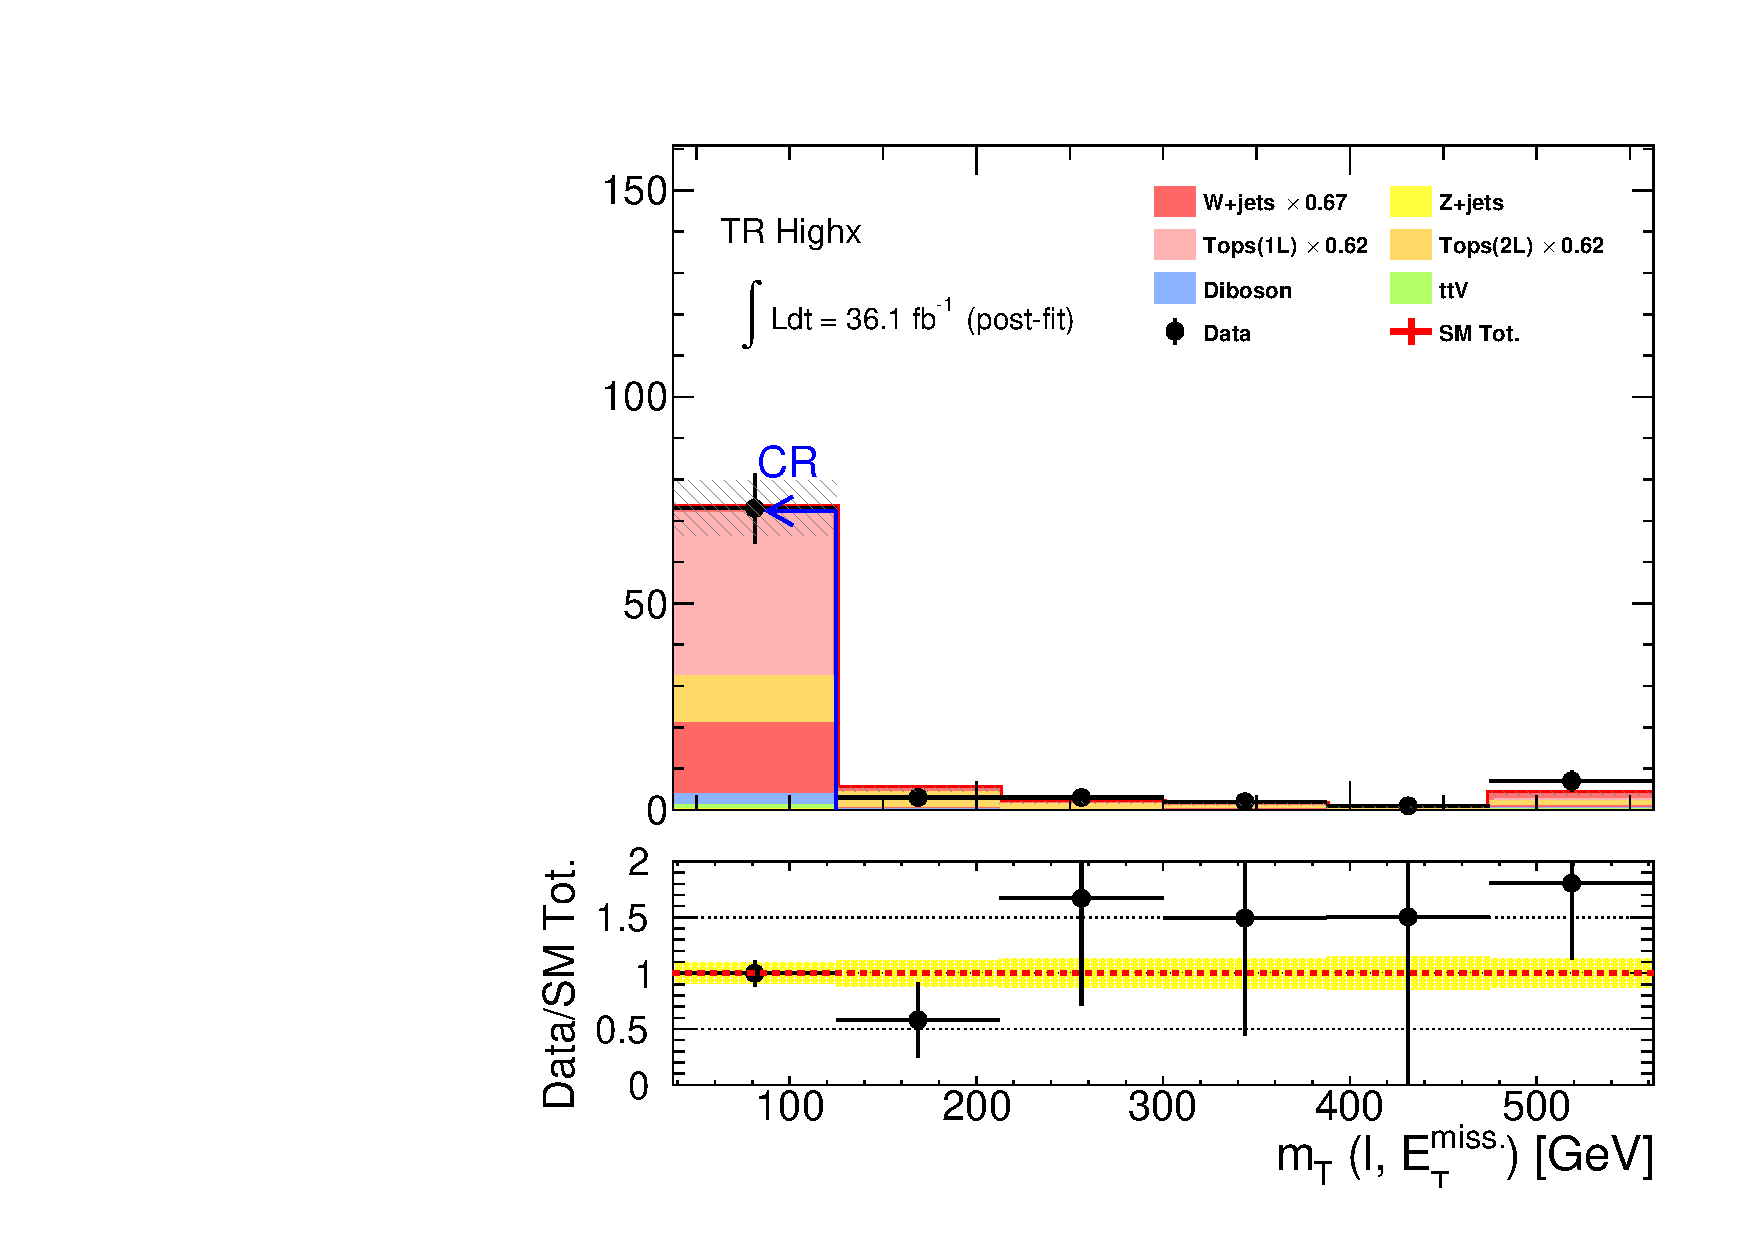
\includegraphics[width=0.41\textwidth]{figures/BGestimation/CRpostFit/TRHighx/mt__TRHighx_no_mt_postFit_2SFconfig_noYields.pdf}}
    \subfigure[]{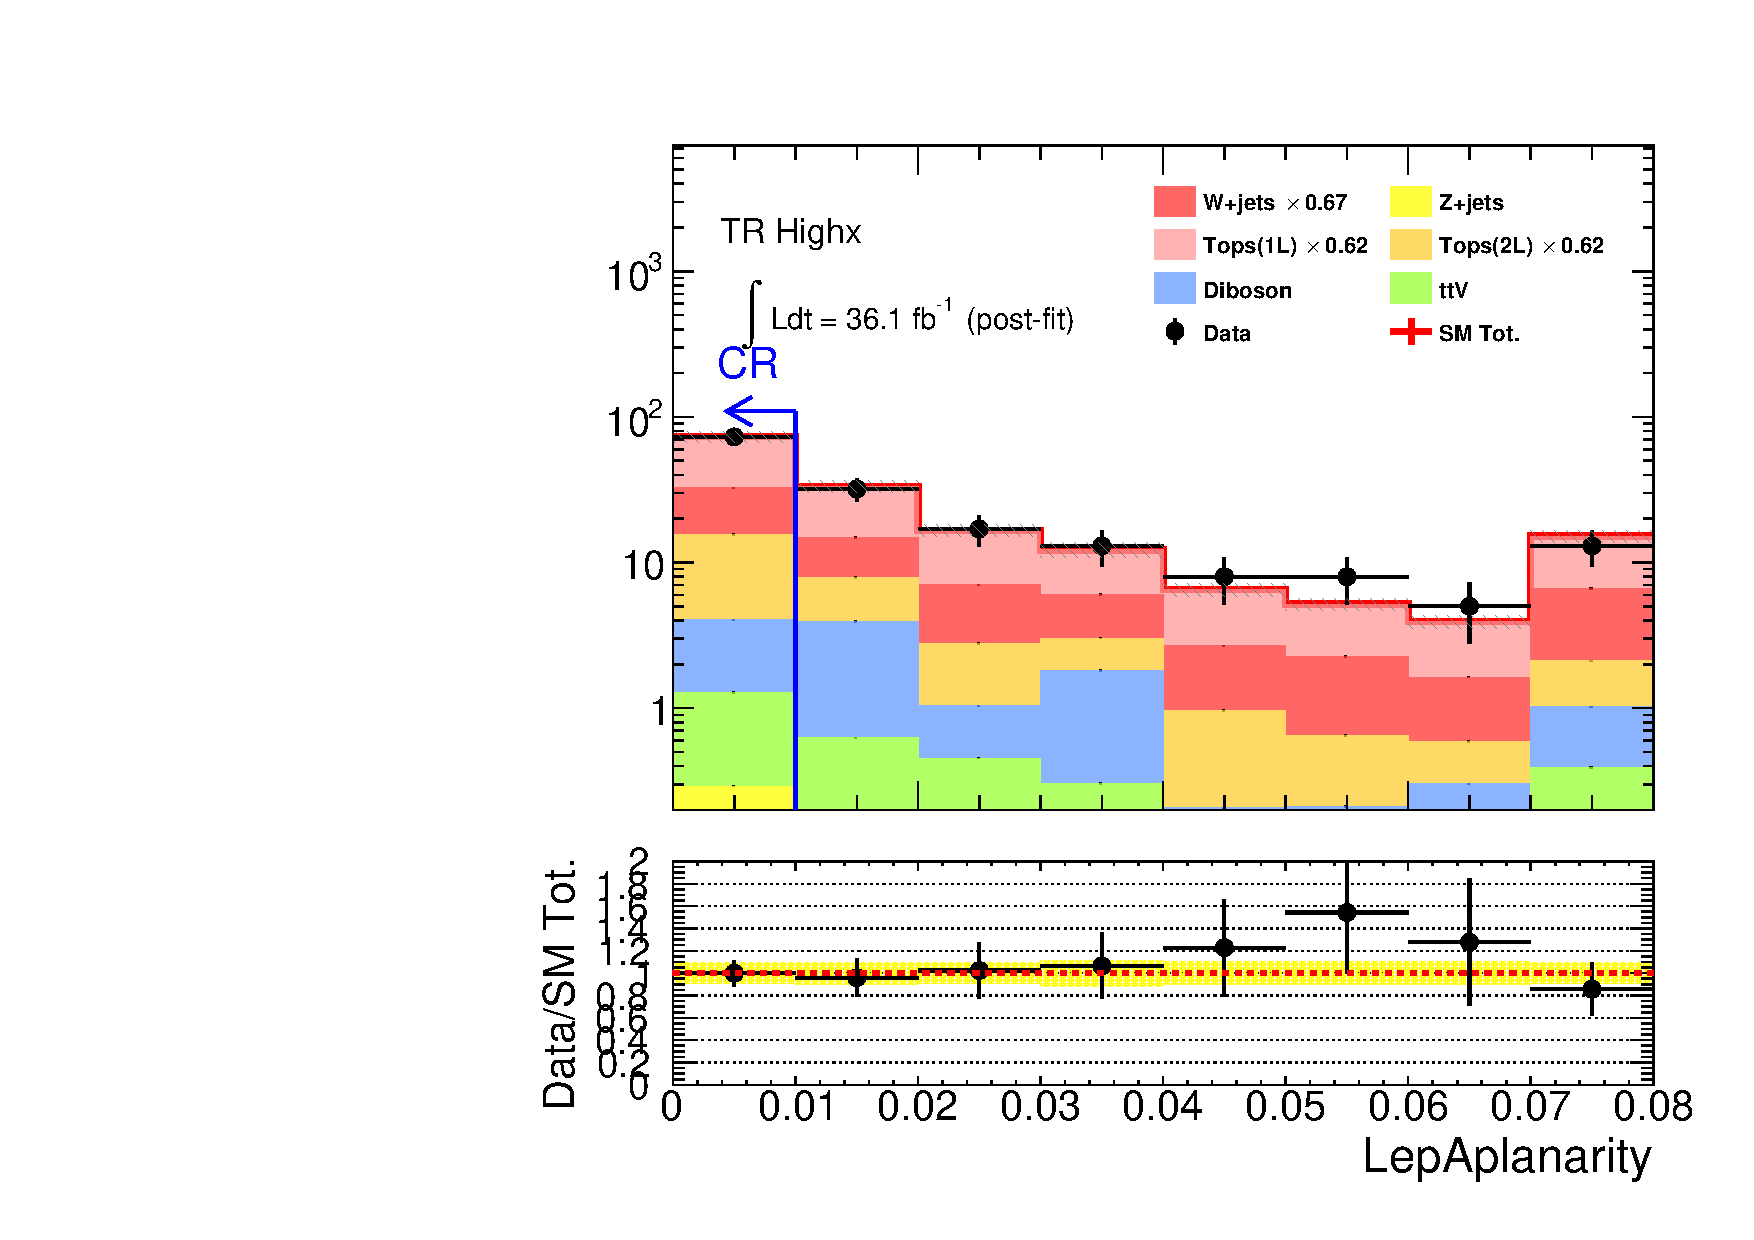
\includegraphics[width=0.41\textwidth]{figures/BGestimation/CRpostFit/TRHighx/LepAplanarity__TRHighx_no_LepAplanarity_postFit_2SFconfig_noYields.pdf}}
   \caption{ 
     Post-fit distruibution of (left) $\mt$ (right) $\apl$.
     (a,b) TR Low-x.
     (c,d) TR High-x.
     The yellow band in the bottom panel represents only statistical error. The overflow is included in the highest bin.  
     \label{fig::BGestimation::CRpostFit::TRVarx}}    
\end{figure}
%----------------------------------


\clearpage
% -------------- 3B ---------
\begin{figure}[h]
  \centering
    \subfigure[]{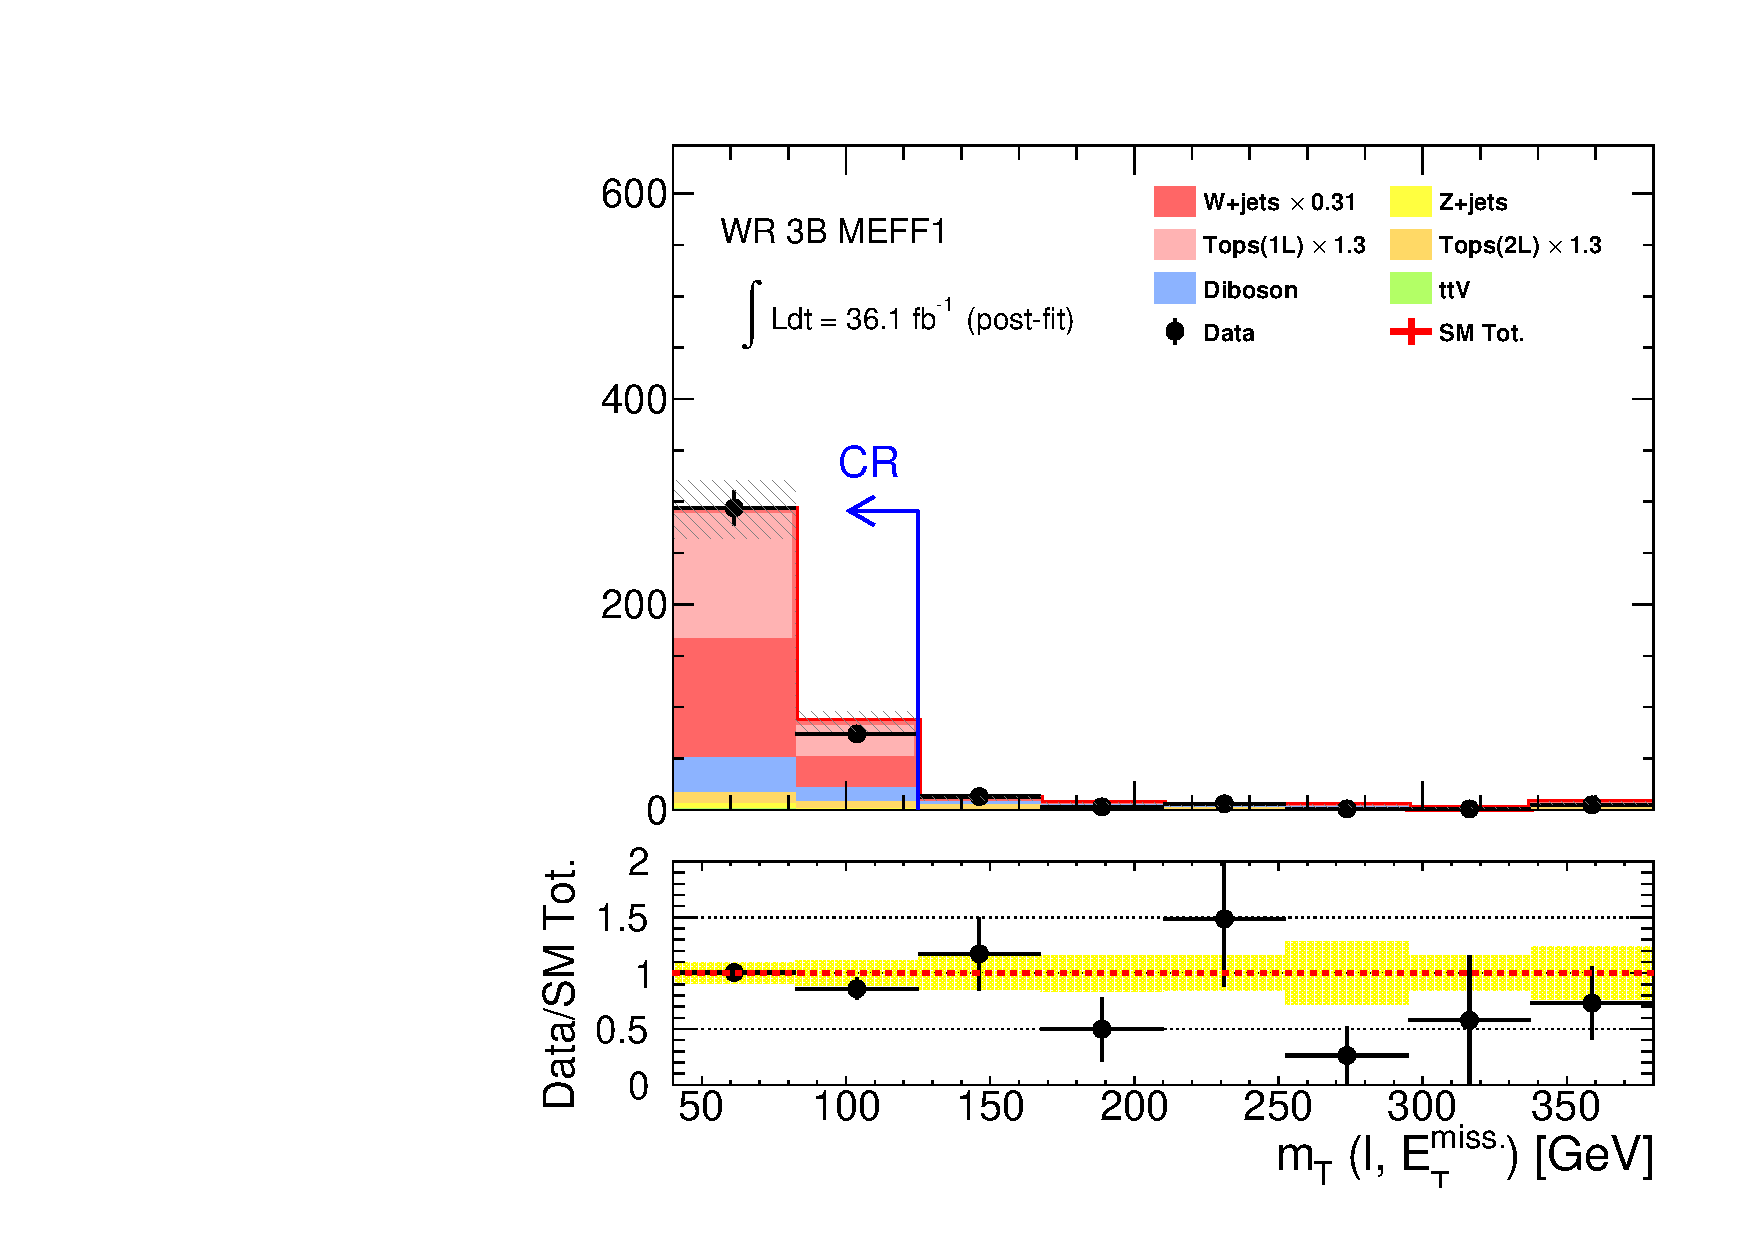
\includegraphics[width=0.41\textwidth]{figures/BGestimation/CRpostFit/WR3BMEFF1/mt__WR3BMEFF1_no_mt_postFit_2SFconfig_noYields.pdf}}
    \subfigure[]{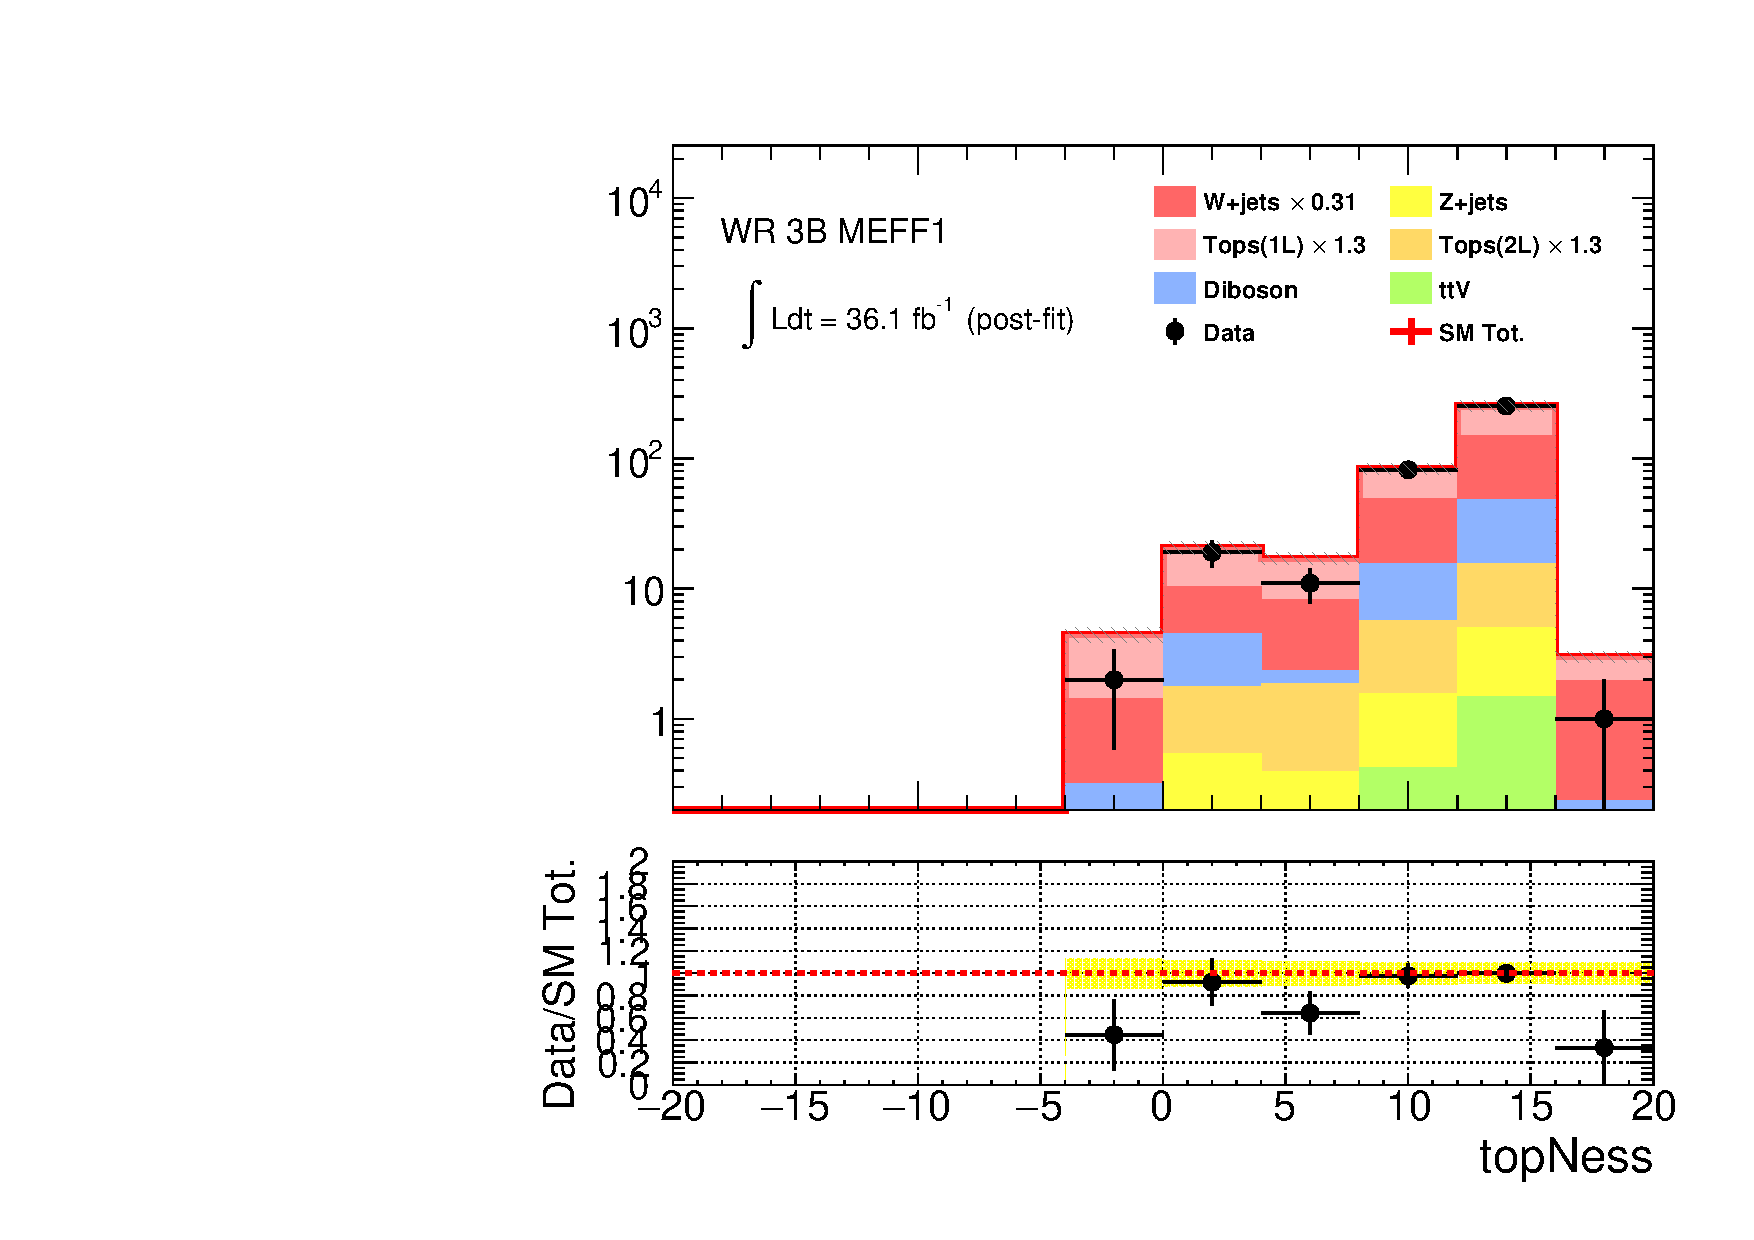
\includegraphics[width=0.41\textwidth]{figures/BGestimation/CRpostFit/WR3BMEFF1/topNess__WR3BMEFF1_postFit_2SFconfig_noYields.pdf}}
    \subfigure[]{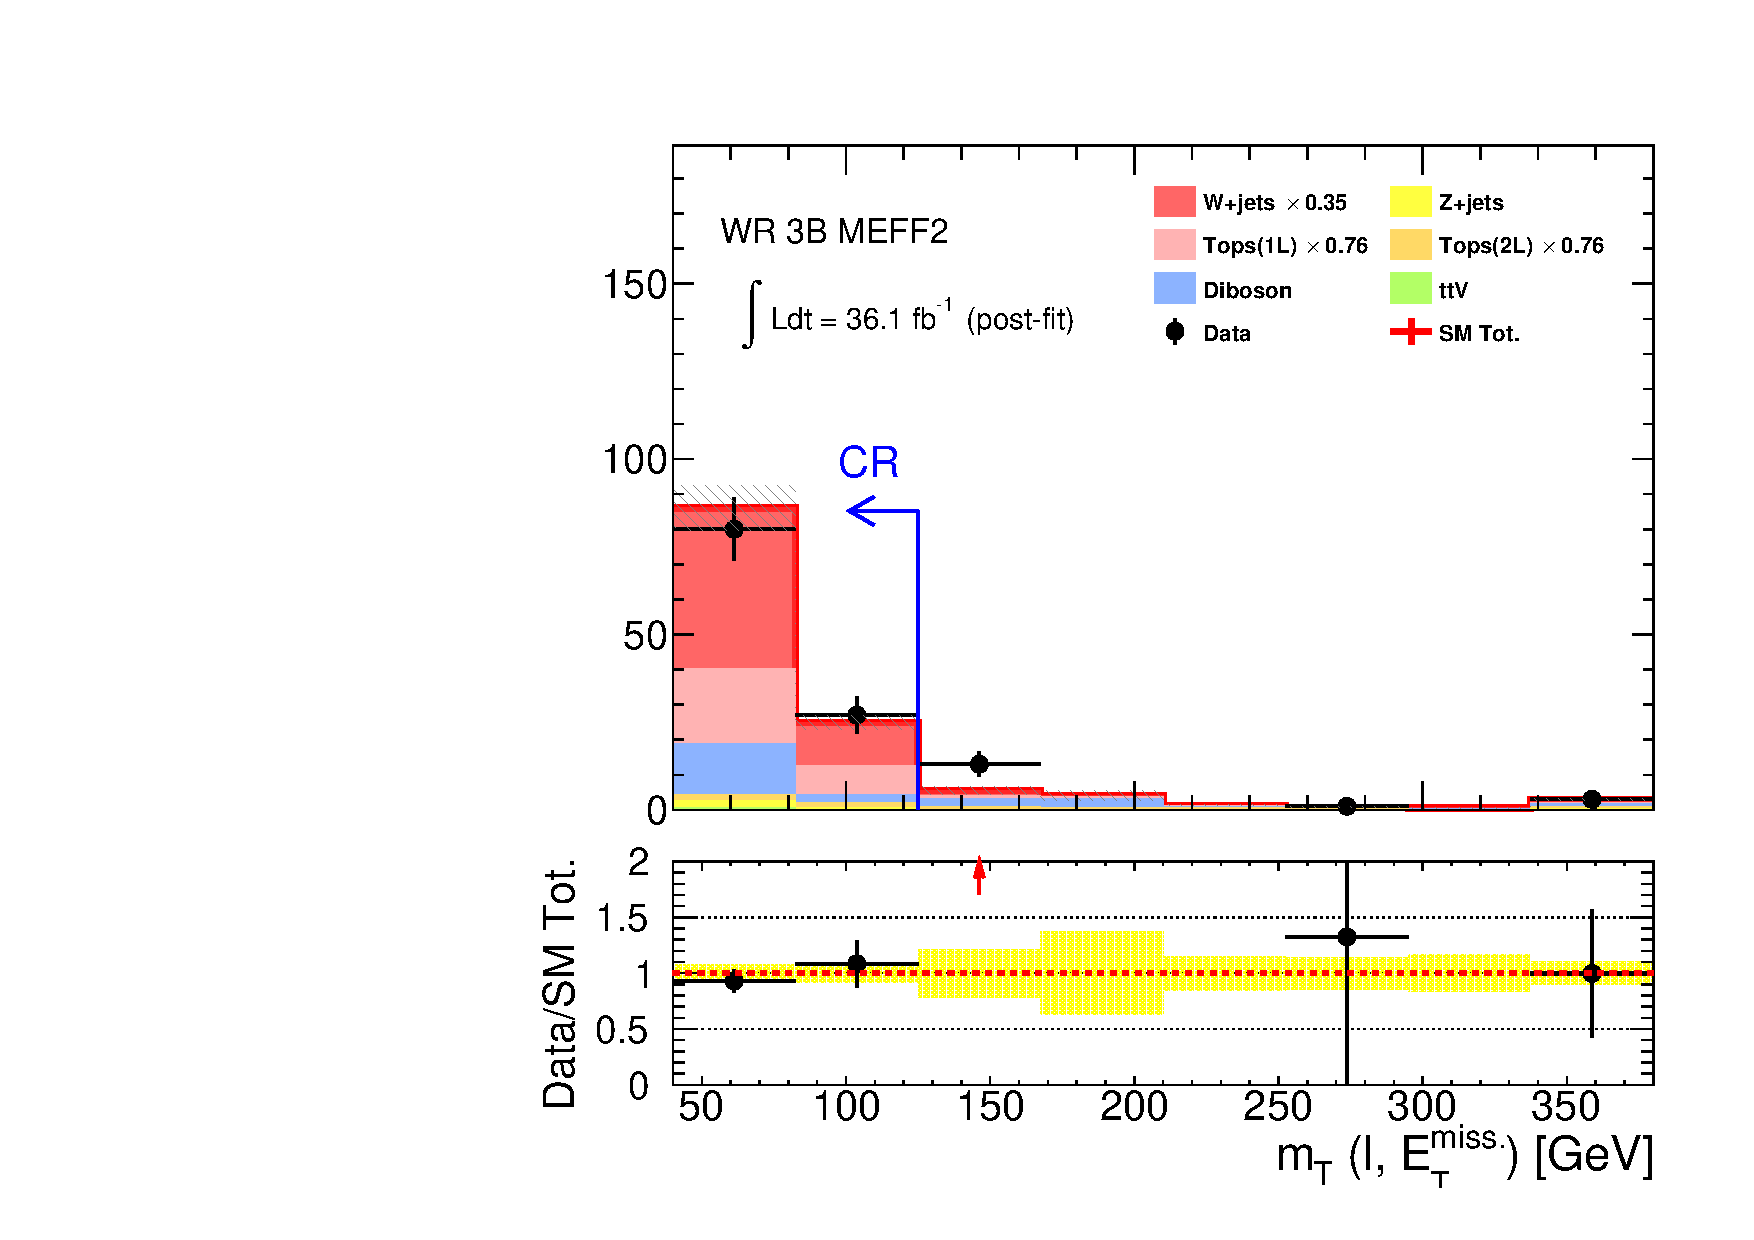
\includegraphics[width=0.41\textwidth]{figures/BGestimation/CRpostFit/WR3BMEFF2/mt__WR3BMEFF2_no_mt_postFit_2SFconfig_noYields.pdf}}
    \subfigure[]{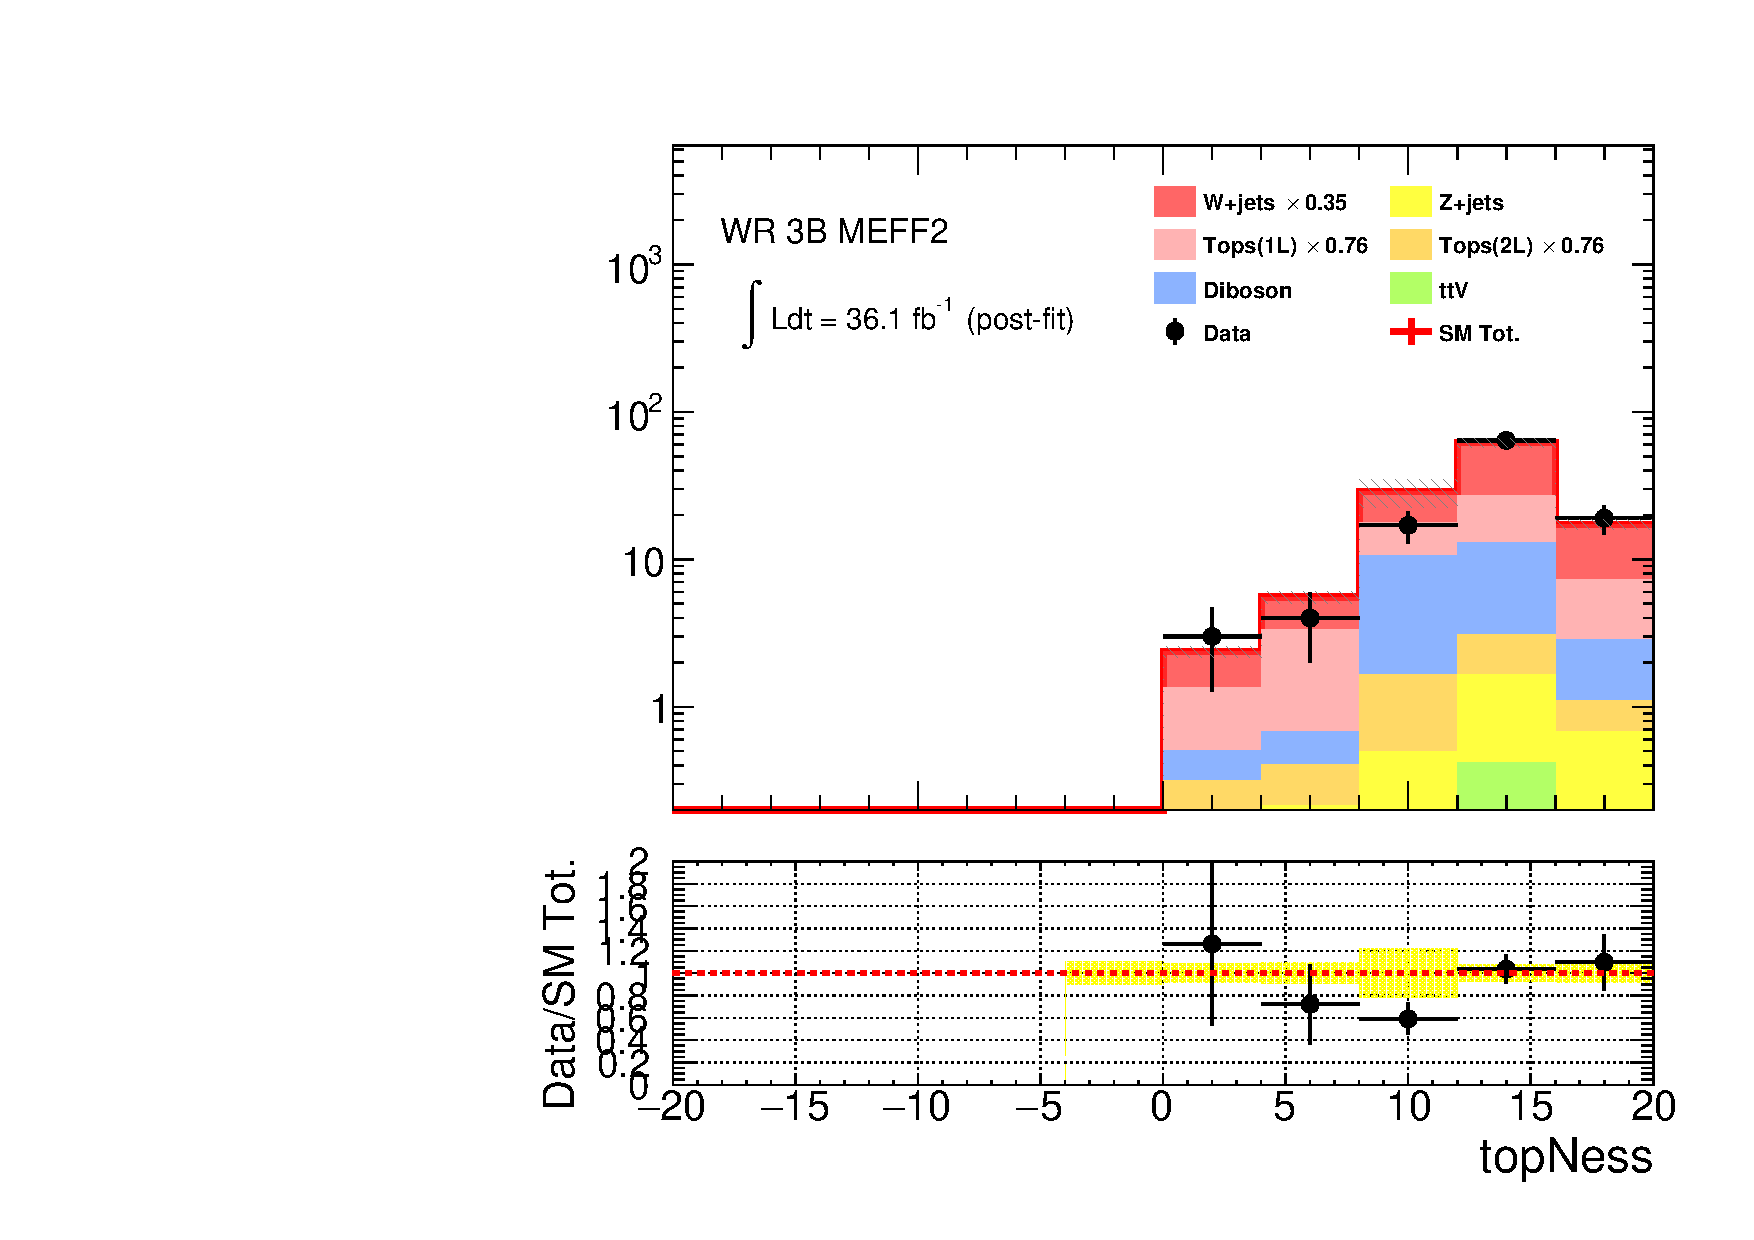
\includegraphics[width=0.41\textwidth]{figures/BGestimation/CRpostFit/WR3BMEFF2/topNess__WR3BMEFF2_postFit_2SFconfig_noYields.pdf}}
   \caption{   
     Post-fit distruibution of (left) $\mt$ (right) topness.
     (a,b) WR 3B-$\meffIncFirst$.
     (c,d) WR 3B-$\meffIncSecond$.
     The yellow band in the bottom panel represents only statistical error. The overflow is included in the highest bin.  
     \label{fig::BGestimation::CRpostFit::WR3B}}    
\end{figure}
%----------------------------------
\begin{figure}[h]
  \centering
    \subfigure[]{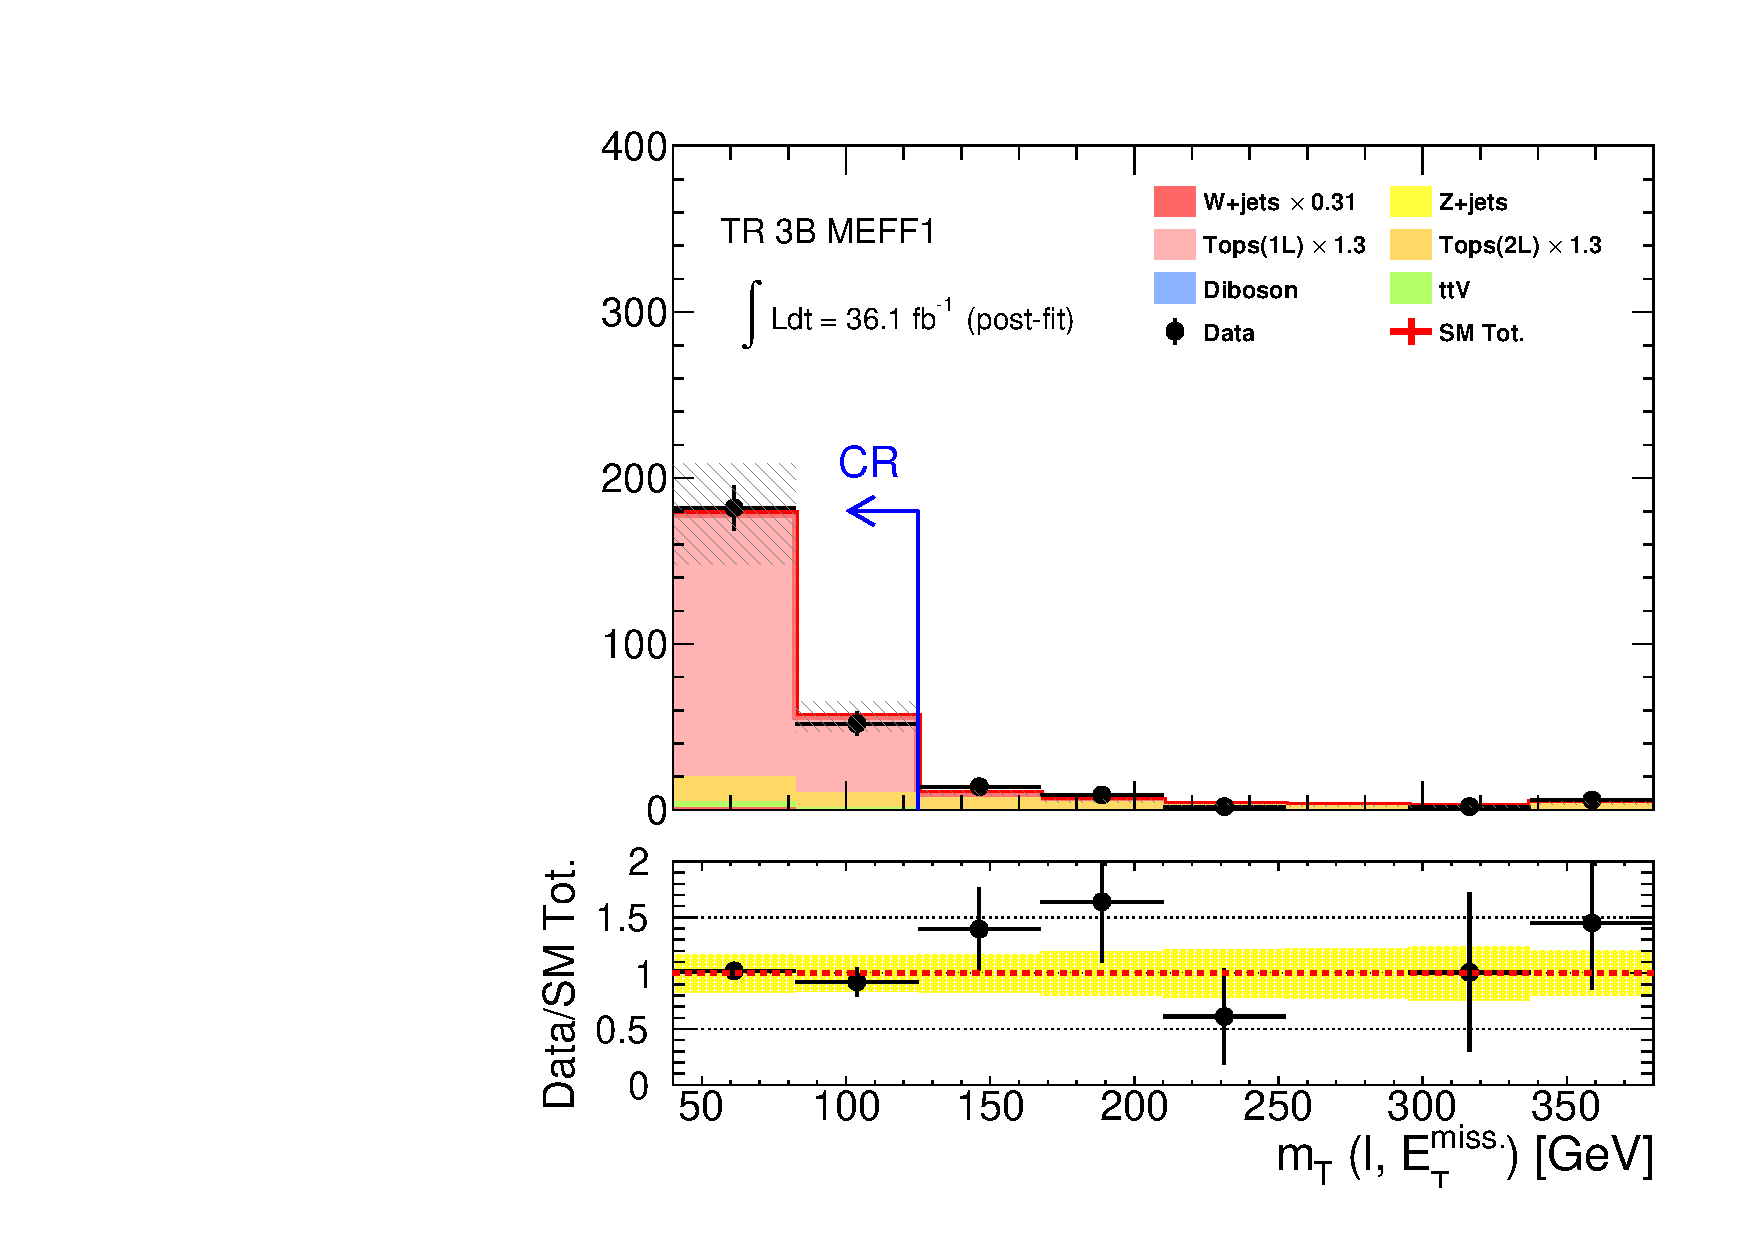
\includegraphics[width=0.41\textwidth]{figures/BGestimation/CRpostFit/TR3BMEFF1/mt__TR3BMEFF1_no_mt_postFit_2SFconfig_noYields.pdf}}
    \subfigure[]{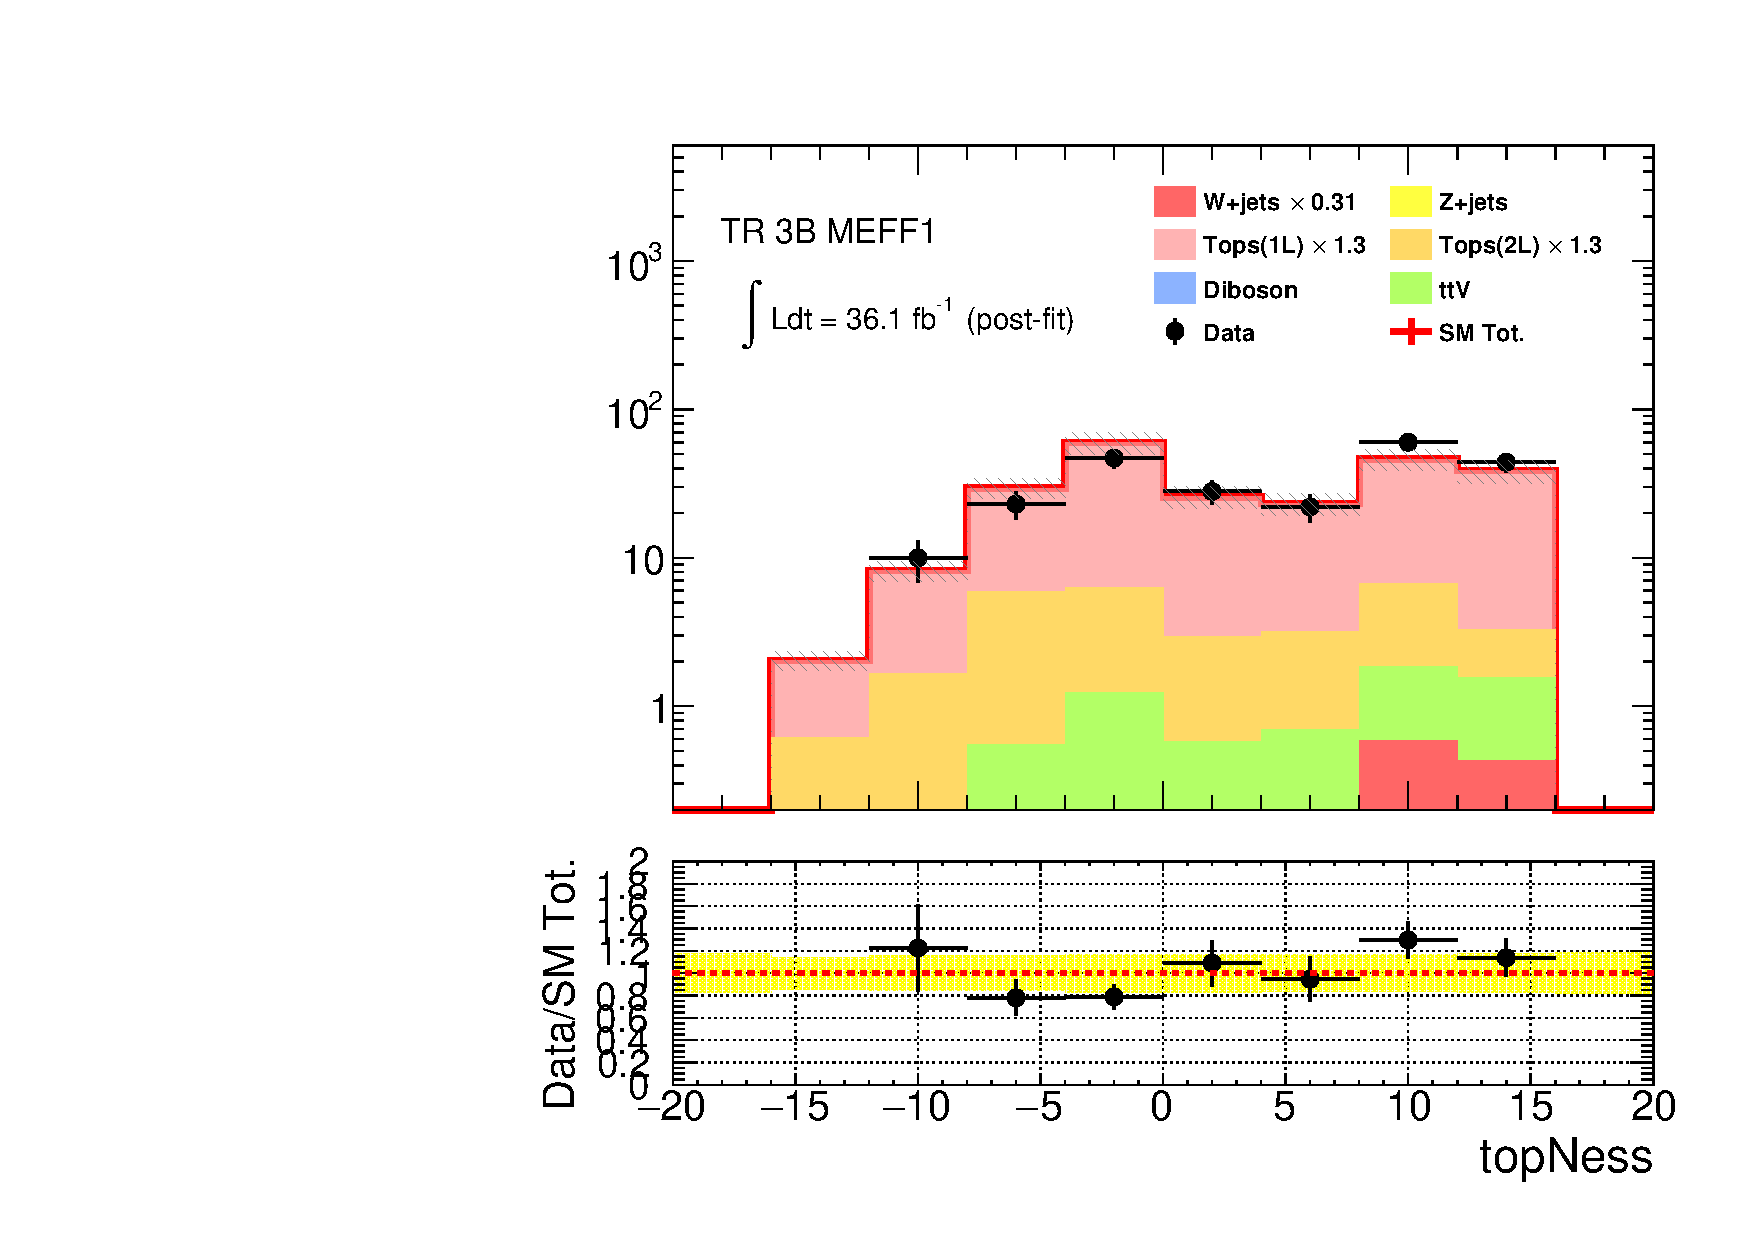
\includegraphics[width=0.41\textwidth]{figures/BGestimation/CRpostFit/TR3BMEFF1/topNess__TR3BMEFF1_postFit_2SFconfig_noYields.pdf}}
    \subfigure[]{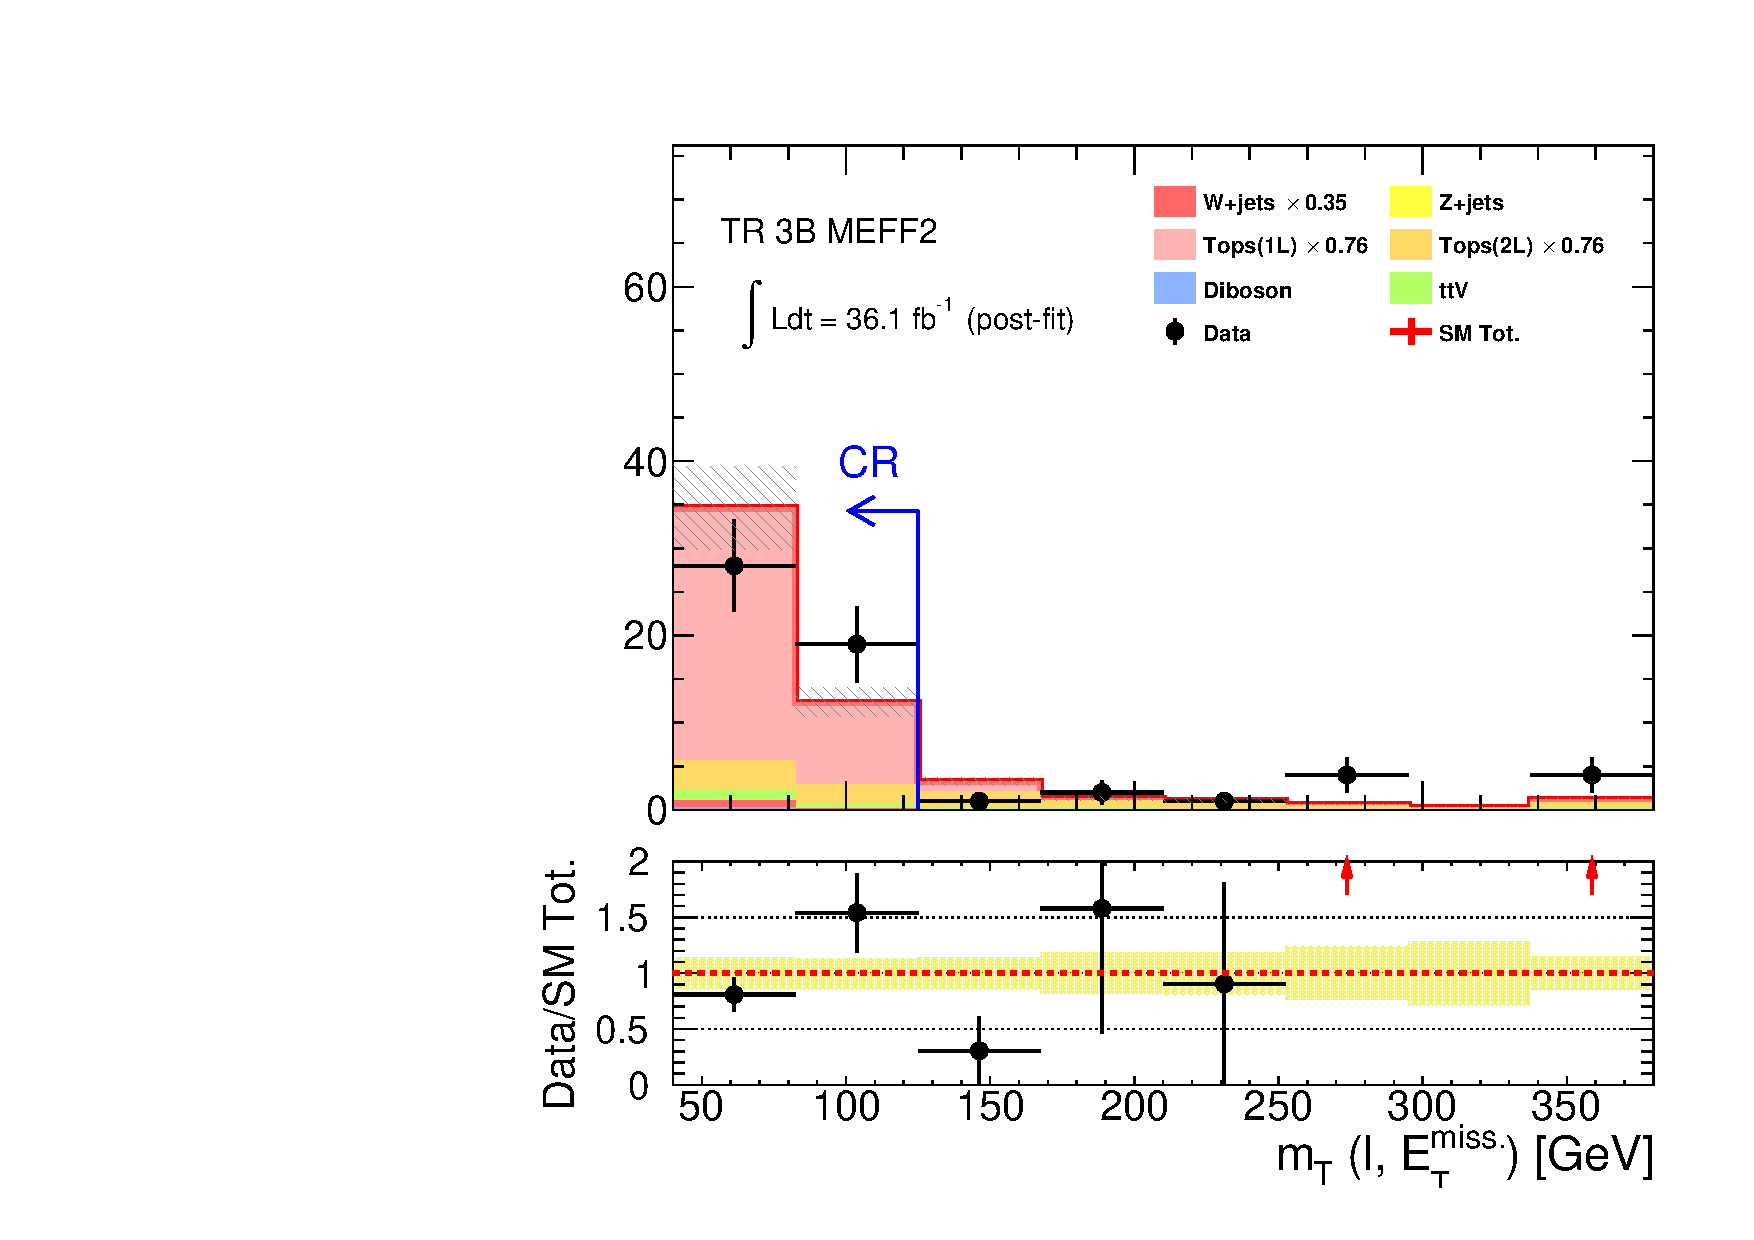
\includegraphics[width=0.41\textwidth]{figures/BGestimation/CRpostFit/TR3BMEFF2/mt__TR3BMEFF2_no_mt_postFit_2SFconfig_noYields.pdf}}
    \subfigure[]{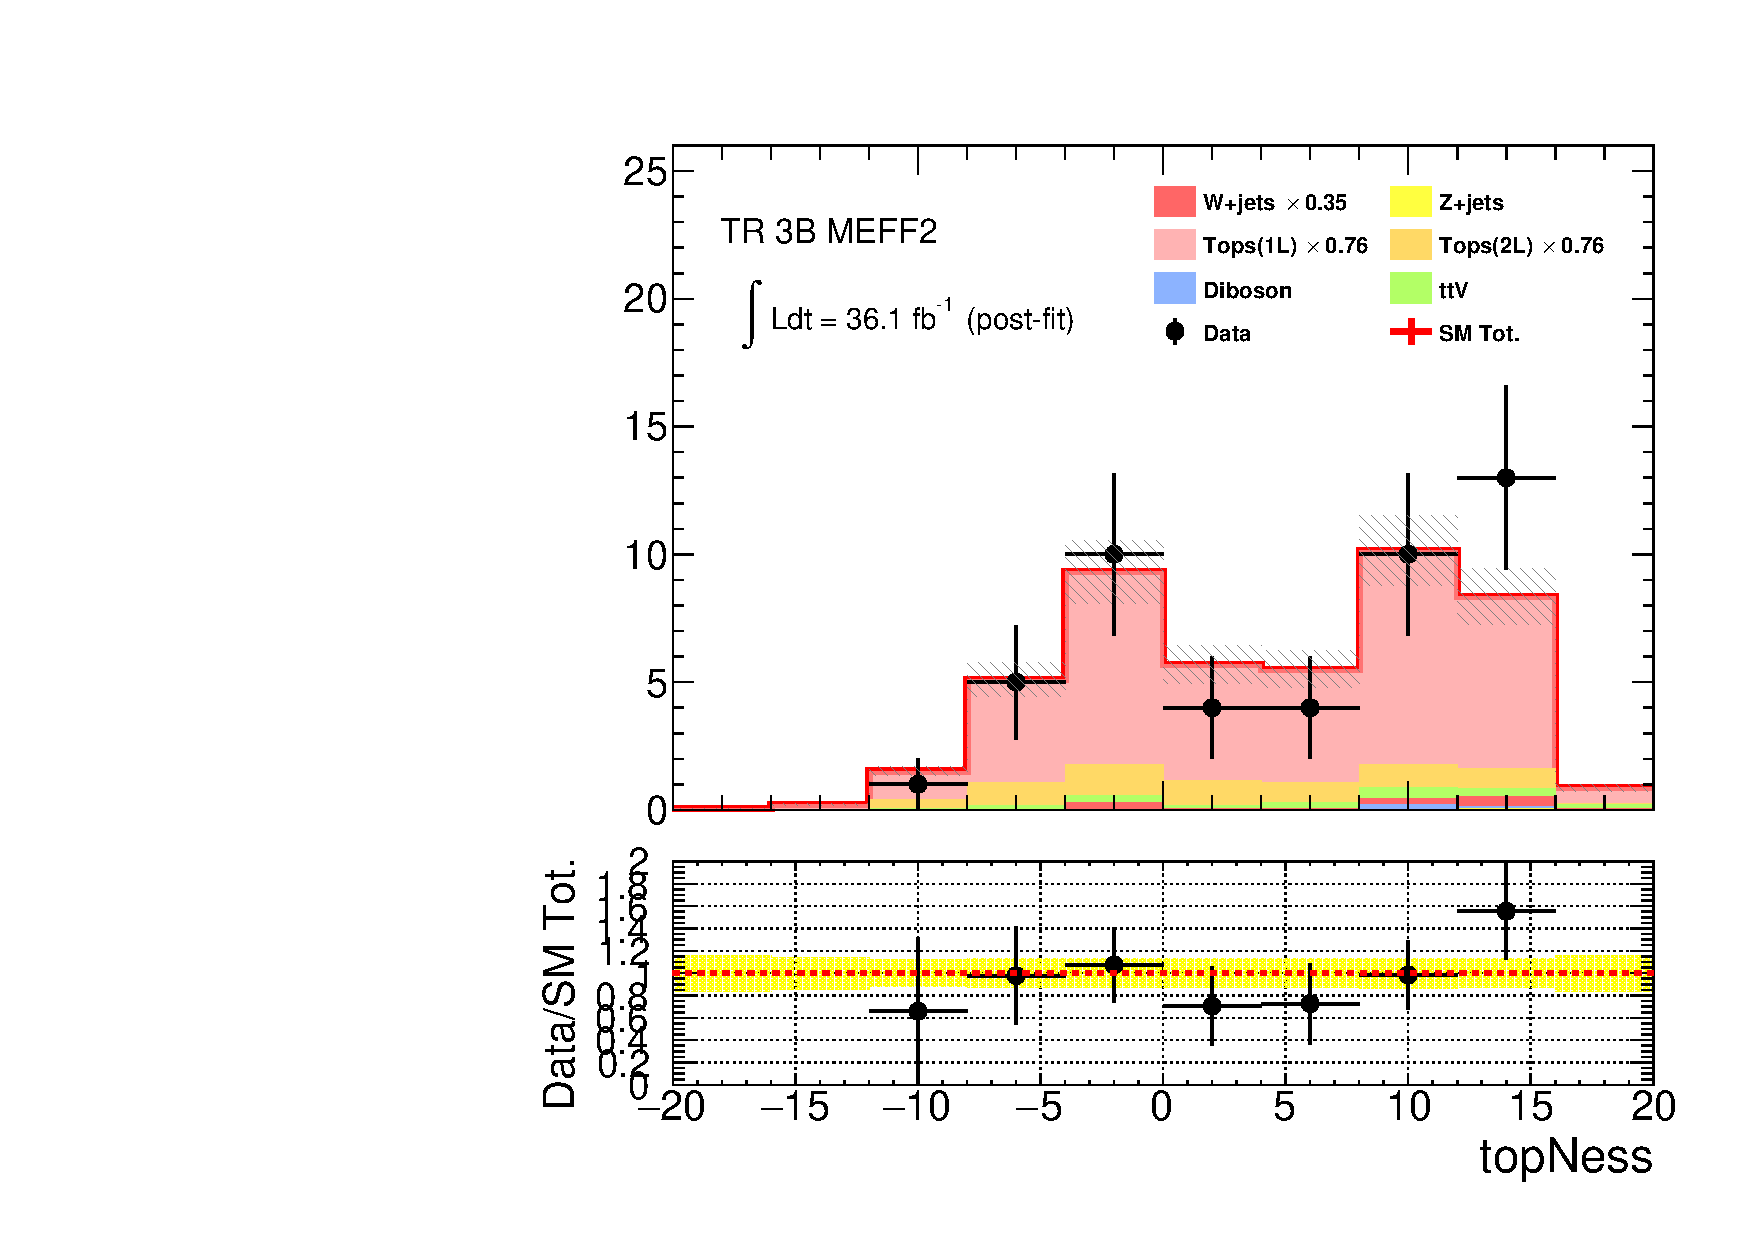
\includegraphics[width=0.41\textwidth]{figures/BGestimation/CRpostFit/TR3BMEFF2/topNess__TR3BMEFF2_postFit_2SFconfig_noYields.pdf}}
   \caption{   
     Post-fit distruibution of (left) $\mt$ (right) topness.
     (a,b) TR 3B-$\meffIncFirst$.
     (c,d) TR 3B-$\meffIncSecond$.
     The yellow band in the bottom panel represents only statistical error. The overflow is included in the highest bin.  
     \label{fig::BGestimation::CRpostFit::TR3B}}    
\end{figure}
%----------------------------------


